\chapter{Measuring the Muon Neutrino Magnetic Moment}\label{sec:NeutrinoMagMoment}

%%% OBJECTIVE / GOAL
In this analysis, I aim to detect a potential signal of the effective muon neutrino magnetic moment in the \gls{NOvA} \gls{ND}. This signal would manifest as an excess of \gls{nuone} elastic scattering interactions at low electron recoil energies, proportional to the value of the effective neutrino magnetic moment, over the \gls{SM} background. If no significant excess is observed, I will establish an upper limit on the effective muon neutrino magnetic moment.

%What are we trying to achieve? We are trying to see the low energy excess of very forward neutrino-on-electron ($\nu$-on-e) events. We can either do this via a counting experiment (possibly with various control samples/regions to control backgrounds and systematics), or with a fit to the energy spectrum of well-selected $\nu$-on-electron events.


%%% WHY - BSM theories, Majorana nature of neutrinos
Detecting the neutrino magnetic moment would provide a definitive evidence of new \gls{BSM} physics, and measuring its value would help identify the appropriate \gls{BSM} theory. As current and planned experiments can only detect an anomalously large neutrino magnetic moment, observing such a signature would strongly suggest that neutrinos are Majorana particles and would have significant implications for astrophysics and cosmology \cite{SnowmassNeutrinoFrontierReport.pdf}.

%"The same types of experimental measurements are also sensitive to more exotic neutrino electromagnetic properties: magnetic moments and millicharges, which would be certainly due to new BSM physics. The discovery of millicharges or anomalously large neutrino magnetic moments would have also important implications for astrophysics and cosmology."\cite{SnowmassNeutrinoFrontierReport.pdf}

%Here just say as a statement of fact that measuring the neutrino magnetic moment would point towards neutrinos being Majorana and would have strong implication for the possibilities of BSM theories. Also that NOvA's highly pure and very intense muon neutrino beam can be used to provide strong limits specifically for the muon neutrino magnetic moments. All these things will be discussed below.

%[Progression review 3] Measuring the neutrino magnetic moment would give us a strong hint towards the new physics \gls{BSM}. If neutrinos are Dirac particles, their magnetic moment would be too small to measure in any current experiments (in most current \gls{BSM} theories). However if neutrinos are Majorana particles, current experiments including \gls{NOvA} and \gls{DUNE} could be able to see its effect. The most sensitive measurement of neutrino magnetic moment is the study of neutrinos elastically scattering off of electrons. If neutrino would have magnetic moment, it would add (without interference) a term to the \gls{nuone} elastic scattering cross section, which is quadratically dependent on the size of the effective magnetic moment and linearly dependent on the inverse of the electron recoil energy. The effective magnetic moment is related to the matrix elements of the dipole magnetic moment via the neutrino oscillation parameters and is different (but interconnected) for different neutrino flavours [3].

%[Thesis readiness review] Neutrinos in theories beyond the Standard Model can obtain a measurable neutrino magnetic moment, which would manifest in the \gls{NOvA} \gls{ND} as an excess of \gls{nuone} elastics scattering interactions in low electron recoil energies. Measuring an enhanced neutrino magnetic moment would point towards the right \gls{BSM} theory, inform us about the necessary energy scale of neutrino mass generation, or point towards neutrinos being Majorana particles. 
%Even though the current global limits on an effective neutrino magnetic moment go beyond the capabilities of the NOvA experiment, these results depend on the detected neutrino flavour and require multiple assumptions when translated to muon neutrinos. 

%[SNOWMASSLOI_NuMMAtNuMuBeams.pdf] Extensions to the Standard Model predict neutrino magnetic moments[1-3], regardless of whether neutrinos are Dirac or Majorana particles. .. Such an unambiguous excess could be interpreted, for example, as evidence[3] for the Majorana nature of the neutrino.


%%% BACKGROUND - history and experiment
%Short history - neutrinos were proposed with magnetic moments, also proposed as a solution to the solar neutrino problem

%[LAMPFAMuNuMM1990.pdf]  Recently, there has been speculation [ 7 ] that this interaction could solve the solar neutrino puzzle, and could explain a possible correlation o f solar neutrino flux with solar (magnetic) activity. If the neutrino magnetic moment were as large as $\mu_\nu\sim\left(10^{-10}-10^{-11}\right)\mu_B$, a significant fraction o f neutrinos would precess in the solar magnetic field from left-handed into sterile right-handed neutrinos and would thereby escape detection on earth.
%[7] is: M.B. Voloshin,M.I. Vysotskiiand L.B. Okun, Yad. Fiz. 44 (1986) 677.

%Current best overall measurements - XENONnT, XENON1T, LZ
The best model-independent experimental results on the neutrino magnetic moment come from experiments searching for dark matter using xenon-based detectors. These highly sensitive detectors detect solar neutrinos, which are part of the background in dark matter searches but can be reanalyzed for other purposes. In 2020, the XENON1T experiment observed \cite{XENON1TExcessNuOnE2020.pdf} a low energy excess of solar neutrinos, which could correspond to a signal from an anomalously large effective magnetic moment within $\mu_{\nu_\odot}\in \left(0.14, 0.29\right)\times 10^{-10} \mu_B$ at $\unit[90]{\%}$ \gls{CL}, where $\nu_\odot$ marks solar neutrinos. However, this result was disfavoured by the follow-up XENONnT experiment in 2022 \cite{XENONnTFirstResults2022.pdf}, which saw no excess and set the current world-leading limit on neutrino magnetic moment at $\mu_{\nu_\odot}<0.063\times 10^{-10}\mu_B$ at $\unit[90]{\%}$ \gls{CL}. Other solar neutrino experiments also reported null results regarding neutrino magnetic moment \cite{LZNuMMResults2022.pdf,BorexinoLimit2017.pdf}, placing less stringent limits on its value. Given some basic assumptions \cite{BorexinoLimit2017.pdf, NuElmagInXENONnTKhan2023.pdf} this limit for solar neutrinos would correspond to a limit on muon neutrino effective magnetic moment of $\mu_{\nu_\mu}<0.137\times 10^{-10}\mu_B$. However, the relationship between effective magnetic moments of different neutrino flavours may be non-trivial, especially in the context of possible new \gls{BSM} physics, and studying muon neutrinos remains an important endeavour \cite{LargeNuMMJointFit2022.pdf}.


%[Progression review 3] The XENON1T experiment published a paper \cite{XENON1TExcessNuOnE2020.pdf} in 2020 showing an excess of neutrino-on-electron events, This was later in 2022 disfavoured by the XENONnT \cite{XENONnTFirstResults2022.pdf} and the LUX-ZEPLIN \cite{LZNuMMResults2022.pdf} experiments, which provided strict constraints of $\mu_{\nu_\odot}<0.64\times 10^{-11}\mu_B$ and $\mu_{\nu_\odot}<1.1\times 10^{-11}\mu_B$ respectively. Given some basic assumptions \cite{BorexinoLimit2017.pdf, NuElmagInXENONnTKhan2023.pdf} this would correspond to more than an order of magnitude stricter limit on muon neutrino effective magnetic moment than NOvA could possibly deliver, but the relationship between effective magnetic moments of different neutrino flavours may be non-trivial (depends on the new physics introduced) and studying muon neutrinos remains an important endeavour \cite{LargeNuMMJointFit2022.pdf}.


%Current best muon mag. moment measurement - LSND

The best results for $\nu_\mu$ and $\overline{\nu}_\mu$ come from accelerator-based stopped pion neutrino sources \cite{LSNDLimits2001.pdf,LAMPFAMuNuMM1990.pdf}, which also do not observe any low energy excess and provide an upper limit on the effective muon neutrino magnetic moment of $\mu_{\nu_\mu}<6.8\times 10^{-10}\mu_B$  at $\unit[90]{\%}$ \gls{CL} \cite{LSNDLimits2001.pdf}. Stopped pion neutrino sources provide a well-understood beams made up of $\nu_\mu$, $\overline{\nu}_\mu$ and $\nu_e$ with energies up to $\unit[52.8]{MeV}$. Slightly looser limits come from pion decay-in-flight accelerator-based measurements (similar to \gls{NOvA})\cite{NuoneForEMProp1990.pdf, Charm2MuonNuMM1995.pdf}, which provide a limit of $\mu_{\nu_\mu}<8.5\times 10^{-10}\mu_B$ at $\unit[90]{\%}$ \gls{CL}.

%[Progression review 3] Best limits \cite{PDG.pdf} for this parameter come from the LSND experiment \cite{LSNDLimits2001.pdf} at $\mu_{\nu_\mu}<6.8\times 10^{-10}\mu_B$.


%%% WHY NOvA IS SPECIAL / USEFUL

Thanks to the very intense and highly pure beam of muon neutrinos and antineutrinos, and a detector designed for the reconstruction and identification of events with electrons in the final state, \gls{NOvA} is well-positioned to provide a highly competitive, and possibly even world-leading, measurement (or limit) of the effective muon neutrino magnetic moment. A previous analysis of \gls{NOvA} \gls{ND} data for a measurement of the effective muon neutrino magnetic moment was presented in a thesis \cite{nuMM-thesis-biaow.pdf}, providing a (statistics-only) limit of $\mu_{\nu_\mu}<15.8\times 10^{-10}\mu_B$ at $\unit[90]{\%}$ \gls{CL}.

%If neutrinos are Dirac particles, their magnetic moment would be too small to be measured in the NOvA near detector. However if neutrinos are Majorana particles, NOvA should be able to measure the neutrino magnetic moment, especially the muon component, by studying scattering of muon neutrino off a free electron. The purity of the NuMI beam would allow NOvA to provide world leading measurement of this component.

%[Progression review 3] The purity of the \gls{NuMI} beam and the use of muon neutrinos and antineutrinos give NOvA a possibility to provide world leading measurement of the muon neutrino effective magnetic moment [8].

%[Thesis readiness review] NOvA benefits from a near pure source of muon neutrinos and antineutrinos and should be able to provide a world leading limit on the muon neutrino magnetic moment.

%[abstract] Measuring an enhanced neutrino magnetic moment would be a clear indication of physics beyond the Standard Model (BSM), shedding light on the correct BSM theory or the potential Majorana nature of neutrinos. It would manifest in the NOvA near detector as an excess of neutrino-on-electron elastic scattering interactions at low electron recoil energies. Leveraging an intense and highly pure muon neutrino beam, along with the finely segmented liquid scintillator detector technology specifically designed for electromagnetic shower separation, enables NOvA to achieve a potentially world-leading sensitivity in probing the effective muon neutrino magnetic moment.

%Old NOvA measurements - Biao
%[Progression review 3]  Biao Wang already made a measurement of neutrino magnetic moment at the NOvA near detector for their thesis \cite{nuMM-thesis-biaow.pdf} and achieved a limit of $\mu_{\nu_\mu}<1.58\times 10^{-9}\mu_B$, however they didn't include a rigorous treatment of systematic uncertainties and their selection could've been considerably more advanced.

%Other NOvA analysis measuring the same signal

Additionally, \gls{nuone} elastic scattering interactions are used in various other analyses in \gls{NOvA}, specifically in efforts to constrain the neutrino beam prediction \cite{NOVA-doc-56383, Nuone_Neutrino2022Poster} and in the search for \gls{LDM} \cite{NOVA-doc-59439}. These analyses developed various tools and methods that can be utilized in the search for neutrino magnetic moment.

%\note{Should I talk about the ND and LDM group's analyses since we're using their tools?}
%The \gls{nuone} interactions are also used in the \gls{ND} group's analysis to constrain the neutrino beam prediction \cite{NOVA-doc-56383}, which relies on the precise theoretical knowledge of the \gls{nuone} interaction cross section. They compare the total number of recorded \gls{nuone} interactions, with background subtracted based on a comparison of data and simulation in a sideband region, to the prediction. Since the number of \gls{nuone} events should only depend on the normalization of the neutrino beam, this analysis should give us a precise validation, or correction, of the neutrino flux normalization. There has been a large amount of work going into this analysis, including making special samples, weights, event classifiers, developing a dedicated event selection, or developing a background subtraction method, among others. To save time and analysis effort, we have taken most of these work at face value and applied it to the neutrino magnetic moment analysis. This will help us get the first good estimate of \gls{NOvA}'s capabilities to constraint (or measure) the neutrino magnetic moment.

%The same detector signature of a single forward going electron shower, as present in the \gls{nuone} events, is also present in the \gls{LDM} analysis \cite{NOVA-doc-59439}. This analysis is using a similar event selection to select the \gls{LDM} events as the \gls{ND} group, only without the final $E\theta^2$ cut (see Sec.\ref{sec:EventSelection}). However, instead of simply comparing the total event counts, the \gls{LDM} analysis is using a CAFAna-based fitting framework to fit for the possible \gls{LDM} signal in a distribution of electron recoil energy multiplied by electron recoil angle squared.

%[Progression review 3] There is a broad group of analysers in the NOvA experiment who study the same neutrino-on-electron events to either provide a constraint on the neutrino beam systematic uncertainty \cite{Nuone_Neutrino2022Poster}, or to study light dark matter. These analysers developed special event resonctruction tools (such as specially trained neural networks), event selections, special enhanced samples, fitting frameworks and systematic uncertinty treatments. All these tools are directly transferable to my analysis and allow me to easily and rapidly provide a baseline version of the neutrino magnetic moment measurement.

%Other significant measurments

%Cosmology

%%% OVERVIEW OF THIS CHAPTER
In this chapter, I will provide an overview of the theory of neutrino electromagnetic interactions in Sec.~\ref{sec:NuMMTheory}, focusing on the effective neutrino magnetic moment and its implications for \gls{nuone} measurements and other theoretical considerations. In Sec.~\ref{sec:NuMMAnalysisOverview}, I will discuss the analysis strategy, the signal and background definition, as well as the data and simulation samples and the analysis weights. Following this, Sec.~\ref{sec:NuMMEventSelection} will explain the selection of events for this analysis, while Sec.~\ref{sec:NuMMResolution} will cover the electron recoil energy and angle resolution studies and the choice of binning. Sec.~\ref{sec:NuMMSystematics} will address the relevant systematic uncertainties and Sec.~\ref{sec:NuMMFitting} will introduce the methods used in the statistical analysis of the measurement. Finally, I will present the results of this analysis in Sec.~\ref{sec:NuMMResults} and discuss their implications in Sec.~\ref{sec:NuMMDiscussion}. Section~\ref{sec:NuMMConclusion} will summarise the findings of this analysis.

\section{Theory of neutrino magnetic moment}\label{sec:NuMMTheory}
\todo{Also check out NeutrinoMassesPheno2007.pdf, sec 6.4}
%Neutrino electromagnetic properties have been proposed since the very beginning by Pauli to solve the discrepancies in the electron beta emission spectra. This was solved by discovering the neutron. Then again, neutrino magnetic moment was proposed as one of the solution to the solar neutrino problem 

% Although in the standard model neutrinos are electrically neutral and do not possess electric or magnetic dipole moments, they have a charge radius which is generated by radiative corrections. [...] In many extensions of the standard model neutrinos also acquire electromagnetic properties through quantum loop effects which allow direct interactions of neutrinos with electromagnetic fields and electromagnetic interactions of neutrinos with charged particles. Hence, the theoretical and experimental study of neutrino electromagnetic interactions is a powerful tool in the search for the fundamental theory beyond the standard model. Moreover, the electromagnetic interactions of neutrinos can generate important effects, especially in astrophysical environments, where neutrinos propagate over long distances in magnetic fields in vacuum and in matter. [nuElmagInt2015.pdf]

% ...the existence of neutrino masses and mixing implies that neutrinos have magnetic moments. Since their values depend on the specific theory which extends the standard model in order to accommodate neutrino masses and mixing, experimentalists and theorists are eagerly looking for them. [nuElmagInt2015.pdf]

%Systematic theoretical studies of neutrino electromagnetic properties started after it was shown that in the extended standard model with right-handed neutrinos the magnetic moment of a massive neutrino is, in general, nonvanishing and that its value is determined by the neutrino mass (Lee and Shrock, 1977; Marciano and Sanda, 1977; Petcov, 1977; Fujikawa and Shrock, 1980; Pal and Wolfenstein, 1982; Shrock, 1982; Bilenky and Petcov, 1987). [nuElmagInt2015.pdf]

%Neutrino electromagnetic properties are important because they are directly connected to fundamentals of particle physics. For example, neutrino electromagnetic properties can be used to distinguish Dirac and Majorana neutrinos, because Dirac neutrinos can have both diagonal and off-diagonal magnetic and electric dipole moments, whereas only the off-diagonal ones are allowed for Majorana neutrinos (Schechter and Valle, 1981; Kayser, 1982, 1984; Nieves, 1982; Pal and Wolfenstein, 1982; Shrock, 1982). This is shown in detail in Secs. III.A and III.B. Another important case in which Dirac and Majorana neutrinos have quite different observable effects is the spin-flavor precession in an external magnetic field discussed in Sec. VI.B. Neutrino electromagnetic properties are also probes of new physics beyond the standard model, because in the standard model neutrinos can have only a charge radius (see Secs. III.C and VII.B). The discovery of other neutrino electromagnetic properties would be a signal of new physics beyond the standard model (Bell et al., 2005, 2006; Bell, 2007; Novales-Sanchez et al., 2008). [nuElmagInt2015.pdf]

As was describe in Sec.~\ref{sec:NeutrinoTheory}, neutrinos in the \gls{SM} are massless and electrically neutral particles. However, even \gls{SM} neutrinos can have electromagnetic interaction through loop diagrams involving charged leptons and the W boson, described by the neutrino charge radius \cite{SnowmassNeutrinoFrontierReport.pdf}.

%But this is only the neutrino charge radius, not the neutrino electric or magnetic moment (maybe also the anapole moment) "Hence, in the standard model the form factor can be interpreted as a neutrino charge radius or as an anapole moment (or as a combination of both). The standard model theory of the neutrino charge radius has a long history, with some controversies which are shortly summarized in the following." [nuElmagInt2015.pdf - sec.VIIB]

%Various theories beyond the Standard Model
In general \gls{BSM} theories, considering interactions with a single photon as shown on Fig.~\ref{fig:FeynmanNuElmagDiagram}, neutrino electromagnetic interactions can be described by an \textit{effective} interaction Hamiltonian \cite{nuElmagInt2015.pdf}
\begin{equation}
\mathcal{H}^{\left(\nu\right)}_{em}\left(x\right)=\sum^N_{k,j=1}\overline{\nu}_k\left(x\right)\Lambda^{kj}_{\mu}\nu_j\left(x\right)A^{\mu}\left(x\right).
\end{equation}
Here $\nu_k\left(x\right), k = 1,...,N,$ are neutrino fields in the mass basis with $N$ neutrino mass states, $\Lambda^{kj}_{\mu}$ is a general vertex function and $A^{\mu}\left(x\right)$ is the electromagnetic field.

\begin{figure}[hbtp]
\centering
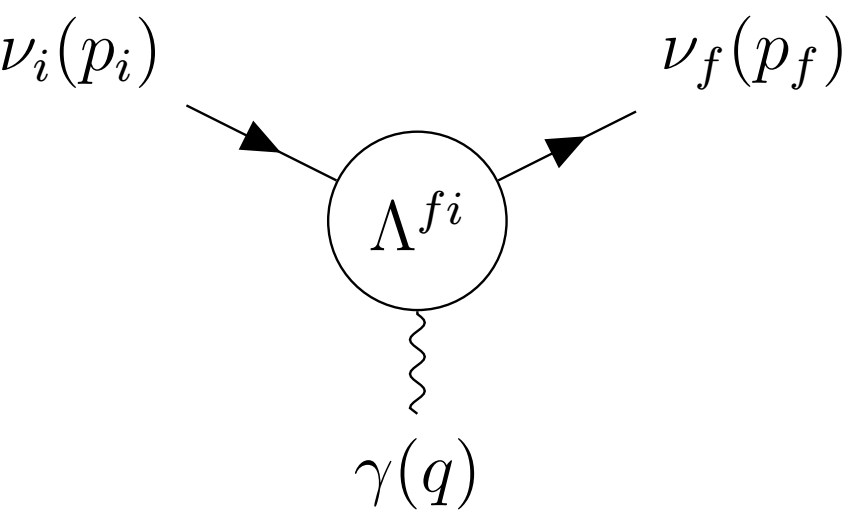
\includegraphics[width=0.4\linewidth]{Plots/NuMM/FeynmanDiagramNuElmagInt.png}
\caption{Effective coupling of neutrinos with one photon electromagnetic field.}
\label{fig:FeynmanNuElmagDiagram}
\end{figure}

\iffalse
The amplitude of neutrino-to-neutrino interaction for \textbf{Dirac} neutrinos is
\begin{equation}
\braket{\nu_f\left(p_f\right)|j^{\left(\nu\right)}_{\mu}\left(x\right)|\nu_i\left(p_i\right)}=
e^{i\left(p_f-p_i\right)x}\overline{u}_f\left(p_f\right)\Lambda^{fi}_{\mu}\left(p_f,p_i\right)u_i\left(p_i\right),
\end{equation}
where $p_f$ and $p_i$ are the final and initial four momentums respectively and $u/\overline{u}$ are the solutions to the Dirac equation for a free particle. We take into account possible transitions between different mass states $\nu_i$ and $\nu_f$ \cite{nuElmagInt2015.pdf}. \todo{also describe what is j}
\fi

The vertex function $\Lambda^{fi}_{\mu}\left(q\right)$ is generally a matrix and in the most general case consistent with the \gls{SM} gauge invariance \cite{MostGeneralNuElmagVectorFunctionExpressionKayser.pdf, MostGeneralNuElmagVectorFunctionExpressionNieves.pdf} can be written in terms of linearly independent products of Dirac matrices $\left(\gamma\right)$ and only depends on the four momentum of the photon $\left(q=p_f-p_i\right)$:
\begin{align}
\Lambda^{fi}_{\mu}\left(q\right)=&
\mathbb{F}^{fi}_1\left(q^2\right)q_{\mu}+
\mathbb{F}^{fi}_2\left(q^2\right)q_{\mu}\gamma_5+
\mathbb{F}^{fi}_3\left(q^2\right)\gamma_{\mu}+
\mathbb{F}^{fi}_4\left(q^2\right)\gamma_{\mu}\gamma_5+\notag\\ &
\mathbb{F}^{fi}_5\left(q^2\right)\sigma_{\mu\nu}q^{\nu}+
\mathbb{F}^{fi}_6\left(q^2\right)\epsilon_{\mu\nu\rho\gamma}q^{\nu}\sigma^{\rho\gamma},
\end{align}
where $\mathbb{F}^{fi}_i\left(q^2\right)$ are six Lorentz invariant form factors and $\delta$ and $\epsilon$ are the Dirac delta and the Levi-Civita symbols respectively.

Applying conditions of hermiticity $\left(\mathcal{H}^{\left(\nu\right)\dagger}_{em}=\mathcal{H}^{\left(\nu\right)}_{em}\right)$ and of the gauge invariance of the electromagnetic field, the vertex function can be rewritten as
\begin{equation}
\Lambda^{fi}_{\mu}\left(q\right)=
\left(\gamma_{\mu}-q_{\mu}\slashed{q}/q^2\right)\left[
\mathbb{F}^{fi}_{Q}\left(q^2\right)+\mathbb{F}^{fi}_{A}\left(q^2\right)q^2\gamma_5\right]-
i\sigma_{\mu\nu}q^{\nu}\left[\mathbb{F}^{fi}_{M}\left(q^2\right)+i\mathbb{F}^{fi}_{E}\left(q^2\right)\gamma_5\right], 
\end{equation}
where $\mathbb{F}^{fi}_Q,\mathbb{F}^{fi}_M,\mathbb{F}^{fi}_E$ and $\mathbb{F}^{fi}_A$ are hermitian matrices representing the charge, dipole magnetic, dipole electric and anapole neutrino form factors respectively. It is clear that the vertex function only depends on the square of the four momentum of the photon $q^2$. In coupling with a real photon $\left(q^2=0\right)$ these form factors become the neutrino charge and magnetic, electric and anapole moments respectively. Additionally, the neutrino charge radius corresponds to the second term in the expansion of the charge form factor \cite{nuElmagInt2015.pdf}.

The above expression can be simplified \cite{NeutrinoPropertiesSnowmass2022.pdf} as
\begin{equation}
\Lambda^{fi}_{\mu}\left(q\right)=\gamma_{\mu}\left(Q_{\nu_{fi}}+\frac{q^2}{6}\langle r^2\rangle_{\nu_{fi}}\right)-i\sigma_{\mu\nu}q^{\nu}\mu_{\nu_{fi}},
\end{equation}
where $Q_{\nu_{fi}}$, $\langle r^2\rangle_{\nu_{fi}}$, and $\mu_{\nu_{fi}}$ are the neutrino charge, effective charge radius (also containing anapole moment), and an effective magnetic moment (also containing electric moment) respectively. This is possible thanks to the similar effects of the neutrino charge radius and the anapole moment, or of the neutrino magnetic and electric moments, on neutrino interactions. Therefore, these are the three neutrino electromagnetic properties (charge, effective charge radius and effective magnetic moment) measured in the experiments.

The neutrino electric charge is primarily constrained through measurements of the neutrality of matter and cosmological observations, which provide much better constraints than neutrino oscillation experiments \cite{nuElmagInt2015.pdf}. On the other hand, the neutrino charge radius would manifest as an increase in the size of the \gls{nuone} elastic scattering coupling constants, allowing it to be studied in neutrino oscillation experiments such as \gls{NOvA}. Additionally, the value of the neutrino charge radius in the \gls{SM} is only an order of magnitude smaller than the current world-leading limits \cite{PDG.pdf} and measuring it could either confirm the validity neutrino interactions in the \gls{SM}, or open possibilities to non-standard contributions to neutrino scattering \cite{nuElmagInt2015.pdf}. However, measurement of the neutrino charge radius is not part of this analysis, but may be included in the future re-analysis of the \gls{NOvA} \gls{ND} data.

%Neutrino electric charge is heavily constraint by the measurements on the neutrality of matter (since generally neutrinos having an electric charge would also mean that neutrons have charge which would affect all heavier nuclei). It is also constrained by the SN1987A, since neutrino having an effective charge would lengthen its path through the extragalactic magnetic fields and would arrive on earth later. It can also be obtained from nu-on-e scatter from the relationship between neutrino millicharge and magnetic moment. [nuElmagInt2015.pdf - sec. VIIA]

%The neutrino charge radius is determined by the second term in the expansion of the neutrino charge form factor and can be interpreted using the Fourier transform of a spherically symmetric charge distribution. It can also be negative since the charge density is not a positively defined quantity. In the SM the charge radius has the form of (possible other definitions exist)
%\begin{equation}
%\langle r_{\nu_l}^2\rangle_{\textsf{SM}}=\frac{G_{\textsf{F}}}{4\sqrt{2}\pi^2}\left[3-2\log\left(\frac{m_l^2}{m_W^2}\right)\right].
%\end{equation}
%This corresponds to $\langle r_{\nu_{\mu}}^2\rangle_{\textsf{SM}}=2.4\times 10^{-33}\ \unit{cm^2}$ and similar scale for other neutrino flavours. [nuElmagInt2015.pdf - sec. VIIB]

%[nuElmagInt2015.pdf - sec. VIIB]
%The effect of the neutrino charge radius on the neutrino-on-electron scattering cross section is through the following shift of the vector coupling constant (Grau and Grifols, 1986; Degrassi, Sirlin, and VMarciano, 1989; Vogel and Engel, 1989; Hagiwara et al., 1994):
%\begin{equation}
%g_V^{\nu_l}\rightarrow g_V^{\nu_l}+\frac{2}{3}m_W^2\langle r_{\nu_l}^2\rangle\sin^2\theta_W
%\end{equation}

%[nuElmagInt2015.pdf - sec. VIIB]
%The current experimental limits for muon neutrinos are from \todo{check the current exp. limits}  Hirsch, Nardi, and Restrepo (2003) who obtained the following 90\% C.L. bounds on $\langle r_{\nu_\mu}^2\rangle$ from a reanalysis of CHARM-II (Vilain et al., 1995) and CCFR (McFarland et al.,1998) data:
%\begin{equation}
%-0.52\times 10^{-32}<\langle r_{\nu_\mu}^2\rangle<0.68\times 10^{-32}\ \unit{cm^2}
%\end{equation}

%"In the standard model, neutrinos have small charge radii induced by radiative corrections. The predicted values of the electron and muon neutrino charge radii are less than an order of magnitude smaller than the current experimental upper limits and can be tested in the next generation of accelerator and reactor experiments through the observation of neutrino-electron elastic scattering and CEvNS. Precision measurements of the neutrino charge radii would either be an important confirmation of the standard model, or would discover new physics. The same types of experimental measurements are also sensitive to more exotic neutrino electromagnetic properties: magnetic moments and millicharges, which would be certainly due to new BSM physics. The discovery of millicharges or anomalously large neutrino magnetic moments would have also important implications for astrophysics and cosmology."\cite{SnowmassNeutrinoFrontierReport.pdf}

\iffalse
For antineutrinos the form factors are transformed as:
\begin{equation}\label{eqAnu1}
\overline{\mathbb{F}}^{fi}_{\Omega}=-\mathbb{F}^{if}_{\Omega}=-\left(\mathbb{F}^{fi}_{\Omega}\right)^{\star} \ \ \ \Omega=Q,M,E,
\end{equation}
\begin{equation}\label{eqAnu2}
\overline{\mathbb{F}}^{fi}_{A}=\mathbb{F}^{if}_{A}=\left(\mathbb{F}^{fi}_{A}\right)^{\star}.
\end{equation}
\todo{maybe describe what does this mean?}

In case of \textbf{Majorana neutrinos}, the general expression for the vertex function in terms of charge, magnetic, electric and anapole form factors looks the same as for Dirac neutrinos.
\todo{so does that mean that the interaction amplitude can be written in the same way for both Dirac and Majorana neutrinos?} However, since Majorana antineutrinos are the same particle as Majorana neutrinos, from eq.\ref{eqAnu1},\ref{eqAnu2} we can see that:
\begin{equation}\label{eqAntisymmetryCondition}
\mathbb{F}^M_{\Omega}=-\left(\mathbb{F}^M_{\Omega}\right)^T \ \ \ \Omega=Q,M,E,
\end{equation}
\begin{equation}
\mathbb{F}^M_{A}=\left(\mathbb{F}^M_A\right)^T.
\end{equation}
Therefore the Majorana charge, magnetic and electric form factor matrices are antisymmetric and the anapole form factor matrix is symmetric. This means that Majorana neutrino doesn't have any diagonal charge and dipole magnetic and electric moments, but it can have transition  charge and magnetic and electric moment \cite{nuElmagInt2015.pdf}.
\todo{Explain why is this worth mentioning or remove it if it's not}
\fi

%%%%%%%%%%%%%%%%%%%%%%%%%%%%%%%%%%%%%%%%
\subsection{Neutrino electric and magnetic dipole moments}
The size and effect of neutrino electromagnetic properties depend on the specific \gls{BSM} theory applied. Evaluating one loop diagrams in the minimally extended \gls{SM} with three right-handed Dirac neutrinos, as described in Sec.~\ref{sec:NuMass}, gives the first approximation of the electric and magnetic moments, which are $3\times 3$ matrices, with elements:
\begin{equation}\label{eq:DiracMagMomExpression}
\begin{rcases}
\mu^D_{kj}\\
i\epsilon^D_{kj}
\end{rcases}
\simeq\frac{3eG_F}{16\sqrt{2}\pi^2}\left(m_k\pm m_j\right)\left(\delta_{kj}-\frac{1}{2}\sum_{l=e,\mu ,\tau}U^{\star}_{lk}U_{lj}\frac{m_l^2}{m_W^2}\right),
\end{equation}
where $m_k,m_j$ are the neutrino masses and $m_l$ are the masses of charged leptons which appear in the loop diagrams \cite{nuElmagInt2015.pdf}. The $D$ superscript denotes Dirac neutrinos and $M$ Majorana neutrinos throughout the section. Also, $e$ is the electron charge, $G_F$ is the Fermi coupling constant, and $U$ is the \gls{PMNS} neutrino oscillation matrix. Higher order electromagnetic corrections were neglected, but can also have a significant contribution, depending on the theory.

It can be seen that Dirac neutrinos have no diagonal electric moments $\left(\epsilon_{kk}^D=0\right)$ and their diagonal magnetic moments are approximately
\begin{equation}\label{eq:DiagMagMomVal}
\mu_{kk}^D\simeq\frac{3eG_Fm_k}{8\sqrt{2}\pi^2}\simeq 3.2\times 10^{-19}\left(\frac{m_k}{\textsf{eV}}\right)\mu_B,
\end{equation}
where $\mu_B$ is the Bohr magneton which represents the value of the electron magnetic moment \cite{nuElmagInt2015.pdf}. Neutrino magnetic moments are therefore strongly suppressed by the smallness of neutrino masses, with theoretical predictions in Eq.~\ref{eq:DiagMagMomVal} several orders of magnitude below the reach of current experiments \cite{NeutrinoPropertiesSnowmass2022.pdf}.

The transition magnetic moments from Eq.~\ref{eq:DiracMagMomExpression} are suppressed with respect to the largest of the diagonal magnetic moments by at least a factor of $10^{-4}$ due to the $m_W^2$ in the denominator. The transition electric moments are even smaller due to the mass difference in Eq.~\ref{eq:DiracMagMomExpression}. Therefore an experimental observation of a magnetic moment larger than in Eq.~\ref{eq:DiagMagMomVal} would indicate physics beyond the minimally extended \gls{SM} \cite{nuElmagInt2015.pdf,nuMMMajoranaBounds2006.pdf}.

\cite{NeutrinoMassesPheno2007.pdf} In general models, however, there is no such direct proportionality between the neutrino mass and its coupling to the electromagnetic interactions. Consequently neutrinos can have sizeable magnetic moment and/or electric dipole moment (EDM) couplings which can show a non-trivial flavor structure. Thus the existence of any electromagnetic neutrino moment well above the expectation in Eq. (269) would signal that some special mechanism, which goes beyond the SM, is at work. Therefore, neutrino electromagnetic properties are interesting probes of new physics.

\cite{NeutrinoMassesPheno2007.pdf} There is also another important difference between Majorana and Dirac neutrinos for the spin-flavor precession mechanism. For Dirac Neutrinos, the resulting states are right-handed neutrinos which are sterile and therefore undetectable while for Majorana neutrinos spin-flavor precession converts left-handed $\nu_e$ into right-handed $\overline{\nu}_\mu$ or $\overline{\nu}_\tau$, which can be detected in accordance with the SNO NC measurement.

\cite{NeutrinoMassesPheno2007.pdf} ...it is important to notice that the square of the effective MM is independent of the basis chosen (mass/flavour) [255] and it only depends on the neutrino flavour at the source and on its propagation.

[PDG] For Majorana neutrinos the matrix $\lambda$ is antisymmetric and only transition moments are allowed, while for Dirac neutrinos $\lambda$ is a general $3\times 3$ matrix.

\todo{Actually write why these values are different for Majorana neutrinos than for Dirac neutrinos}
Majorana neutrinos in a minimal extension can be obtained by either adding a $\textsf{SU}\left(2\right)_L$ Higgs triplet, or right handed neutrinos together with a $\textsf{SU}\left(2\right)_L$ Higgs singlet \cite{nuElmagInt2015.pdf}. If we neglect the Feynman diagrams which depend on the model of the scalar sector, the magnetic and electric dipole moments are
\begin{equation}
\mu_{kj}^M\simeq -\frac{3ieG_F}{16\sqrt{2}\pi^2}\left(m_k+m_j\right)\sum_{l=e,\mu ,\tau}\operatorname{Im}\left[U^{\star}_{lk}U_{lj}\right]\frac{m_l^2}{m_W^2},
\end{equation}
\begin{equation}
\epsilon_{kj}^M\simeq \frac{3ieG_F}{16\sqrt{2}\pi^2}\left(m_k-m_j\right)\sum_{l=e,\mu ,\tau}\operatorname{Re}\left[U^{\star}_{lk}U_{lj}\right]\frac{m_l^2}{m_W^2}.
\end{equation}
These are difficult to compare to the Dirac case, due to possible presence of Majorana phases in the \gls{PMNS} matrices, but it is clear that they have the same order of magnitude as Dirac transition dipole moments. However, the neglected model dependent contributions can enhance the transition dipole moments \cite{nuElmagInt2015.pdf}.

[PDG]  In the standard electroweak theory extended to include neutrino masses (see FUJIKAWA 80) $\mu_\nu=3eG_Fm_\nu/\left(8\pi^2\sqrt{2}\right)=3.2\times10^{-19}\frac{m_\nu}{\unit{eV}}\mu_B$, i.e. it is unobservably small given the known small neutrino masses. In more general models there is no longer a proportionality between neutrino mass and its magnetic moment, even though only massive neutrinos have nonvanishing magnetic moments without fine tuning.

\todo{Re-read the natural upper bounds paper}
It is possible \cite{nuMMMajoranaBounds2006.pdf} to obtain a `natural' upper limits on the size of the neutrino magnetic moment by calculating its contribution to the neutrino mass by standard model radiative corrections. \todo{I don't think this is clear enough, how is this done} For Dirac neutrinos, the radiative correction induced by neutrino magnetic moment, generated at an energy scale $\Lambda_{NP}$, to the neutrino mass is generically
\begin{equation}
m_{\nu}^D\sim\frac{\mu_{\nu}^D}{3\times 10^{-15}\mu_B}\left[\Lambda\left(\textsf{TeV}\right)\right]^2\textsf{eV}.
\end{equation}
So for $\Lambda_{NP}\simeq 1\textsf{TeV}$ and $m_{\nu}\lesssim 0.3\textsf{eV}$ the limit becomes $\mu_{\nu}^D\lesssim 10^{-15}\mu_B$. This applies only if \gls{NP} is well above the electroweak scale ($\Lambda_{EW} \sim 100\textsf{GeV}$) \todo{Finish this sentence}. However, there are theories that contain a Dirac neutrino magnetic moment higher than this limit, for example in frameworks of minimal super-symmetric standard model, by adding more Higgs doublets, or by considering large extra dimensions \todo{Add references to the specific theories?} \cite{nuElmagInt2015.pdf}.

Similar limit for Majorana neutrino magnetic moment would be less stringent than for Dirac neutrinos due to the antisymmetry of the Majorana neutrino magnetic moment form factors \todo{Probably explain here a bit more what does this mean}. Considering $m_{\nu}\lesssim 0.3\textsf{eV}$, the limit can be expressed as 
\begin{align}
\mu_{\tau\mu},\mu_{\tau e} &\lesssim 10^{-9}\left[\Lambda\left(\textsf{TeV}\right)\right]^{-2}\\
\mu_{\mu e} &\lesssim 3\times 10^{-7}\left[\Lambda\left(\textsf{TeV}\right)\right]^{-2}
\end{align}
which is shown in the flavour basis \todo{Explain here what is the flavour basis}, which relates to the framework used previously via the \gls{PMNS} matrix as
\begin{equation}
\mu_{ij}=\sum_{\alpha\beta}\mu_{\alpha\beta}U^{\star}_{\alpha i}U_{\beta j},\ \ \ \alpha,\beta\in\left\lbrace e,\mu,\tau\right\rbrace.
\end{equation}

\todo{Add a discussion about the triangular inequalities}
Triangular inequalities also partially described in \cite{NeutrinoMassesPheno2007.pdf}

These considerations imply, that if a magnetic moment $\mu\gtrsim 10^{-15}\mu_B$ would be measured, it is more plausible that neutrinos are Majorana fermions and that the scale of lepton violation would be well below the conventional see-saw scale \cite{nuMMMajoranaBounds2006.pdf} \todo{double check this claim, also reword this sentence}.

\subsubsection{Effective neutrino magnetic moment}
Since experiments detect neutrino flavour states, not the mass states, what we measure is an effective `flavour' magnetic moment $\mu_{eff}$. $\mu_{eff}$ is influenced by mixing of the neutrino magnetic moments (and electric moments) expressed in the mass basis (as described above) and neutrino oscillations \todo{This basis relation was already partly described above, mention that and combine the descriptions}. In the ultra-relativistic limit, the neutrino effective magnetic moment is
\begin{equation}
\mu_{\nu_l}^2\left(L,E_{\nu}\right)=\sum_j\left|\sum_k U^{\star}_{lk}e^{\mp i\Delta m^2_{kj}L/2E_{\nu}}\left(\mu_{jk}-i\epsilon_{jk}\right)\right|^2,
\end{equation}
where the minus sign in the exponent is for neutrinos and the plus sign for antineutrinos \cite{nuElmagInt2015.pdf}. Therefore the only difference between the effective neutrino and antineutrinos magnetic moment is in the phase induced by neutrino oscillations.

For experiments with baselines short enough that neutrino oscillations would not have time to develop $\left(\Delta m^2L/2E_{\nu}\ll\sim1\right)$, such as the \gls{NOvA} \gls{ND}, the effective magnetic moment can be expressed as
\begin{equation}
\mu_{\nu_l}^2=\mu_{\overline{\nu}_l}^2\simeq\sum_j\left|\sum_k U_{lk}^{\star}\left(\mu_{jk}-i\epsilon_{jk}\right)\right|^2=\left[U\left(\mu^2+\epsilon^2\right)U^{\dagger}+2\operatorname{Im}\left(U\mu\epsilon U^{\dagger}\right)\right]_{ll^{\prime}},
\end{equation}
which is independent of the neutrino energy \todo{Figure out how does this relate to the mag moment cross section which does depend on the neutrino energy!}.

\todo{Consider if this paragraph is actually important}
Since the effective magnetic moment depends on the flavour of the studied neutrino, it is different (but related) for neutrino experiments studying neutrinos from different sources. Additionally some experiments, namely solar neutrino experiments, need to include matter effects on the neutrino oscillations. Therefore the reports on the value (or upper limit) of the effective neutrino magnetic moment are not directly comparable between different types of neutrino experiments. Theorists publish papers trying to extrapolate the measured effective magnetic moments to each neutrino flavour, but necessarily apply assumptions that might not hold in all \gls{BSM} theories.

[PDG] Laboratory bounds on $\lambda$ are obtained via elastic \gls{nuone} scattering, where the scattered neutrino is not observed. The combinations of matrix elements of $\lambda$ that are constrained by various experiments depend on the initial neutrino flavor and on its propagation between source and detector (e.g., solar $\nu_e$ and reactor $\overline{\nu}_e$ do not constrain the same combinations).

%%%%%%%%%%%%%%%%%%%%%%%%%%%%%%%%%%%%%%%%%%%%%%%%

\subsection{Measuring neutrino magnetic moment}\label{sec:MeasuringNuMM}
The most sensitive method to measure neutrino magnetic moment is the low energy elastic scattering of (anti)neutrinos on electrons \cite{nuElmagInt2015.pdf}. The diagram for this interaction is shown in Fig.~\ref{fig:NuoneDiagram} displaying the two observables, the recoil electron's kinetic energy $\left(T_e=E_{e\prime}-m_e\right)$ and the recoil angle with respect to the incoming neutrino beam $\left(\theta\right)$.
\begin{figure}[hbtp]
\centering
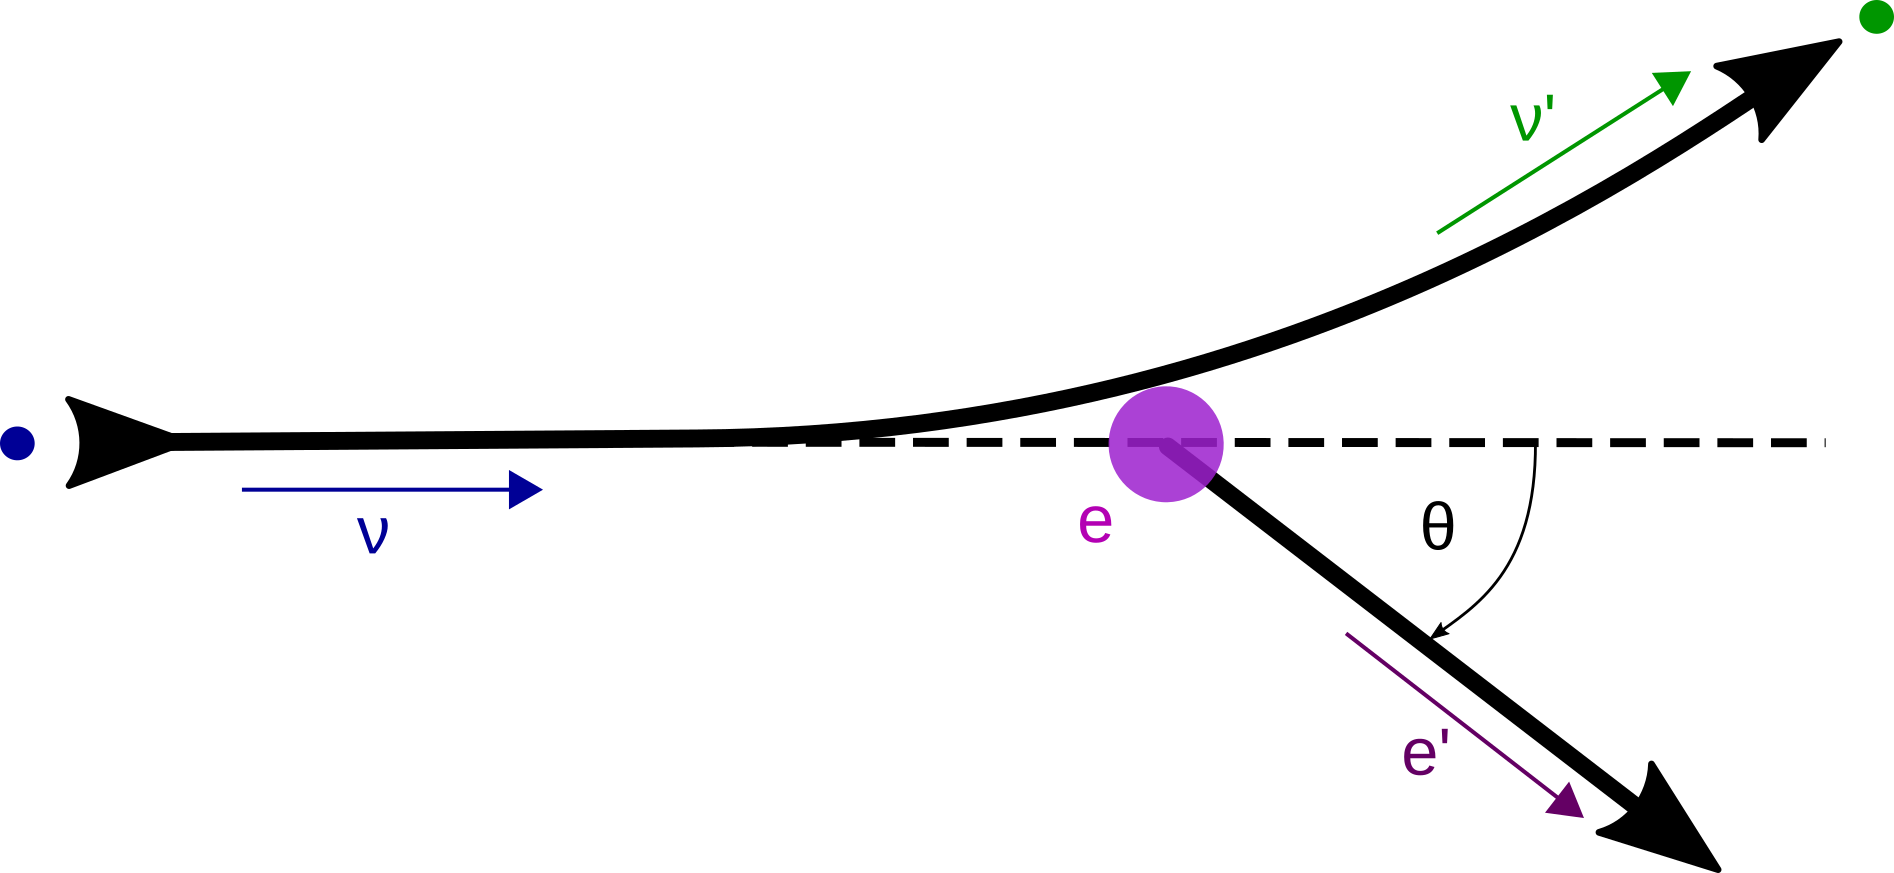
\includegraphics[width=0.55\linewidth]{Plots/NuMM/NuoneInteraction.png}
\caption{Neutrino-on-electron elastic scattering diagram}
\label{fig:NuoneDiagram}
\end{figure}

\note{Is this derivation too trivial to mention in a thesis? Should I just mention the results? I wanted to have this in the technote, but probably too detailed for a thesis...}
\todo{Also change all we to passive voice - or should I keep we here?}
From simple $2\rightarrow 2$ kinematics we can calculate
\begin{equation}
\left(P_{\nu}-P_{e^{\prime}}\right)^2=\left(P_{\nu^{\prime}}-P_e\right)^2,
\end{equation}
\begin{equation}
m_{\nu}^2+m_e^2-2E_{\nu}E_{e^{\prime}}+2E_{\nu}p_{e^{\prime}}\cos\theta=m_{\nu}^2+m_e^2-2E_{\nu^{\prime}}m_e.
\end{equation}
Using the energy conservation
\begin{equation}
E_{\nu}+m_e=E_{\nu^{\prime}}+E_{e^{\prime}}=E_{\nu^{\prime}}+T_e+m_e\Rightarrow E_{\nu^{\prime}}=E_{\nu}-T_e
\end{equation}
we get
\begin{equation}
E_{\nu}p_{e^{\prime}}\cos\theta=E_{\nu}E_{e^{\prime}}-E_{\nu^{\prime}}m_e=E_{\nu}\left(T_e+m_e\right)-\left(E_{\nu}-T_e\right)m_e=T_e\left(E_{\nu}+m_e\right),
\end{equation}
\begin{equation}
\cos\theta=\frac{E_{\nu}+m_e}{E_{\nu}}\sqrt{\frac{T_e^2}{E_{e^{\prime}}^2-m_e^2}}=\frac{E_{\nu}+m_e}{E_{\nu}}\sqrt{\frac{T_e^2}{T_e^2+2T_em_e}}.
\end{equation}
And finally we get
\begin{equation}\label{eq:ThetaTRelation}
\cos\theta=\frac{E_{\nu}+m_e}{E_{\nu}}\sqrt{\frac{T_e}{T_e+2m_e}}.
\end{equation}

We can rearrange the Eq.~\ref{eq:ThetaTRelation} to get
\begin{equation}\label{eq:TThetaRelation}
T_e=\frac{2m_eE_\nu^2\cos^2\theta}{\left(E_\nu+m_e\right)^2-E_\nu^2\cos^2\theta}.
\end{equation}
Electron's kinetic energy is therefore kinematically constrained by the energy conservation as
\begin{equation}
T_e\leq\frac{2E_{\nu}^2}{2E_{\nu}+m_e},
\end{equation}
which corresponds to the $\cos\theta\rightarrow 1$ when the recoil electron goes exactly forward in the incident neutrino direction.

Considering $E_{\nu}\sim\textsf{GeV}$, we can approximate $\frac{m_e^2}{E_{\nu}^2}\rightarrow 0$ and from Fig.\ref{fig:TThetaDistribution} we can see that we can approximate all recoil angles to be very small, therefore $\theta^2\cong \left(1-\cos^2\theta\right)$. Using Eq.\ref{eq:ThetaTRelation} we get
\begin{equation}
T_e\theta^2\cong T_e\left(1-\left(\frac{E_\nu+m_e}{E_\nu}\right)^2\frac{T_e}{T_e+2m_e}\right)
=T_e\left(1-\left(1+\frac{2m_e}{E_\nu}\right)\frac{T_e}{T_e+2m_e}\right),
\end{equation}
therefore
\begin{equation}
T_e\theta^2\cong \frac{2m_eT_e}{T_e+2m_e}\left(1-\frac{T_e}{E_\nu}\right)=2m_e\left(\frac{1}{1+\frac{2m_e}{T_e}}\right)\left(1-\frac{T_e}{E_\nu}\right),
\end{equation}
and finally
\begin{equation}\label{eqTThetaSqExp}
T_e\theta^2\cong 2m_e\left(1-\frac{T_e}{E_{\nu}}\right)<2m_e.
\end{equation}

This is a strong limit that clearly distinguishes the \gls{nuone} elastic scattering events from other similar interaction involving single electron (mainly the $\nu_e$\gls{CC} interaction).

\begin{figure}[hbtp]
\centering
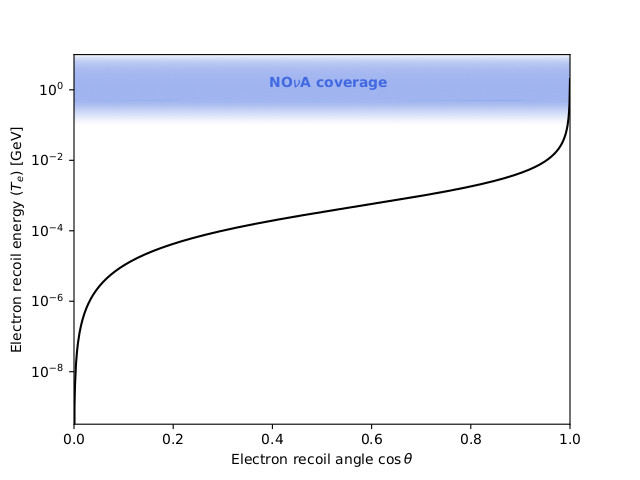
\includegraphics[width=.7\linewidth]{Plots/NuMM/KinematicsTOnTh.jpeg}
\caption[Electron recoil energy versus recoil angle]{Relation between the recoil electron's kinetic energy and angle for \acrshort{nuone} elastic scattering. The coverage of the \acrshort{NOvA} detectors for measuring the electron recoil energy is shown in blue. Only very forwards electron's are recorded in \acrshort{NOvA}.}
\label{fig:TThetaDistribution}
\end{figure}

\subsubsection{Neutrino magnetic moment cross section}
\note{Should this only be a subsubsection?}
In the ultra-relativistic limit, the neutrino magnetic moment changes the neutrino helicity, turning active neutrinos into sterile \todo{cite this properly}. Since the \gls{SM} weak interaction conserves helicity we can simply add the two contribution to the \gls{nuone} cross section incoherently \cite{nuElmagInt2015.pdf}:
\begin{equation}
\frac{d\sigma_{\nu_le^-}}{dT_e}=\left(\frac{d\sigma_{\nu_le^-}}{dT_e}\right)_{\textsf{SM}}+\left(\frac{d\sigma_{\nu_le^-}}{dT_e}\right)_{\textsf{MAG}}.
\end{equation}

The \gls{SM} contribution can be expressed as \cite{nuElmagInt2015.pdf}:
\begin{multline}
\left(\frac{d\sigma_{\nu_le^-}}{dT_e}\right)_{\textsf{SM}}=\frac{G_F^2m_e}{2\pi}\left\lbrace\left(g_V^{\nu_l}+g_A^{\nu_l}\right)^2+\left(g_V^{\nu_l}-g_A^{\nu_l}\right)^2\left(1-\frac{T_e}{E_{\nu}}\right)^2\right.\\
+\left.\left(\left(g_A^{\nu_l}\right)^2-\left(g_V^{\nu_l}\right)^2\right)\frac{m_eT_e}{E_{\nu}^2}\right\rbrace,
\end{multline}
where the coupling constants $g_V$ and $g_A$ are different for different neutrino flavours and for antineutrinos. Their values are:
\begin{align}
g_V^{\nu_e}&=2\sin^2\theta_W+1/2,\hspace{2.5cm} g_A^{\nu_e}=1/2,\\
g_V^{\nu_{\mu,\tau}}&=2\sin^2\theta_W-1/2,\hspace{2.25cm} g_A^{\nu_{\mu,\tau}}=-1/2.
\end{align}
For antineutrinos $g_A\rightarrow -g_A$.

\todo{Decide if this is actually useful or not}
Using Eq.~\ref{eq:TThetaRelation} it is possible to get the differential cross section for $\cos\theta$:
\begin{equation}
dT_e=\frac{4m_eE_\nu^2\left(m_e+E_\nu\right)^2}{\left[\left(m_e+E_\nu\right)^2-E_\nu^2\cos^2\theta\right]^2}\cos\theta d\cos\theta
\end{equation}
as
\begin{multline}
\left(\frac{d\sigma_{\nu_le^-}}{d\cos\theta}\right)_{\textsf{SM}}=
\frac{2G_F^2E_{\nu}^2m_e^2\cos\theta\left(E_{\nu}+m_e\right)^2}{\pi\left(\left(E_{\nu}+m_e\right)^2-E_{\nu}^2\cos^2\theta\right)^2}\\
\left\lbrace\left(g_V^{\nu_l}+g_A^{\nu_l}\right)^2+
\left(g_V^{\nu_l}-g_A^{\nu_l}\right)^2\left(1-\frac{2m_eE_{\nu}\cos^2\theta}{\left(E_{\nu}+m_e\right)^2-E_{\nu}^2\cos^2\theta}\right)^2\right.+\\
\left.\left(\left(g_A^{\nu_l}\right)^2-\left(g_V^{\nu_l}\right)^2\right)
\frac{2m_e^2\cos^2\theta}{\left(\left(E_{\nu}+m_e\right)^2-E_{\nu}^2\cos^2\theta\right)}\right\rbrace,
\end{multline}

\begin{table}{ht}
\centering
\caption{Neutrino-on-electron elastic scattering total cross sections. \todo{Move units to title and add cross sections with thresholds. Also reference this somewhere in text} from Fundamentals of neutrino Physics and Astrophysics, p.139}
\begin{tabular}{cc}
\hline
Process & Total cross section\\\hline
$\nu_e+e^-$ & $\simeq 93\times 10^{-43} E_\nu\unit{cm^2 GeV^{-1}}$\\
$\overline{\nu}_e+e^-$ & $\simeq \unit[39\times 10^{-43} E_\nu]{cm^2 GeV^{-1}}$\\
$\nu_{\mu,\tau}+e^-$ & $\simeq \unit[15\times 10^{-43} E_\nu]{cm^2 GeV^{-1}}$\\
$\overline{\nu}_{\mu,\tau}+e^-$ & $\simeq \unit[13\times 10^{-43} E_\nu]{cm^2 GeV^{-1}}$\\\hline
\end{tabular}
\end{table}

The neutrino magnetic moment contribution is \todo{include derivation from \cite{NeutrinoElmagFormFactors1989.pdf}} \cite{nuElmagInt2015.pdf}:
\begin{equation}
\left(\frac{d\sigma_{\nu_le^-}}{dT_e}\right)_{\textsf{MAG}}=\frac{\pi\alpha^2}{m_e^2}\left(\frac{1}{T_e}-\frac{1}{E_{\nu}}\right)\left(\frac{\mu_{\nu_l}}{\mu_B}\right)^2,
\end{equation}
where $\alpha$ is the fine structure constant \todo{Calculate the total mag moment cross sections}.

Comparison of the \gls{SM} and the neutrino magnetic moment cross sections is shown on Fig.\ref{fig:NuMMCrossSectionComparison}. Whereas the \gls{SM} cross section is flat with $T_e\rightarrow 0$, the neutrino magnetic moment cross section keeps increasing to infinity. However, this reach is limited by the experimental capabilities of detecting such low energetic neutrinos. Possible \gls{NOvA} coverage is shown in a shaded blue and it is uncertain we could actually reach as low as $100\ \unit{MeV}$ \todo{Change this claims a little bit}.

\begin{figure}[hbtp]
\centering
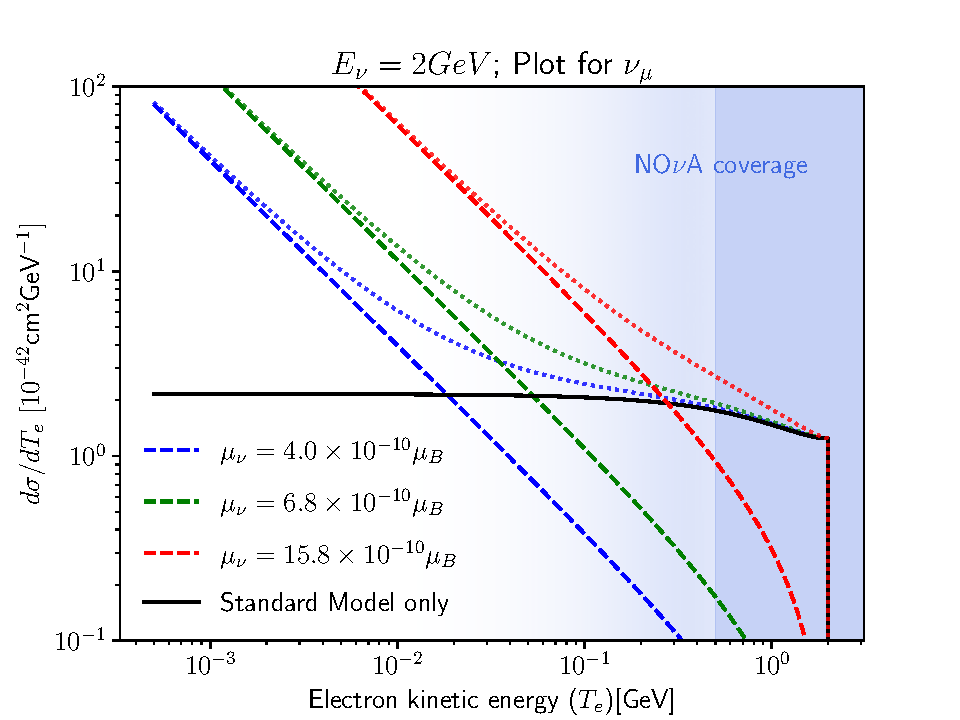
\includegraphics[width=.9\textwidth]{Plots/NuMM/dSdTNumuMMCompAltLim.pdf}
\caption[Comparison of the neutrino magnetic moment and Standard Model cross sections]{Comparison of the neutrino magnetic moment (coloured) and the \acrshort{SM} (black) cross sections for the \acrshort{nuone} elastic scattering. Different colours depict different values of the neutrino magnetic moment. Dashed lines are the individual cross sections and dotted lines are the added total cross section with the standard model contribution. \acrshort{NOvA} coverage of electron recoil energies is shown in shaded blue \todo{Reference the colours on the figures to the origins of the values (LSND and Biao)}.}
\label{fig:NuMMCrossSectionComparison}
\end{figure}

As can be seen in Fig.~\ref{fig:NuMMCrossSectionComparison} and Fig.~\ref{fig:NuMMCrossSectionRatios}, the magnetic moment contribution exceeds the \gls{SM} contribution for low enough $T_e$. This can be approximated as \cite{nuElmagInt2015.pdf}:
\begin{equation}
T_e\lesssim\frac{\pi^2\alpha^2}{G_F^2m_e^3}\left(\frac{\mu_{\nu}}{\mu_B}\right)^2\simeq 2.9\times 10^{19}\left(\frac{\mu_{\nu}}{\mu_B}\right)^2\left[\textsf{MeV}\right],
\end{equation}
which does not depend on the neutrino energy and makes experiments sensitive to lower energetic electrons more sensitive to the neutrino magnetic moment. This is especially true for the recent dark matter experiments which put stringent limits on the solar neutrino effective magnetic moment, as described in the following section.

\begin{figure}[hbtp]
\centering
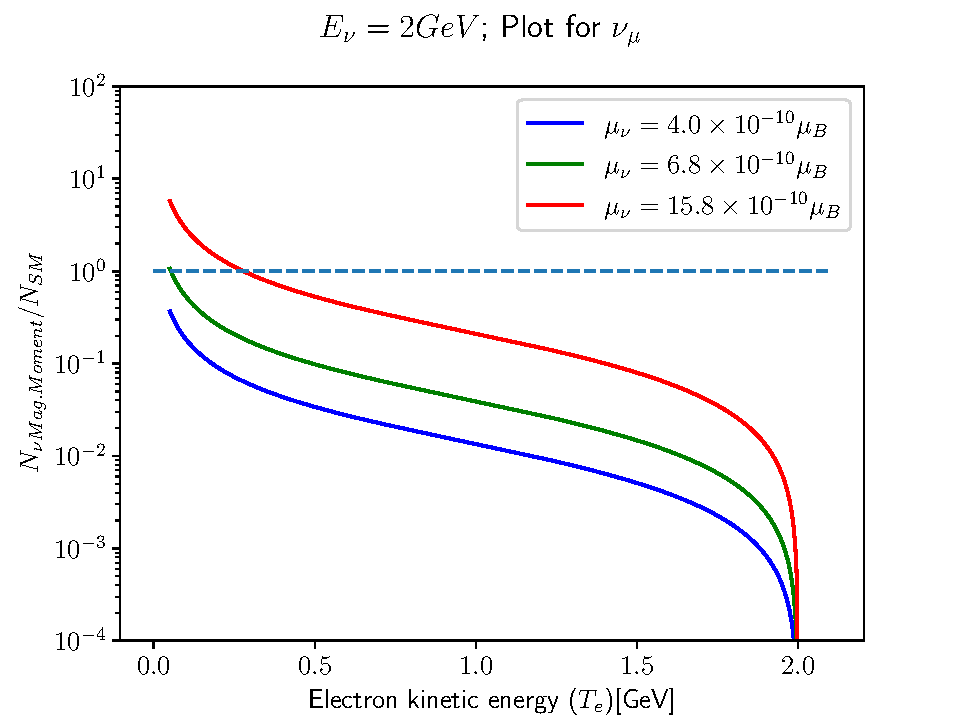
\includegraphics[width=.9\textwidth]{Plots/NuMM/RatioNumuMMCompLinX.pdf}
\caption[Ratio of the neutrino magnetic moment and Standard Model cross sections]{Ratio of the neutrino magnetic moment cross section to the \acrshort{SM} cross section for the \acrshort{nuone} elastic scattering. Different colours depict different effective muon neutrino magnetic moment values.}
\label{fig:NuMMCrossSectionRatios}
\end{figure}

%%%%%%%%%%%%%%%%%%%%%%%%%%%%%%%%%%%%%%%%%%%%%%%%%%%%%%%%%%%%%%%%%%%%%
%%%                       ANALYSIS OVERVIEW                       %%%
%%%%%%%%%%%%%%%%%%%%%%%%%%%%%%%%%%%%%%%%%%%%%%%%%%%%%%%%%%%%%%%%%%%%%
\section{Analysis overview}\label{sec:NuMMAnalysisOverview}

Our analysis strategy is to compare the count of the recorded neutrino events in data with the prediction. The prediction consists of the signal, which is directly related to the value of the neutrino magnetic moment, and the background, which corresponds to the predicted events under the \gls{SM}. The signal is defined as true \gls{nuone} events with the neutrino magnetic moment cross section instead of the \gls{SM} one. Additionally, we require the true vertex to be contained inside of the \gls{ND} to remove events that originates from outside of the detector. Background is everything else.

The data used in this analysis was collected from the start of the \gls{NOvA} \gls{ND} data taking on the 22$^{\textsf{nd}}$ of August 2014, until the 3$^{\textsf{rd}}$ of February 2021. This is the \gls{ND} data that was used in the latest \gls{NOvA} neutrino oscillations result \cite{NOvAResults2021.pdf}, with an additional one year of data taking. The \gls{ND} collected more data since February 2021 which is however still being processed and it is not available at the time of writing this thesis. The full \gls{ND}-equivalent exposure of the data sample is approximately $13.8\times10^{20}$~\gls{POT}. This exposure is used throughout the rest of this chapter to scale the predicted distributions and number of events. \note{Should I also talk about the RHC sample here? Future data?}

Maybe also mention something about the data that was excluded - bad runs and bad channels?

This analysis uses the standard \gls{NOvA} simulation and reconstruction tools, as were discussed in Sec.~\ref{sec:NOvASimulation} and \ref{sec:NOvAReconstruction}. The simulation was created with approximately $4\times$ larger statistics than is available in data to limit statistical uncertainties from simulation. The total exposure for the simulation is approximately $55.4\times10^{20}$~\gls{POT}. However, for the studies of the systematic uncertainties, only a smaller portion of this full sample is used, specifically $19.3\times10^{20}$~\gls{POT} \gls{ND}-equivalent.

%Analysis weights - PPFX and cross section
The corrections for the known limitations in the simulation are applied in the form of event-by-event analysis weights, which weight each single event based on how it is affected by that particular variation in simulation. To correct for known deficiencies in simulation of neutrino flux or cross sections we apply weights calculated for each event. This includes the external measurements that correct the neutrino beam prediction inside \gls{PPFX} as described in Sec.~\ref{sec:NOvASimulation}, and for the non-\gls{nuone} background, also the internal and external measurements that constrain the neutrino interaction prediction inside GENIE. These are not applied to the \gls{nuone} events, as they are assumed to be known precisely from theory.  However, the GENIE \gls{MC} simulation doesn't consider radiative corrections for the \gls{nuone} events, which are however trivial to implement.

%Radiative correction weight
Mention here where did I get the original GENIE cross section from (reference Yiwen's talk or technote, plus the original paper that was used). nu-on-e technote\cite{NOVA-doc-56383}

\todo{Write out the actual version of the weight. Including the original and the corrected XSec constants}

MINERvA paper \cite{MinervaNuoneFluxConstraint2019.pdf}: At tree level, the neutrino-electron scattering cross section is given by... (basically same as I have in the theory) corrected for updated electroweak couplings, CLL and CLR [17] and one-loop electroweak radiative corrections as calculated in Ref. [18]. One deficiency of the calculation of Ref. [18] is that it does not contain the term in the one-loop cross section proportional to CLL CLR. This deficiency is corrected in a recent calculation [38], and that result is given below. However, as illustrated in Eq. (A1) this term also contains an additional power of m/Enu compared to the terms proportional to C2 LL and C2 LR, and the entire term is therefore negligible at the few-GeV neutrino energies of the MINERvA experiment.
%[17] is https://www.sciencedirect.com/science/article/pii/S0146641013000239?via%3Dihub \cite{NuoneRadCorrConstants2013.pdf}
%[18] is https://www.sciencedirect.com/science/article/pii/0550321384902931?via%3Dihub \cite{NuoneRadCorrEquation1984.pdf}

Say that we are not using the third part of the correction because it is tiny and it makes no difference. (tried and tested)

[ND group's technote] In GENIE, the cross section of the nuone elastic scattering signal is calculated at the tree level. To improve the precision of the simulated nuone elastic scattering cross section, we performed radiative corrections to the GENIE nuone elastic scattering as shown in Appendix A. The precision of the simulated nuone elastic scattering cross section is improved by tuning CLL and CLR to one-loop values obtained from global fits to electroweak data 14 and 2. The radiative correction also includes additional low-energy terms in the expression of differential cross section of nuone elastic scattering. In comparison, the neutrino interactions in the NOvA detector are simulated using the GENIE neutrino event generator, where the Weinberg Angle is 0.501716712132. After radiative corrections, the total number of nuone elastic scattering increases  0.83\% from the standard GENIE MC.

\todo{correct the equation}
Calculated as 
\begin{equation}
weight_{\text{Radiative Corr.}} = \left.\frac{d\sigma_{\nu-on-e}}{dy}\right|_{\text{Radiative Corr.}} / \left.\frac{\textsf{d}\sigma_{\nu-on-e}}{\textsf{d}y}\right|_{\text{GENIE 3}};\,y=\frac{E_e-m_e}{E_\nu}
\end{equation}

\iffalse
For the GENIE constants I use
    double C_LL, C_LR;                                                                                                                                             
    if (pdg == 14) {                                                                                                                                               
      C_LL = -0.268705;                                                                                                                                            
      C_LR =  0.231295;                                                                                                                                            
    } else if (pdg == -14) {                                                                                                                                       
      C_LL =  0.231295;                                                                                                                                            
      C_LR = -0.268705;                                                                                                                                            
    } else if (pdg == +12) {                                                                                                                                       
      C_LL = 0.731295;                                                                                                                                             
      C_LR = 0.231295;                                                                                                                                             
    } else if (pdg == -12) {                                                                                                                                       
      C_LL = 0.231295;                                                                                                                                             
      C_LR = 0.731295;                                                                                                                                             
    } else return 1.;                                                                                                                                              
                                                                                                                                                                   
    SMXSec *= pow(C_LL,2) + pow(C_LR,2)*pow(1-y,2) -                                                                                                               
              C_LL*C_LR*M_e*y/NuE;

And for radiative corrections:
    double C_LL, C_LR;                                                                                                                                             
    if (pdg == 14) {                                                                                                                                               
      C_LL = -0.2730;                                                                                                                                              
      C_LR =  0.2334;                                                                                                                                              
    } else if (pdg == -14) {                                                                                                                                       
      C_LL =  0.2334;                                                                                                                                              
      C_LR = -0.2730;                                                                                                                                              
    } else if (pdg == +12) {                                                                                                                                       
      C_LL = 0.7276;                                                                                                                                               
      C_LR = 0.2334;                                                                                                                                               
    } else if (pdg == -12) {                                                                                                                                       
      C_LL = 0.2334;                                                                                                                                               
      C_LR = 0.7276;                                                                                                                                               
    } else return 1.;
    
    double X1 = -2.*log(2.*y*NuE/M_e)/3. + pow(y,2)/24. - 5.*y/12. -                                                                                               
                pow(PI,2)/6. + 23./72.;                                                                                                                            
    double X2 = -2.*log(2.*y*NuE/M_e)/3. - pow(y,2)/(18.*pow(1-y,2)) -                                                                                             
                pow(PI,2)/6. - 2.*y/(9.*pow(1-y,2)) + 23./(72.*pow(1-y,2));                                                                                        
                                                                                                                                                                   
    RCXSec *= pow(C_LL,2)*(1+alpha*X1/PI) +                                                                                                                        
              pow(C_LR,2)*pow(1-y,2)*(1+alpha*X2/PI) -                                                                                                             
              (C_LL*C_LR*M_e*y/NuE);
\fi


%Magnetic moment as a weight 
\todo{What does this do and why does it work? Reference the theory part as to why is the magnetic moment signal simply a rescaling of the GENIE cross section.}

Using the same tree-level cross section from GENIE as in the rad. corr. weight.

\todo{Write the name of the weight in CAFAna/nuone namespace and where it is located}

\todo{correct the equation}
Calculated as 
\begin{equation}
weight_{\nu\text{ Mag. Moment}} = \left.\frac{d\sigma_{\nu-on-e}}{dy}\right|_{\nu\text{ Mag. Moment}} / \left.\frac{\textsf{d}\sigma_{\nu-on-e}}{\textsf{d}y}\right|_{\text{GENIE 3}};\,y=\frac{E_e-m_e}{E_\nu}
\end{equation}

%Enhanced nuone sample
Due to the relatively low cross section of the \gls{nuone} interaction, the nominal simulation sample contains too few \gls{nuone} events, which could result in a significant statistical uncertainty from simulation. To avoid this, we created a \gls{nuone}-enhanced simulation sample which contains mainly \gls{nuone} events with a little non-\gls{nuone} background overlaid on top to properly account for the possible reconstruction effects of the pileup of neutrino interactions in one spill \cite{NOVA-doc-56383}. In the real detector, the hits from the true \gls{nuone} interaction can be clustered to another interaction, or additional hits can be clustered together into the \gls{nuone} event. The total exposure of the \gls{nuone}-enhanced sample is $1.72\times10^{24}$~\gls{POT}. To save up on unnecessary disk space and processing usage, the enhanced \gls{nuone} sample does not include any cross section related parameters and variables, as the \gls{nuone} interaction is assumed to be known exactly from theory.

%[ND group's technote] Because the cross section of the nuone elastic scattering is very low (approx. 1/2000 of the total charged-current cross section), the statistics of nuone elastic scattering is not enough in the inclusive sample. In order to optimize the signal selection criteria, we made a sample with only nuone elastic scattering events in the detector. The size of this nuone signal MC is 1.48E23 POT. However the pile-up of neutrino interactions in one spill impacts on the hit clustering in reconstruction, either hits from the nuone elastic scattering can be clustered to other interactions or extra hits can be clustered to the nuone elastic scattering.

% enhanced nueccmec
The cross section tuning procedure in \gls{NOvA} (Sec.~\ref{sec:NOvASimulation}) applies large weights to \gls{MEC} events in some parts of the parameter space. However, after the full event selection described below in Sec.~\ref{sec:NuMMEventSelection} there is only a small amount of \gls{MEC} events, specifically $\nu_e$\gls{CC} \gls{MEC} events, left in the detector. Applying large tuning corrections to only a small number of events results in large statistical fluctuations. To avoid this, we created another special sample with enhanced number of $\nu_e$\gls{CC} \gls{MEC} events. We followed the same procedure as for the \gls{nuone}-enhanced sample, resulting in the final exposure of $1.99\times10^{24}$~\gls{POT}.

%Created by Yiwen Xiao \cite{NOVA-doc-56383} to tackle the low statistics of the $\nu_e$CC MEC background events and subsequently large and unphysical cross section weights. Correct POT is 1.99e+24 (filematched). There are limitations of the sample in the q3-q0 parameter space.

%[ND group's technote] After implementing GSF Xsec weights, the shape of background after selection shows multiple spikes from nue CC events.  Since the number of nue CC MEC events remained in the final sample is small, events with very large weight can distort the distribution of nue CC MEC events. In order to mitigate the effect for nue CC MEC events in the signal and sideband region (ETh2 < 0.04 GeV Rad2), a special nue CC MEC sample is produced with enlarged statistics. The nue CC MEC events after all selection in Production 5.1 MC are replaced by the nue CC MEC events in the special sample in the sections of DATA analysis and Systematic Uncertainty.

\iffalse
NOvAReweight reference: J. Wolcott, “NOvARwgt software.” https://github.com/novaexperiment/NOvARwgt-public.
[ND group's technote] The cross-section weight is a combination of different weights applied to various processes. The major effects of this weight are
\begin{itemize}
\item  Adjust the axial mass (MA) for CCQE cross section to $\unit[1.04]{GeV/c^2}$ based on the error-weighted mean of updated ANL, BNL, and FNAL experiments.
\item Applies the empirical MEC weight determined from the cross section tuning fit.
\item Reduces non-resonant single pion production by 50\%.
\item Applies RPA suppression that models nuclear screen effects at low values Q2 to QE and RES interactions.
\item Reduces GENIE predicted DIS events with $W>\unit[1.7]{GeV}$ by 10\%.
\end{itemize}
\fi


The summary of the simulation samples and analysis weights for the three different types of signal and background component is shown in Tab.~\ref{tab:NuMMSamplesAndWeightsOverview}.

\begin{table}[!ht]
\centering
\caption{Overview of the simulation samples and analysis weight used for the different signal and background components.}
\def\arraystretch{1.4}
\begin{tabular}{l@{\hskip 1cm}l@{\hskip 1cm}l}
Signal type            & Sample               & Weight\\\hline
Signal                 & Enhanced \gls{nuone} & Flux \& $\nu$ Mag. Moment\\
\gls{nuone} background & Enhanced \gls{nuone} & Flux \& Rad. Corr.\\
$\nu_e$\gls{CC} \gls{MEC} background & Enhanced $\nu_e$\gls{CC} \gls{MEC} & Flux \& Cross Sec.\\
Other background       & Nominal \gls{ND}     & Flux \& Cross Sec.
\end{tabular}
\label{tab:NuMMSamplesAndWeightsOverview}
\end{table}

%%%%%%%%%%%%%%%%%%%%%%%%%%%%%%%%%%%%%%%%%%%%%%%%%%%%%%%%%%%%%%%%%%%%%
%%%                         EVENT SELECTION                       %%%
%%%%%%%%%%%%%%%%%%%%%%%%%%%%%%%%%%%%%%%%%%%%%%%%%%%%%%%%%%%%%%%%%%%%%
\section{Event selection}\label{sec:NuMMEventSelection}
%Introduction:
We are searching for \gls{nuone} elastic scattering events, characterised by a single very forward going electron shower, specifically focusing on low electron recoil energies. The main background for our analysis come from $\nu_e$\gls{CC} interactions, which produce electron with an additional activity, and interactions that produce $\pi^0$, which decays into two photons producing electromagnetic showers, where each can look similar to the \gls{nuone} signal. Additionally, there are $\nu_\mu$\gls{CC} interactions, which are generally easy to identify from our signal, however their very high abundance in the \gls{NOvA} \gls{ND} makes them a dominant background nevertheless.

We explain the motivation behind each cut of the event selection and discuss their effect on the neutrino magnetic moment events below. We also consider possible improvements to the event selection for a future (re-)analysis.

The strategy for event selection is as follows. First, we remove events that failed reconstruction or data collection. Then, we apply pre-selection cuts that remove obvious background. The exact cut is selected by limiting the reduction of the signal efficiency to about $\unit[0.25]{\%}$. Following this, we apply the containment cuts that remove events that are either not fully contained within the detector, or events that originate from outside of the detector, such are rock muons. Afterwards, we consider several variables that could be used for the signal selection and evaluate their combined performance for a signal selection. We choose cut values that result in the best statistical significance, based on a chosen \gls{FOM}. Given that we are searching for a very limited number of signal events on top of a large background, we chose a simple statistics-only \gls{FOM}
\begin{equation}
\textsf{\gls{FOM}} = \frac{\textsf{Signal}}{\sqrt{\textsf{Background}}}.
\end{equation}

The summary of the cut values for the event selection of neutrino magnetic moment signal is presented in Tab.~\ref{tab:EventSelectionSummary}, showing the label for the event selection variable, its description and the cut value chosen. These event selection in total reduces signal $\unit[44.51]{\%}$, \gls{nuone} background $\unit[70.40]{\%}$ and other background $\unit[99.97]{\%}$. After the full event selection, the predicted number of signal events for $\mu_\nu=10^{-9}\mu_B$ is $23.31$ and the total number of background events under the \gls{SM} hypothesis is $678.26$. The most likely improvement is in probing the low energetic events and making sure they make sense. Additionally, it is possible to use a specially designed control regions to mitigate the very high non-\gls{nuone} background.

%[ND group's technote] Due to its small cross section, nuone elastic scattering contributes a small portion to the neutrino interactions happened in the detector. This section presents a thorough study regarding the features that can be utilized to differentiate nuone elastic scattering from other neutrino interactions. With the series of selection cuts, a sample with concentrated signals and strongly suppressed backgrounds is obtained in the ETh2 phase space.

\begin{table}[!hb]
\centering
\caption[Event selection summary]{Summary of the cut values for the event selection of neutrino magnetic moment signal showing the label for the event selection variable, its description and the cut value chosen. \note{Should I include the loose cuts here even when they were made stricter during TMVA?}}
\begin{tabular}{|m{0.2\textwidth} m{0.55\textwidth} m{0.15\textwidth}|}\hline
\textbf{Label} & \textbf{Description} & \textbf{Cut} \\\hline
\textbf{Valid Vtx} & Valid reconstructed vertex & $>0$\\
\textbf{N$^o$ Prongs} & Number of reconstructed prongs & $>0$\\
\textbf{Hits / Plane} & Number of hits per plane & $<5$\\\hline
\textbf{Low $E_{Shower}$} & Low cut on calorimetric energy of the most energetic shower & $>\unit[0.5]{GeV}$\\
\textbf{N$^o$ Hits Loose} & Preliminary cut on the total number of hits for all prongs in a slice & $<200$\\
\textbf{Prong Length} & Length of the longest prong & $<\unit[540]{cm}$\\
\textbf{$E\theta^2$ Loose} & Preliminary cut on the product of the calorimetric energy and angle squared of the leading shower & $<0.05$ $\unit{GeV\times rad^2}$\\
\textbf{High $E_{Shower}$ Loose} & Preliminary upper cut on the calorimetric energy of the most energetic shower & $<\unit[5.5]{GeV}$\\\hline
\multirow{6}{*}{\textbf{Fiducial}} & Vertex x position & $>\unit[-177]{cm}$ $<\unit[177]{cm}$\\
 & Vertex y position & $>\unit[-177]{cm}$ $<\unit[177]{cm}$\\
 & Vertex z position & $\unit[>50]{cm}$ $\unit[<1050]{cm}$\\\hline
\multirow{6}{*}{\textbf{Containment}} & Minimum hit position in x & $>\unit[-177]{cm}$\\
 & Maximum hit position in x & $<\unit[177]{cm}$\\
 & Minimum hit position in y & $>\unit[-185]{cm}$\\
 & Maximum hit position in y & $<\unit[177]{cm}$\\
 & Minimum hit position in z & $>\unit[55]{cm}$\\
 & Maximum hit position in z & $<\unit[1270]{cm}$\\\hline
\textbf{$E_{Shower}/E_{Tot}$} & Fraction of energy contained in the most energetic shower & $>0.91$\\
\textbf{N$^o$ Hits} & Total number of hits for all prongs in a slice & $<116$\\
\textbf{High $E_{Shower}$} & Calorimetric energy of the most energetic shower & $<\unit[1.4]{GeV}$\\
\textbf{\gls{nuone} ID} & \gls{CVN}-based \gls{nuone} identifier & $>0.65$\\
\textbf{$E\pi^0$ ID} & \gls{CVN}-based \gls{nuone} and $\pi^0$ identifier & $>0.63$\\
\textbf{$E\theta^2$} & Product of the calorimetric energy and angle squared of the leading shower & $<0.0048$ $\unit{GeV\times rad^2}$\\\hline
\end{tabular}
\label{tab:EventSelectionSummary}
\end{table}

\subsection{Data Collection Quality}
To ensure good data quality, we apply the following criteria to data only. These involve the the spill time cut, at least $2\time10^{12}$ \gls{POT} per spill, the current in the focusing horn within $\unit[-202]{kA}<I_{Horn}<\unit[-196.4]{kA}$, position of the beam is within $\pm\unit[2]{cm}$ in both x and y axis and that the width of the beam is within $0.57$ and $\unit[1.58]{cm}$. Additionally, we remove events that are incomplete, or with problems in one or more \glspl{DCM}. \todo{Reference the 3f data quality technote}

\subsection{Reconstruction Quality}

Since electron are reconstructed by slicing, then vertexing, then reconstructing prongs. To identify electron we request that there is a valid reconstructed vertex and at least one reconstructed prong. Even though electrons only consist of a single shower, we don't reject events with more than one prongs in a slice, as the reconstruction can wrongly assign noise hits as a separate prong. We do not want to reject these events as we might still recover the true signal event from there.

Figure~\ref{fig:NuMMCutsVertexIsValid} and Tab.~\ref{tab:CutflowTableBasicRecoQC} show that about $\unit[67]{\%}$ signal events do not have a valid reconstructed vertex. This is due to the concentration of the signal events at very low electron recoil energies, which can often consist of a single hit or only a few hits. As can be seen in the bottom plot of Fig.~\ref{fig:NuMMCutsVertexIsValid}, events with small true electron recoil energy have much smaller vertex reconstruction efficiency than higher energetic electrons. However, improving \gls{NOvA} vertex reconstruction at low energies might significantly aid the search for the neutrino magnetic moment. Ongoing work is improving the vertex reconstruction by using \gls{ML} approach instead of the currently used Hough transform together with Elastic Arms \cite{NOvA-doc-61190}.

\begin{figure}[hbtp]
\centering
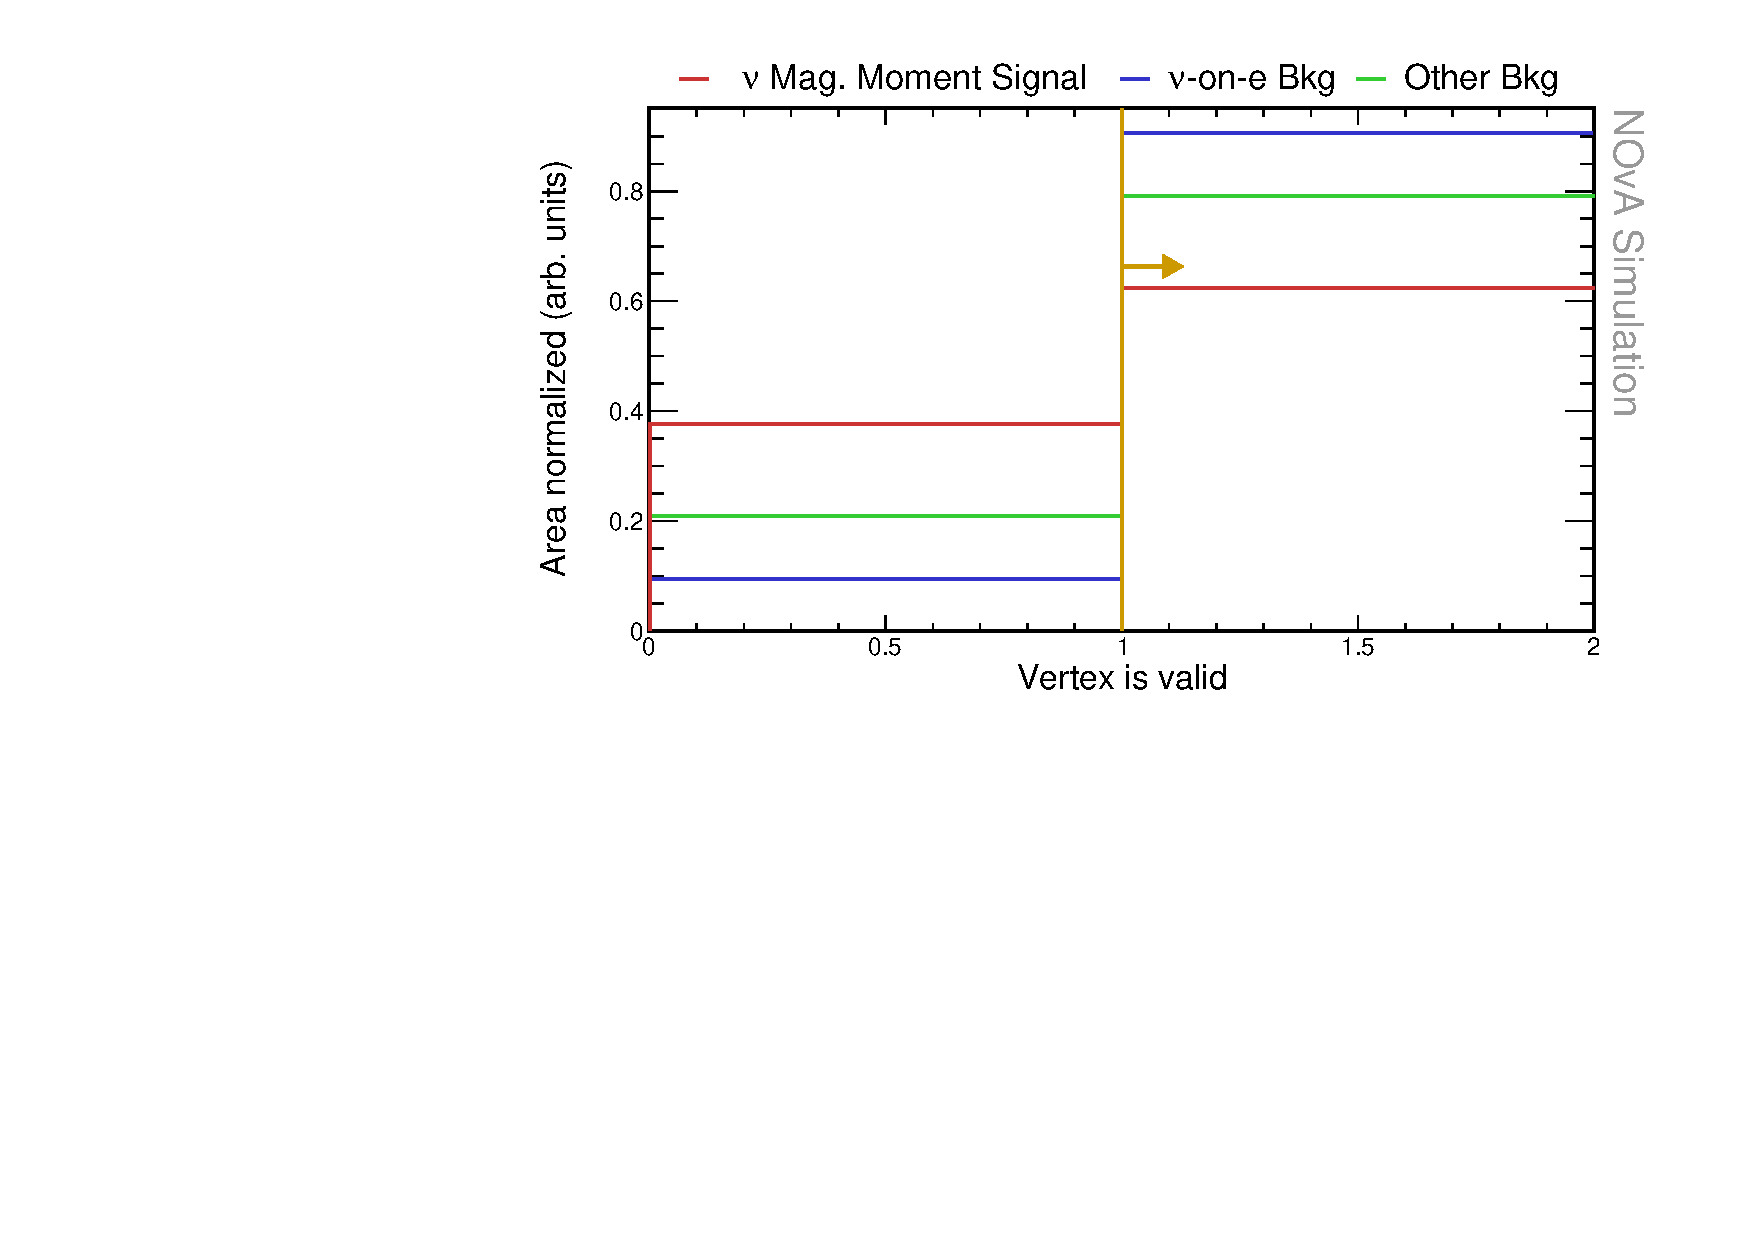
\includegraphics[width=.9\textwidth]{Plots/NuMMEventSelection/N1Cut_vtxIsValid.pdf}
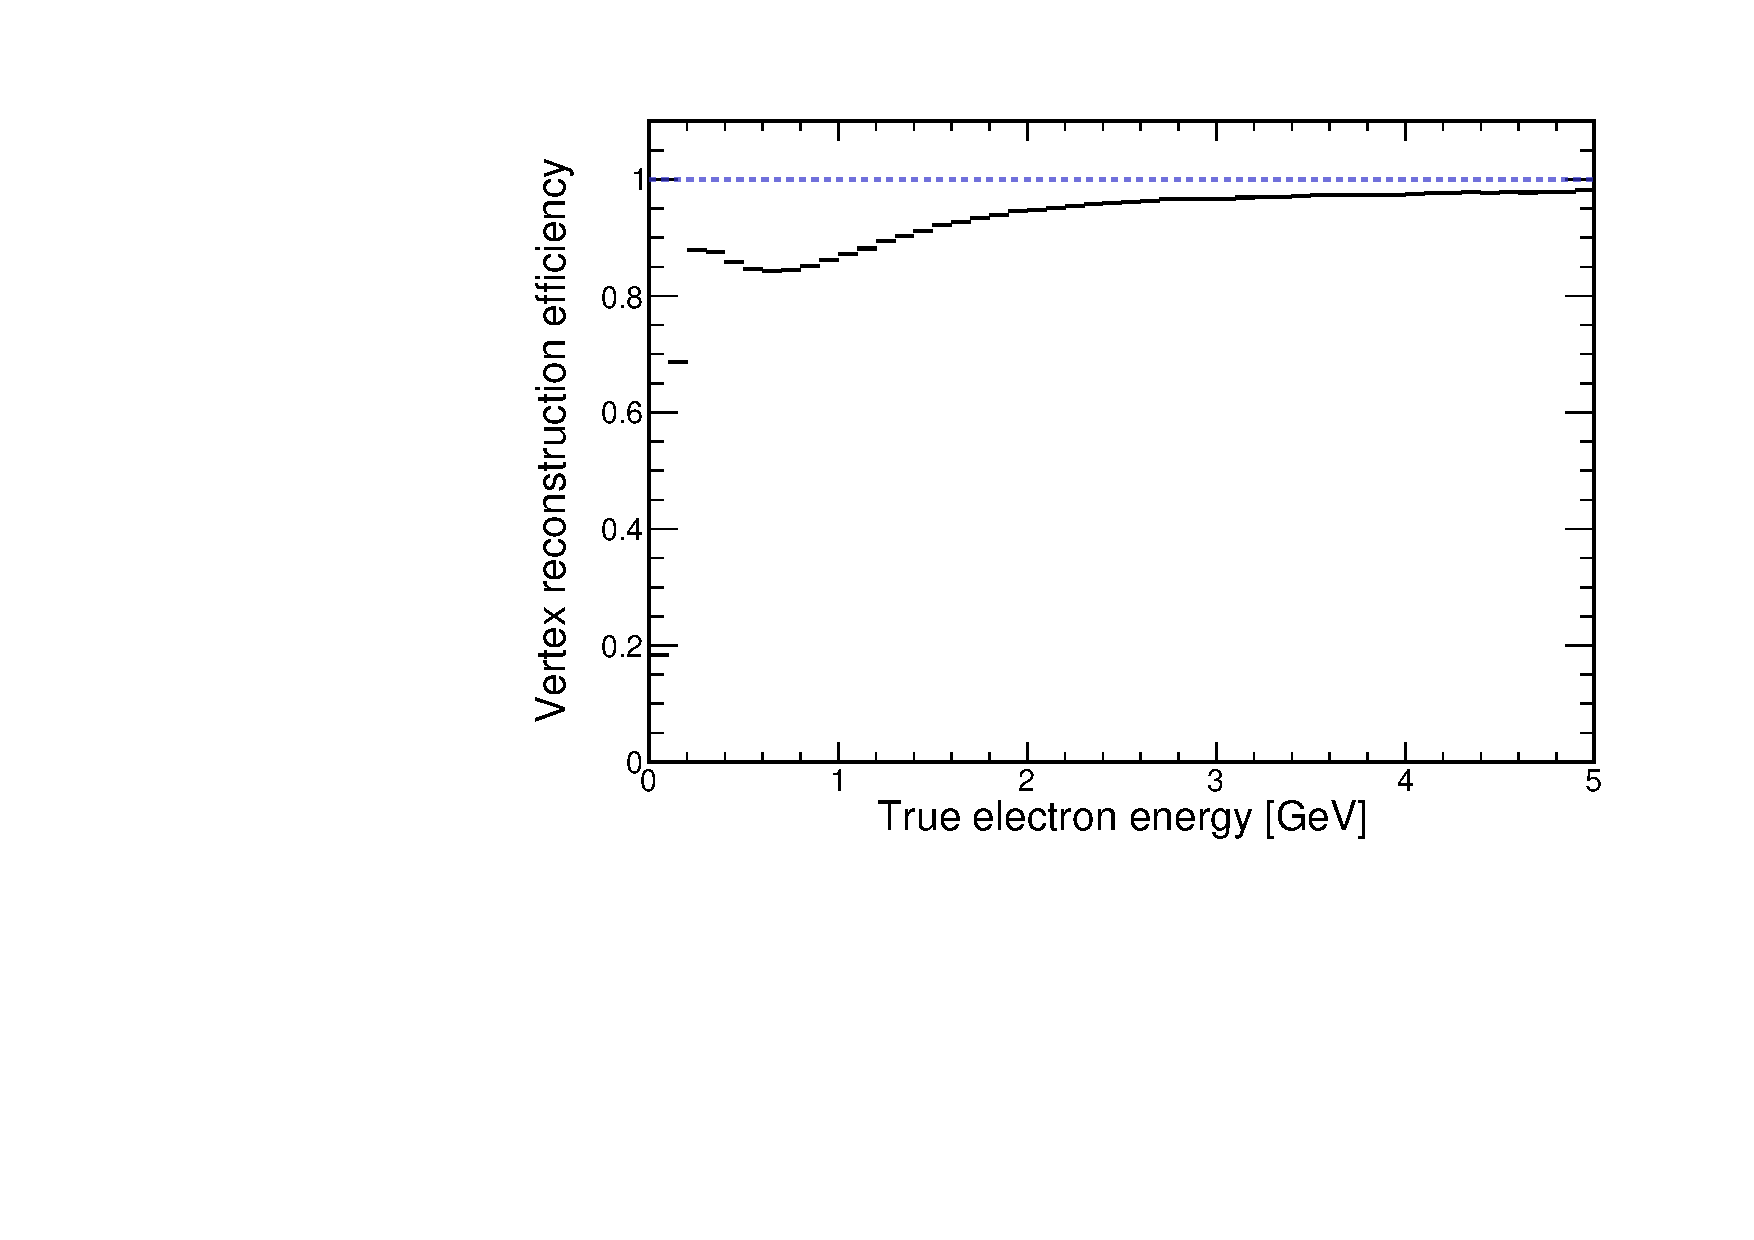
\includegraphics[width=.9\textwidth]{Plots/NuMMEventSelection/VtxIsValidNuMM.pdf}
\caption[Vertex reconstruction quality cut]{Top: Relative comparison of the signal (red), \acrshort{nuone} background (blue), and other background (green) events for the vertex reconstruction quality selection. Each histogram is area-normalised and the first bin corresponds to events without a valid vertex and second bin to events with correctly reconstructed vertex. The yellow line indicates the chosen cut value: all events have to have a valid reconstructed vertex. Bottom: profile histogram of the `vertex is valid' variable as a function of the true electron energy for the true signal events, showing the significant drop in vertex reconstruction efficiency at low electron recoil energies. No selection was applied prior to making these plots.}
\label{fig:NuMMCutsVertexIsValid}
\end{figure}

Additionally, we're placing a cut on the number of hits per plane to $<5$. This is to remove the so-called `\gls{FEB} flashers', which are caused by a very high energy deposit in one cell, such that it affects all the other channel on the same \gls{APD} \cite{NOvA-doc-37668}. The cut value was chosen so that it removes $\leq\unit[0.25]{\%}$ signal events, which is the same criterion as is used for the basic event selection cuts described below. Relative comparisons between signal and background for the number of prongs and the number of hits per plane are shown in Fig.~\ref{fig:NuMMCutsRecoQuality}.

%In pre-selection we also include a cut on the time difference between the mean times of the "current" slice and of the slice closest in time, which should be $>25\ \unit{ns}$. This ensures that ... \todo{This is to remove slicing failures that split the two gamma from a $\pi^0$ into two slices that resemble electron signal. Should we remove them now though?}.

%[nueXSec ana, docdb:37668] One additional detector issues is the presence of "FEB Flashers" within reconstructed slices. FEB flashers are caused by high  energy deposits in one cell, which induces a sagged baseline in all other channels on the same APD. When the baseline is restored, fake hits are triggered on the whole APD.

\begin{figure}[hbtp]
\centering
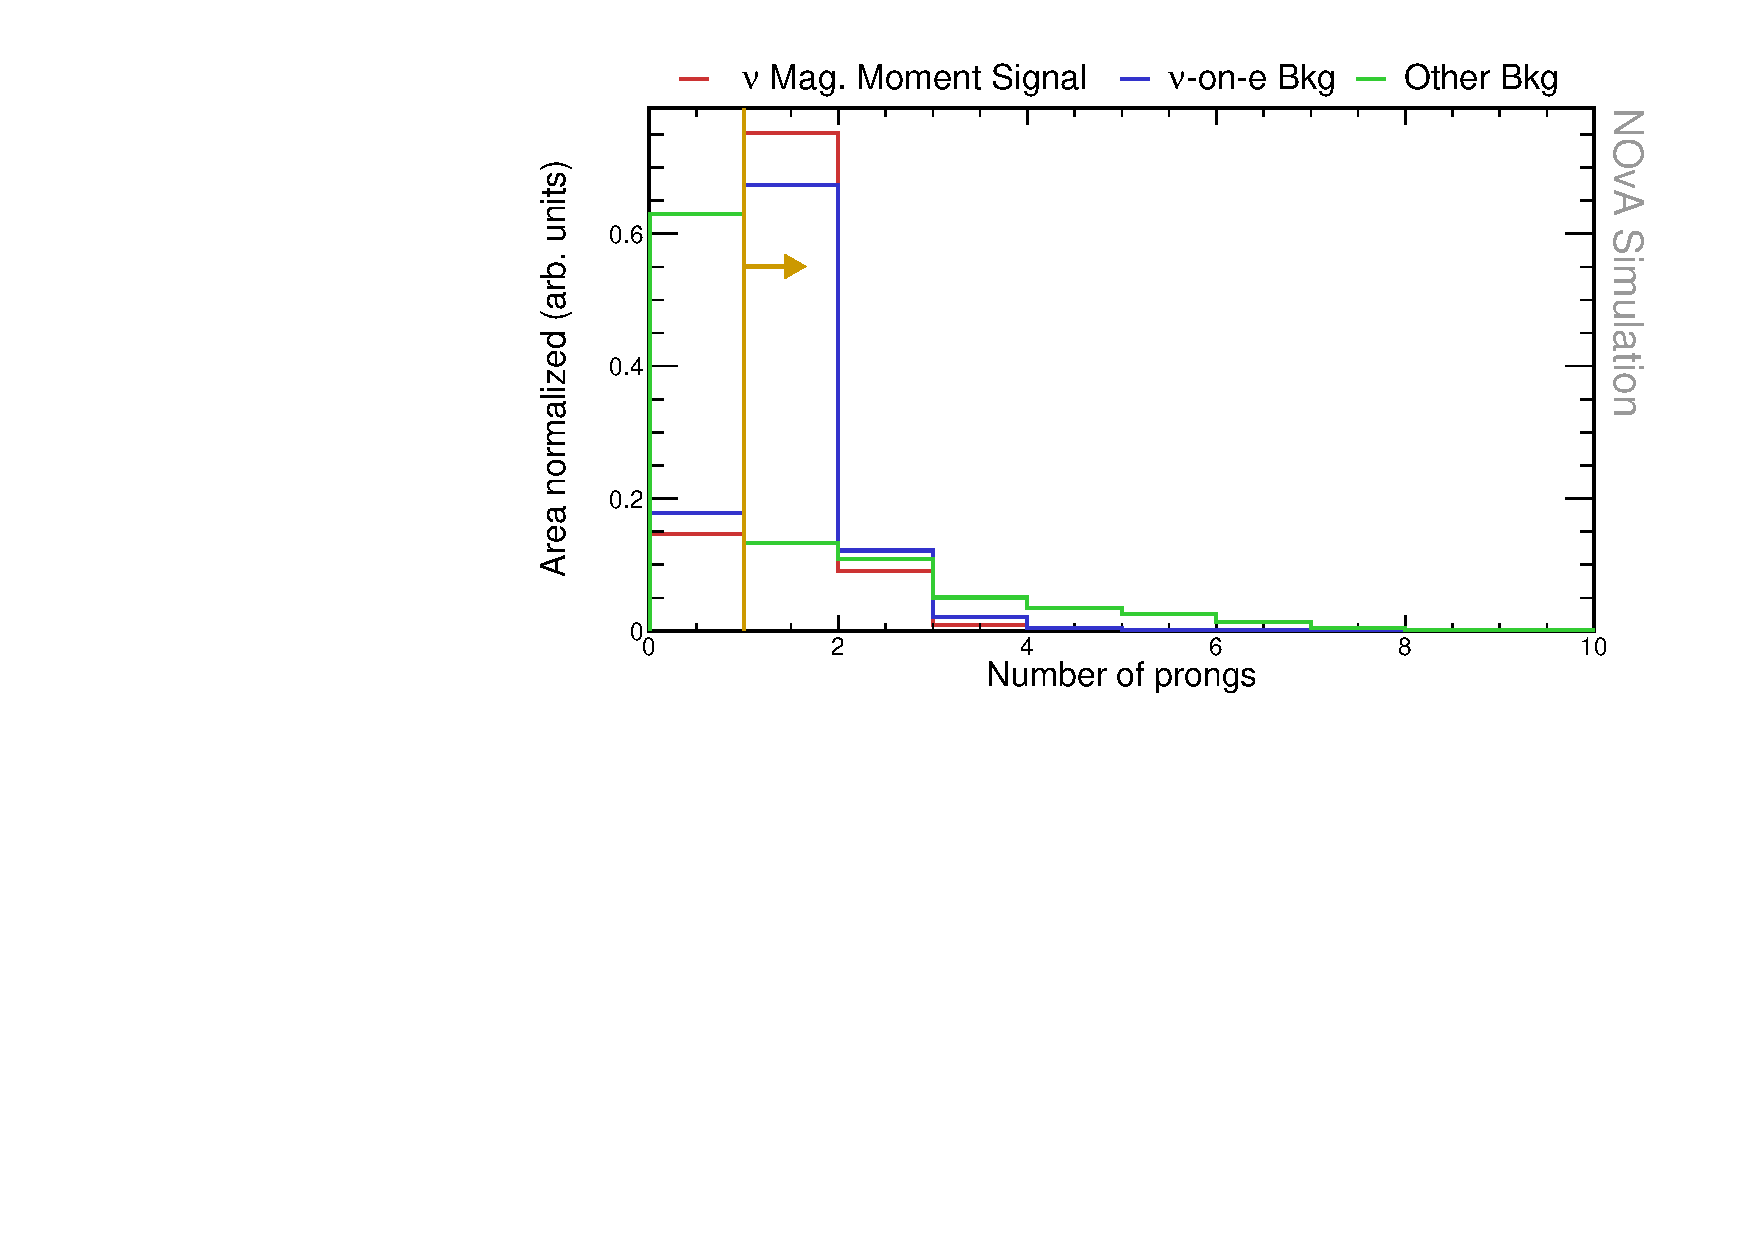
\includegraphics[width=.9\textwidth]{Plots/NuMMEventSelection/N1Cut_NPng.pdf}
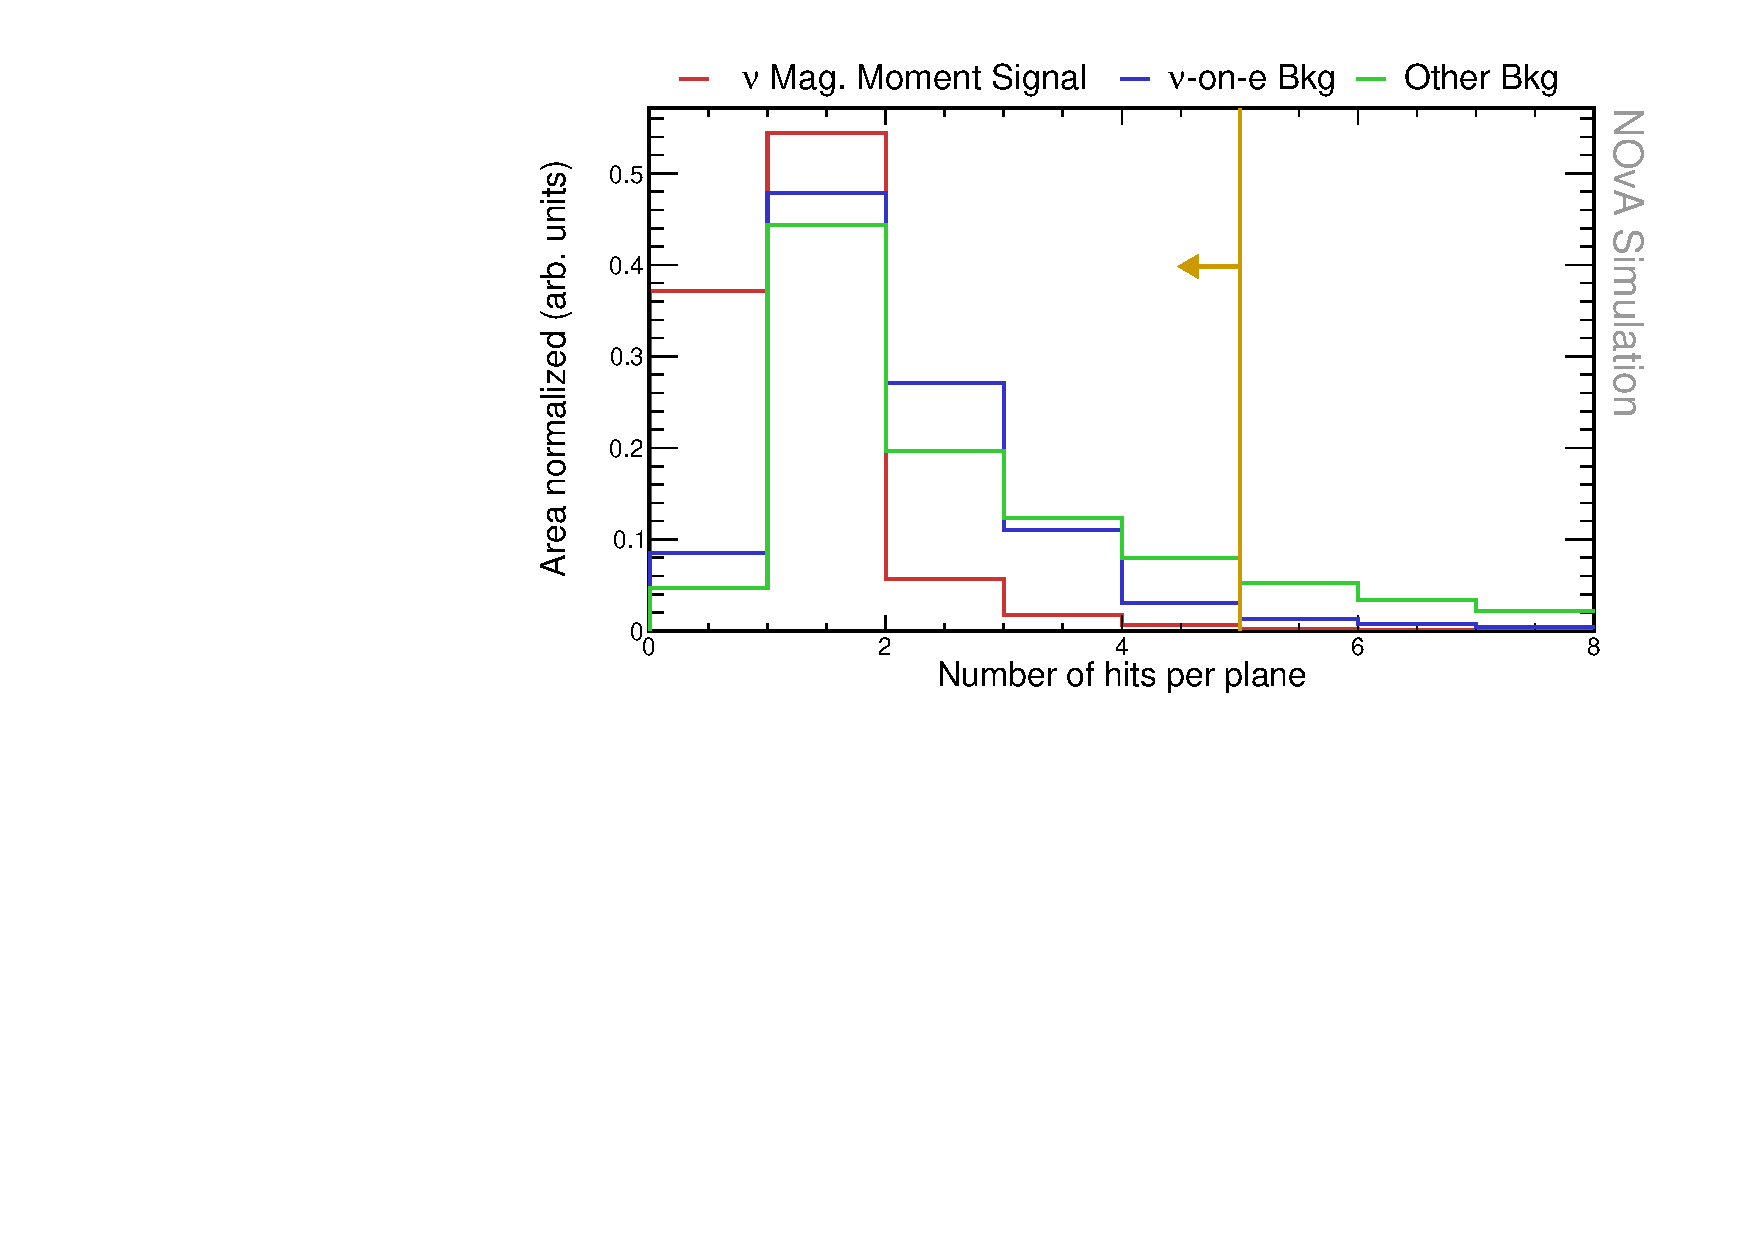
\includegraphics[width=.9\textwidth]{Plots/NuMMEventSelection/N1Cut_NHitsPPlane.pdf}
\caption[Prong and hits reconstruction quality cuts]{Relative comparison of signal (red), \acrshort{nuone} background (blue), and other background (green) events in the number of prongs (top) and the number of hits per plane (bottom) distributions. Events in both plots are required to have a valid reconstructed vertex and in the bottom plot also at least one reconstructed prong. Yellow lines indicate the cut values for the shown variables, with arrows pointing towards the preserved events. All histograms are area-normalised.}
\label{fig:NuMMCutsRecoQuality}
\end{figure}

%%% Low CalE
\note{Already applying the cut here to help reduce the events for TMVA. This cut is based purely on reco quality (we don't trust events below 0.5GeV, especially not for the CVN nuone ID variables}

\todo{discuss the energy cut, should this be removed? What is the effect on the event count? Why was this included in the first place (the identifiers are not as strong for lower energies - is this true though? - also there are further unexplored backgrounds that would need to be further studied and explore. Maybe depends on where would we move the cut...)}

The reconstructed calorimetric energy of the primary shower is required to be $E_{cal} > \unit[0.5]{GeV}$ as shown in Fig.~\ref{fig:NuMMCutsLowCalE}. This is to remove region in the parameter space with large backgrounds. However, due to the nature of the neutrino magnetic moment signal, this cut also removes a majority of our signal events (exactly how much?). 

This is due to a presence of large background that has not been studied very well. No \gls{NOvA} analysis really uses events with such low energies. However, after further studies and validation, it is likely that these cut can be pushed to lower electron recoil energy, especially by using better event identifiers to remove the large background there. 

NOvA is not super well suited for a low energy detection and there are troubles identifying very low energetic event. Majority of the analyses in NOvA only use events with energies above $\unit[0.5]{GeV}$.
nueCCXSec only uses events above 1 GeV. The  numuCCpi0 XSec ana had a low E cutoff at 0.1GeV

\note{How does the energy resolution and bias come into play here? 0.5GeV for us is not the same as for the 3fl or for some other ND analyses. This needs to be properly investigated in the future}

Maybe also say that Test Beam will be crucial in improving the vertex and energy resolution within NOvA, including electrons.

\begin{figure}[hbtp]
\centering
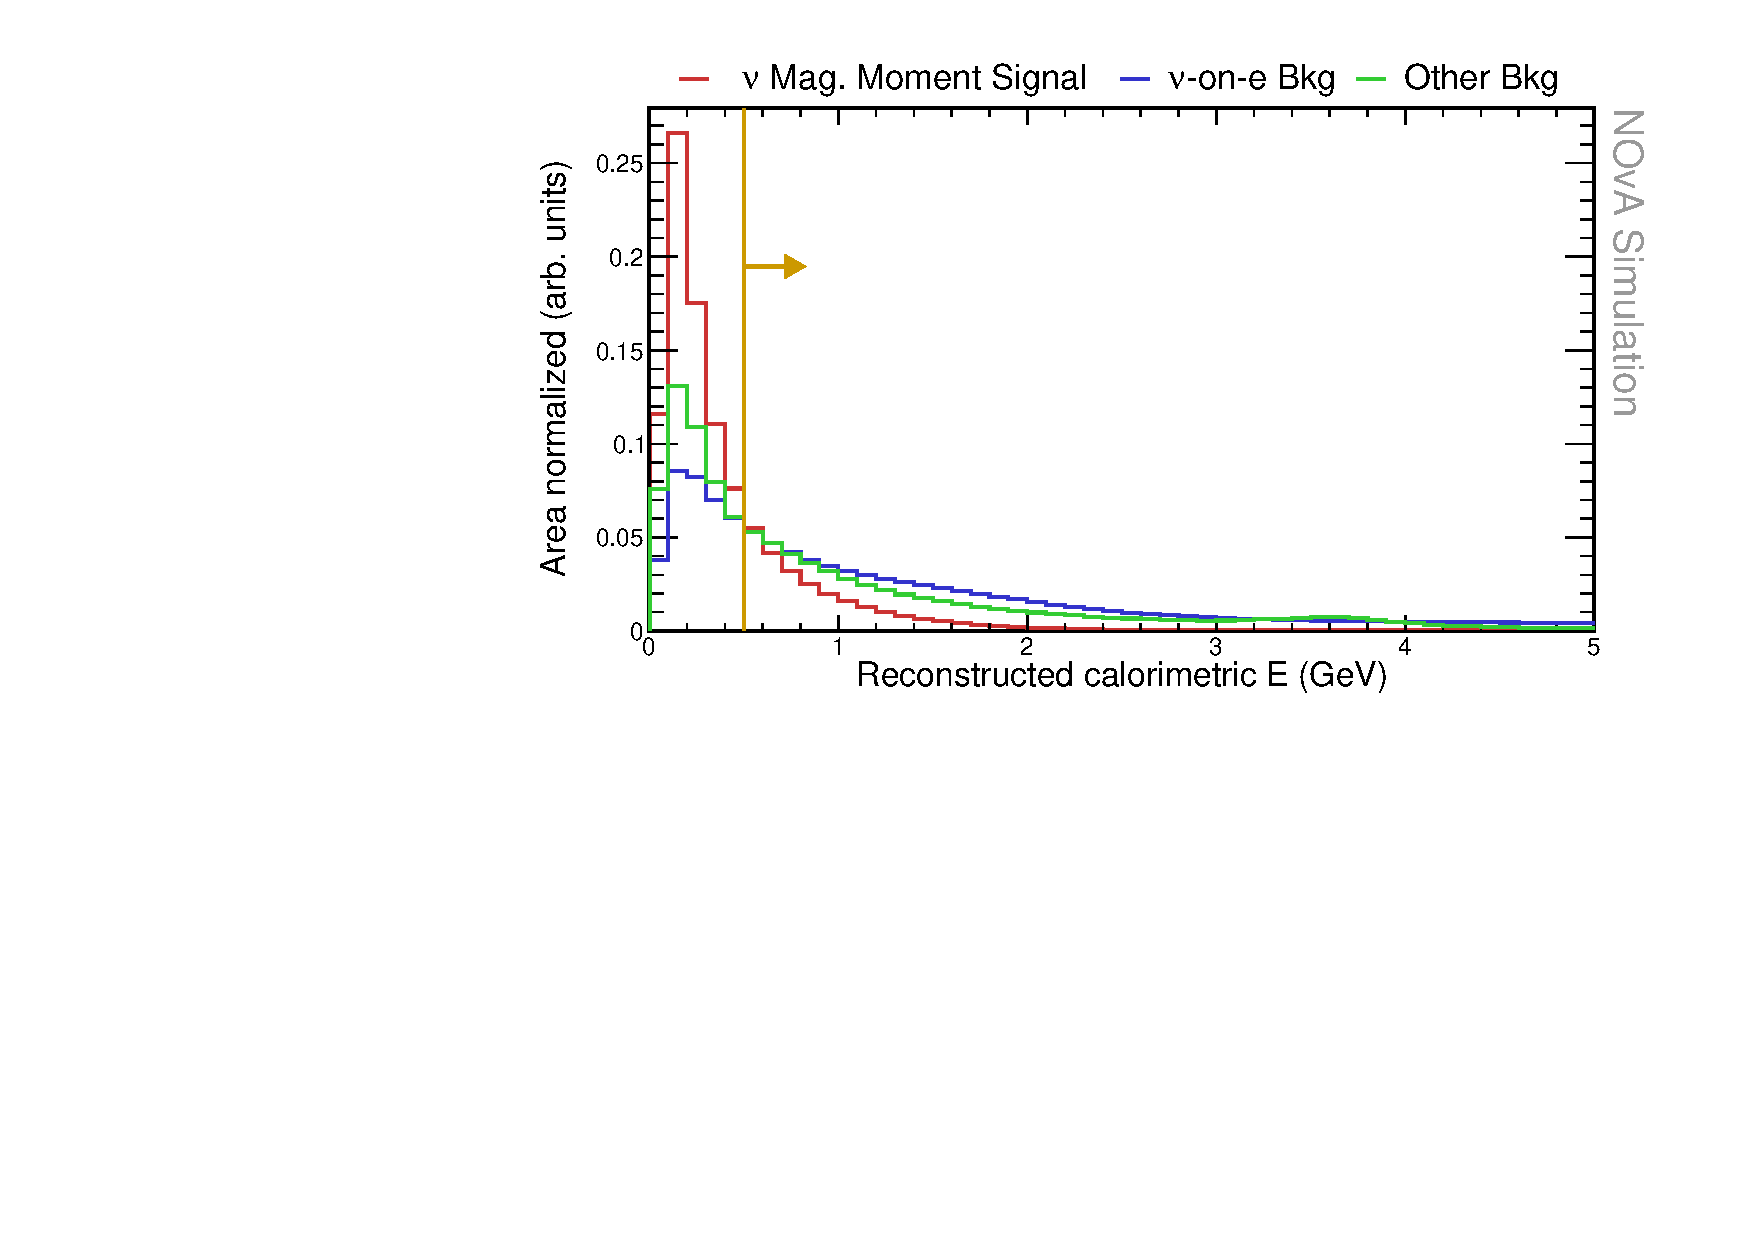
\includegraphics[width=.9\textwidth]{Plots/NuMMEventSelection/N1Cut_calELow.pdf}
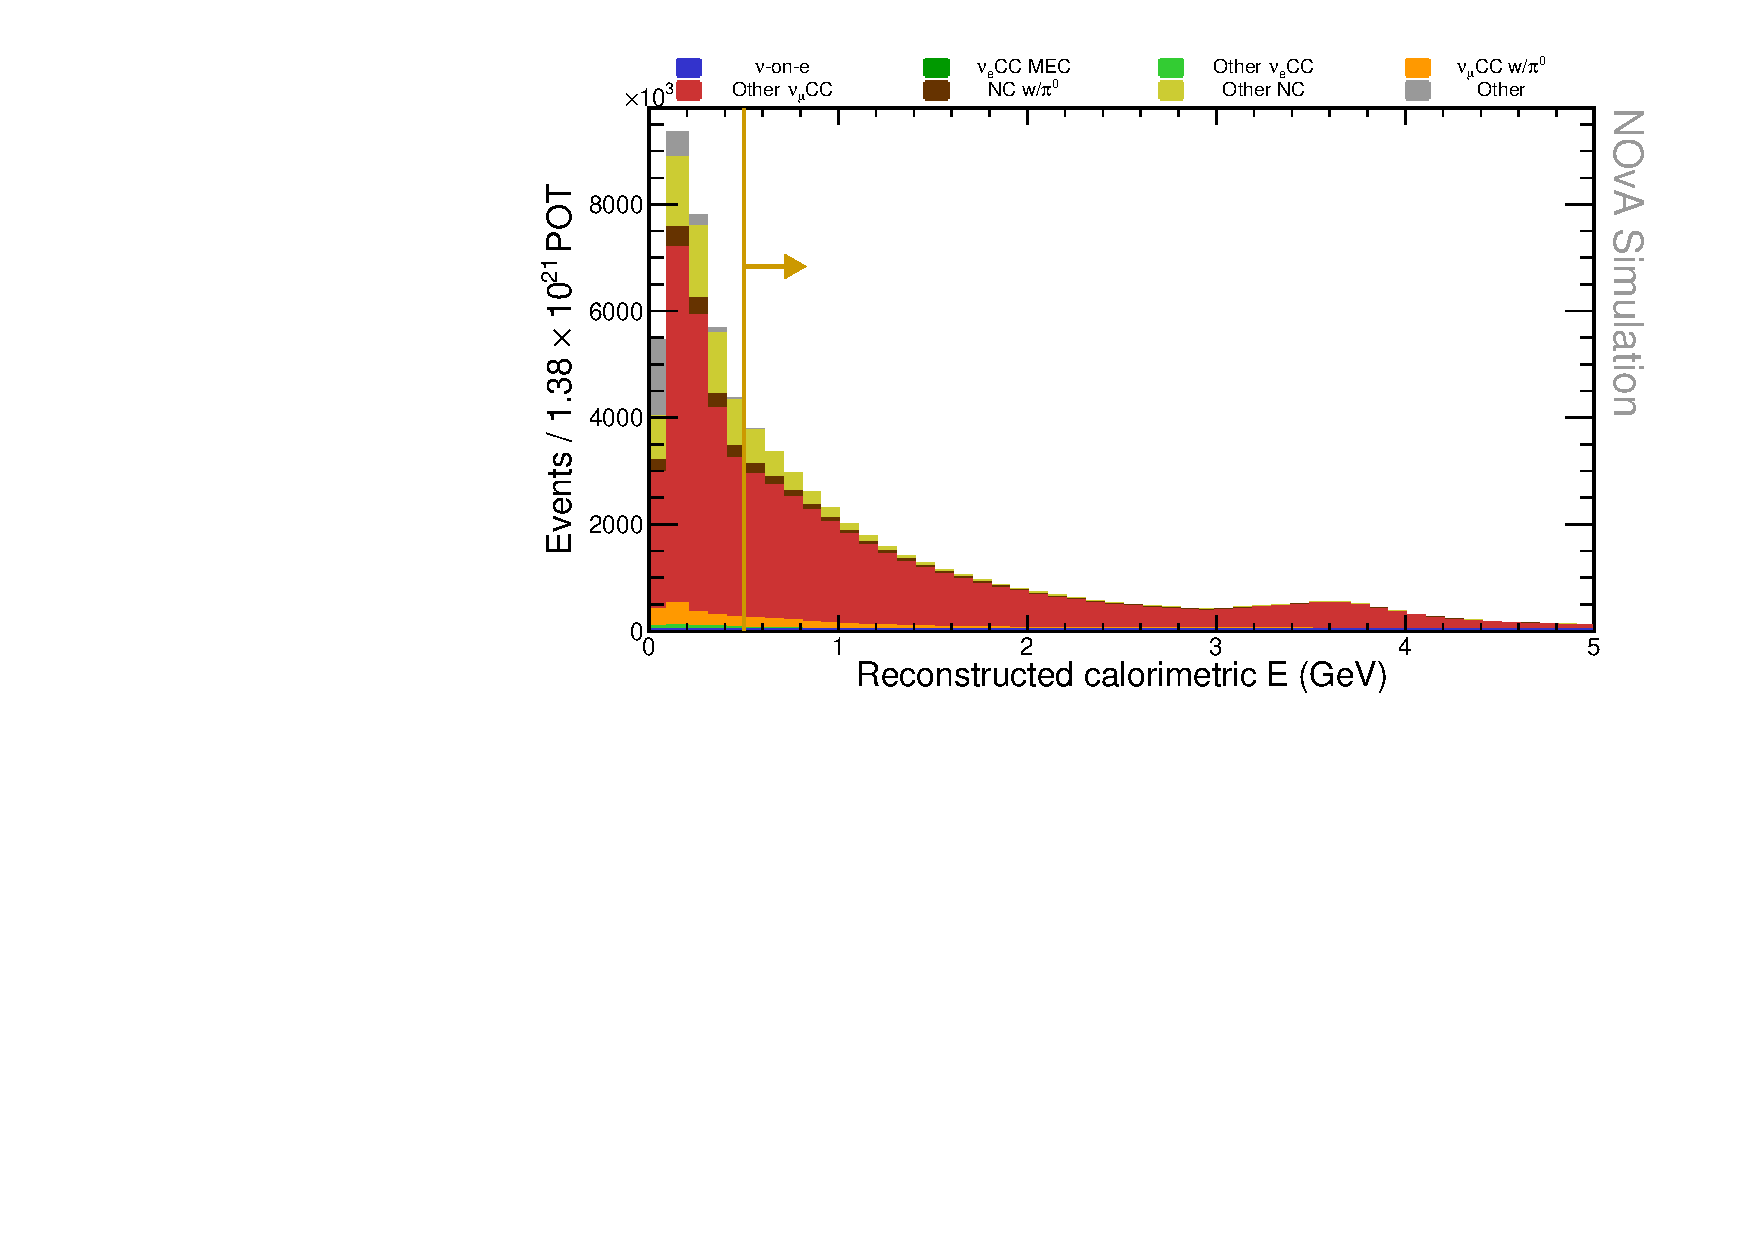
\includegraphics[width=.9\textwidth]{Plots/NuMMEventSelection/N1Cut_calELow_BkgDecomp.pdf}
\caption[Low calorimetric energy cut for reconstruction quality]{Top: Relative comparison of signal (red), \acrshort{nuone} background (blue), and other background (green) events in the reconstructed calorimetric energy distribution. All histograms are area-normalised. Bottom: Decomposition of background into various sub-samples, normalised to the data \acrshort{POT} exposure. Events in both plots are required to have a valid reconstructed vertex, at least one reconstructed prong and at most $5$ hits per plane. Yellow lines indicate the cut value for the reconstructed calorimetric energy, with arrows pointing towards the preserved events.}
\label{fig:NuMMCutsLowCalE}
\end{figure}

\begin{table}[!hb]
\centering
\caption[Event selection cutflow table for the reconstruction quality cuts]{Event selection cutflow table for the reconstruction quality cuts showing the number of events and the relative efficiency of each cut for each signal sample. The relative efficiency is calculated as number of events remaining after applying the corresponding cut divided by number of event for all the previous cuts. All the cuts are listed in sequence as they are applied.}
\begin{tabular}{|l|cc|cc|cc|}\hline
\multicolumn{1}{|c|}{} & \multicolumn{2}{c|}{\textbf{Signal}} & \multicolumn{2}{c|}{\textbf{$\nu$-on-e bkg}} & \multicolumn{2}{c|}{\textbf{Other bkg}} \\
\multicolumn{1}{|c|}{\multirow{-2}{*}{\textbf{Selection}}} & \textbf{$N_{evt}$} & \textbf{$\epsilon_{rel}\left(\%\right)$} & \textbf{$N_{evt}$} & \textbf{$\epsilon_{rel}\left(\%\right)$}  & \textbf{$N_{evt}$} & \textbf{$\epsilon_{rel}\left(\%\right)$}\\\hline
\textbf{No Cut} & 269.77 & 100 & 3.43$\times 10^3$ & 100 & 2.96$\times 10^8$ & 100\\
\textbf{Valid Vtx} & 180.58 & 66.94 & 3.33$\times 10^3$ & 96.94 & 2.34$\times 10^8$ & 79.10\\
\textbf{N$^o$ Prongs} & 174.69 & 96.74 & 3.23$\times 10^3$ & 96.99 & 8.66$\times 10^7$ & 37.00\\
\textbf{Hits / Plane} & 174.36 & 99.81 & 3.22$\times 10^3$ & 93.83 & 7.32$\times 10^7$ & 84.55\\
\textbf{Low $E_{Shower}$} & 48.75 & 27.96 & 2.71$\times 10^3$ & 84.10 & 4.06$\times 10^7$ & 55.52\\\hline
\end{tabular}
\label{tab:CutflowTableBasicRecoQC}
\end{table}

\subsection{Basic Event Selection}

Basic event selection cuts aim to remove obvious background events without affecting the signal too much. The criterion for these cuts will be that each of them has to limit the signal efficiency by approximately $\unit[0.25]{\%}$. This means that in total the pre-selection cuts will lower the signal efficiency by only approximately $\unit[1]{\%}$. We are using the same variables for these cuts as were used in the event selection for the $\nu_e$ appearance \gls{ND} constraint for the three flavour neutrino oscillation measurements \cite{NOvAResults2021.pdf}. Additionally, we are also using a cut on the product of the reconstructed calorimetric energy and the square of the reconstructed angle between the recoil electron and the neutrino beam direction. The electron is assumed to be the most energetic reconstructed showers. The reconstructed showers are ordered based on their deposited energies, therefore the first reconstructed prong is assumed to be the most energetic. In case of the \gls{nuone} events, this should be the electron.

They also remove the obvious $\nu_\mu$CC interactions by requiring that the summed number of cells for all prongs in the slice is $<200$ and the length of the longest prong is $<540\ \unit{cm}$. Relative comparison of signal, \gls{nuone} background, and other background distributions for the pre-selection variables is shown on Fig.~\ref{fig:PreSelectionCuts}.

Additionally, as discussed in Sec.~\ref{sec:MeasuringNuMM}, from theory we know what the true recoil electron for the \gls{nuone} interaction is supposed to be limited by $E\theta^2<2m_e$. Due to reconstruction deficiencies, the reconstructed $E\theta^2$ will not have such a strict cut-off for \gls{nuone} events, this variable can however be used to distinguish them from the $\nu_e$\gls{CC} events, for which the electron has a much more isotropic distribution.

On top of that, we are also placing a loose cut on the maximum calorimetric energy, as the signal is limited to low energies, as can be seen in Fig.~\ref{fig:NuMMCutsETh2CalEHighLoose}.

Some of the signal events can be reconstructed with the opposite direction than the beam. These events might still be useful though and we want to keep them. For that reason, we are calculating the angle between the outgoing electron and the neutrino beam direction as $\textsf{acos}\left(\textsf{abs}\left(\cos\theta\right)\right)$, which gives the same value whether the shower is reconstructed forward or backwards.

\begin{figure}[hbtp]
\centering
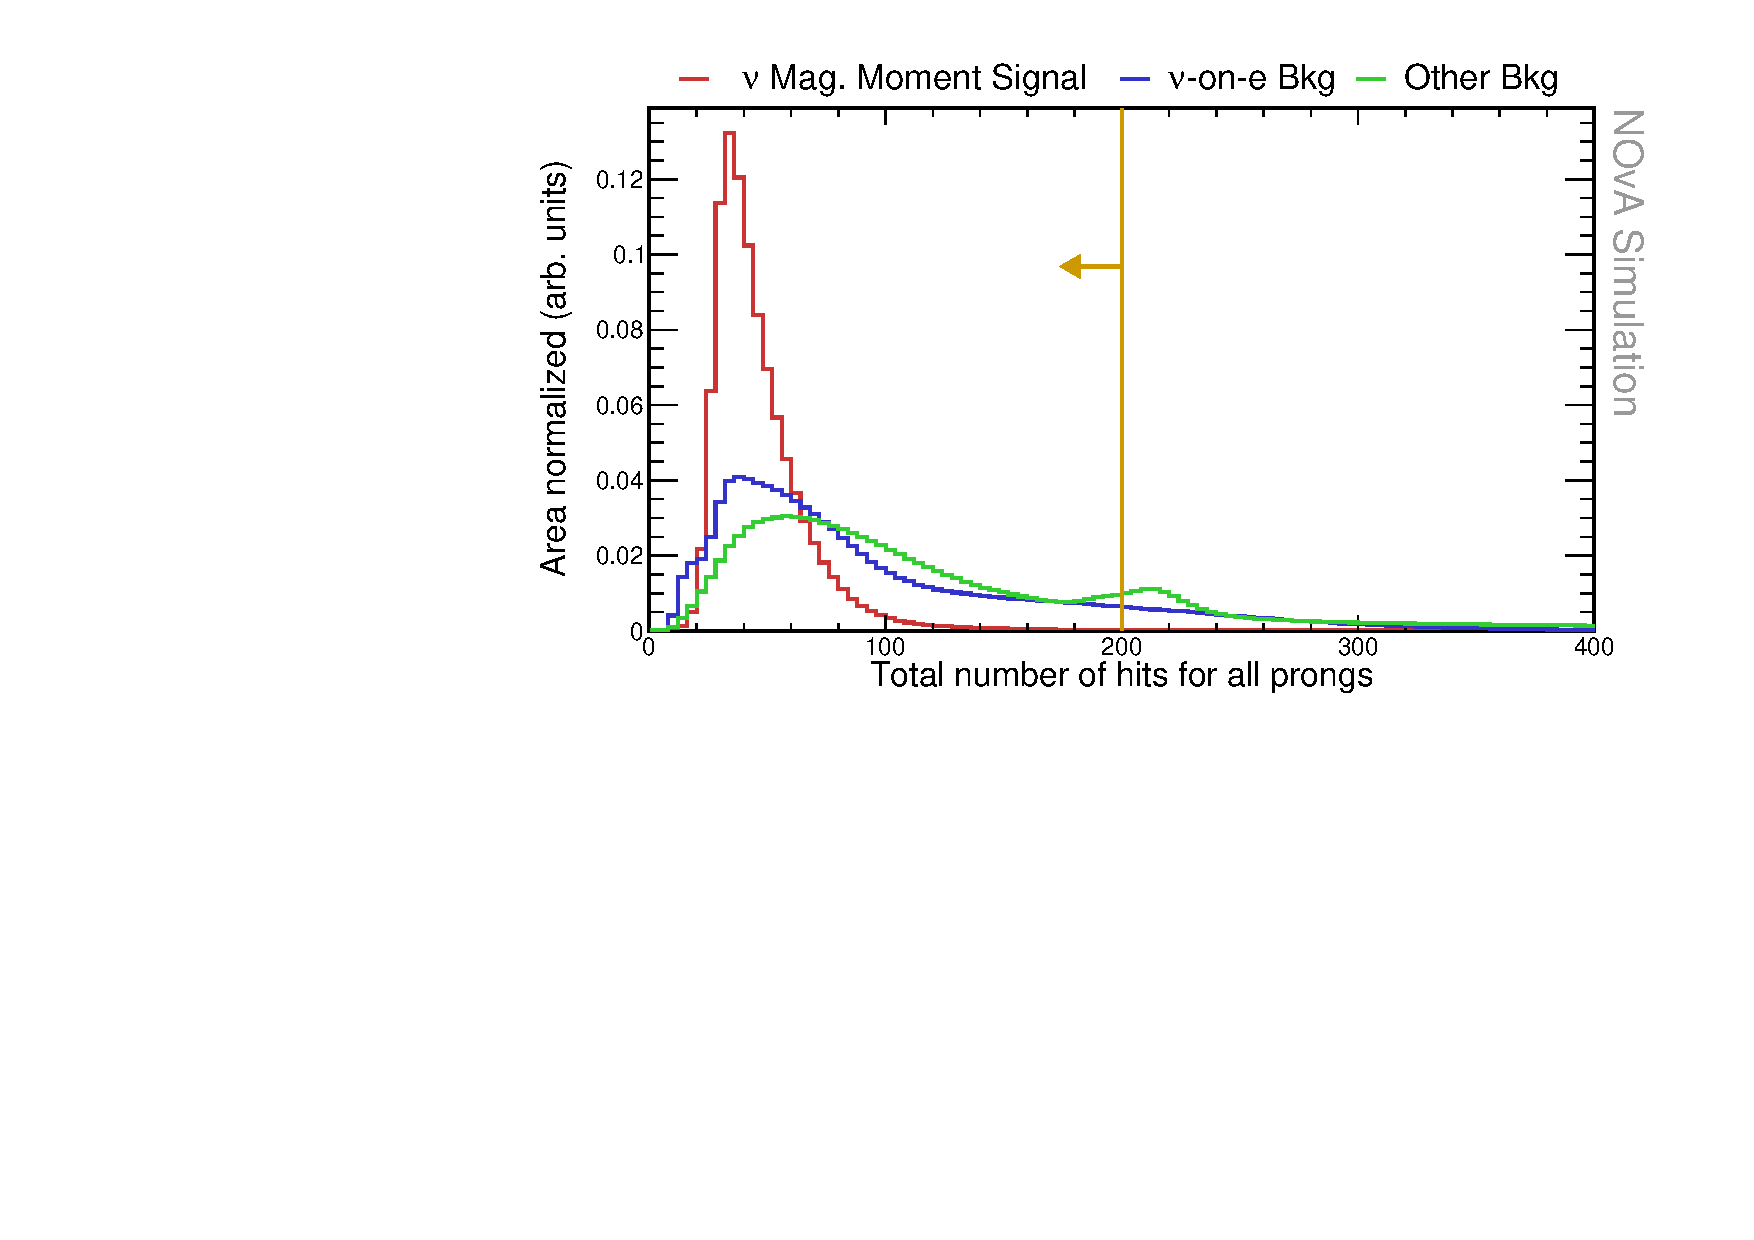
\includegraphics[width=.9\textwidth]{Plots/NuMMEventSelection/N1Cut_NHits.pdf}
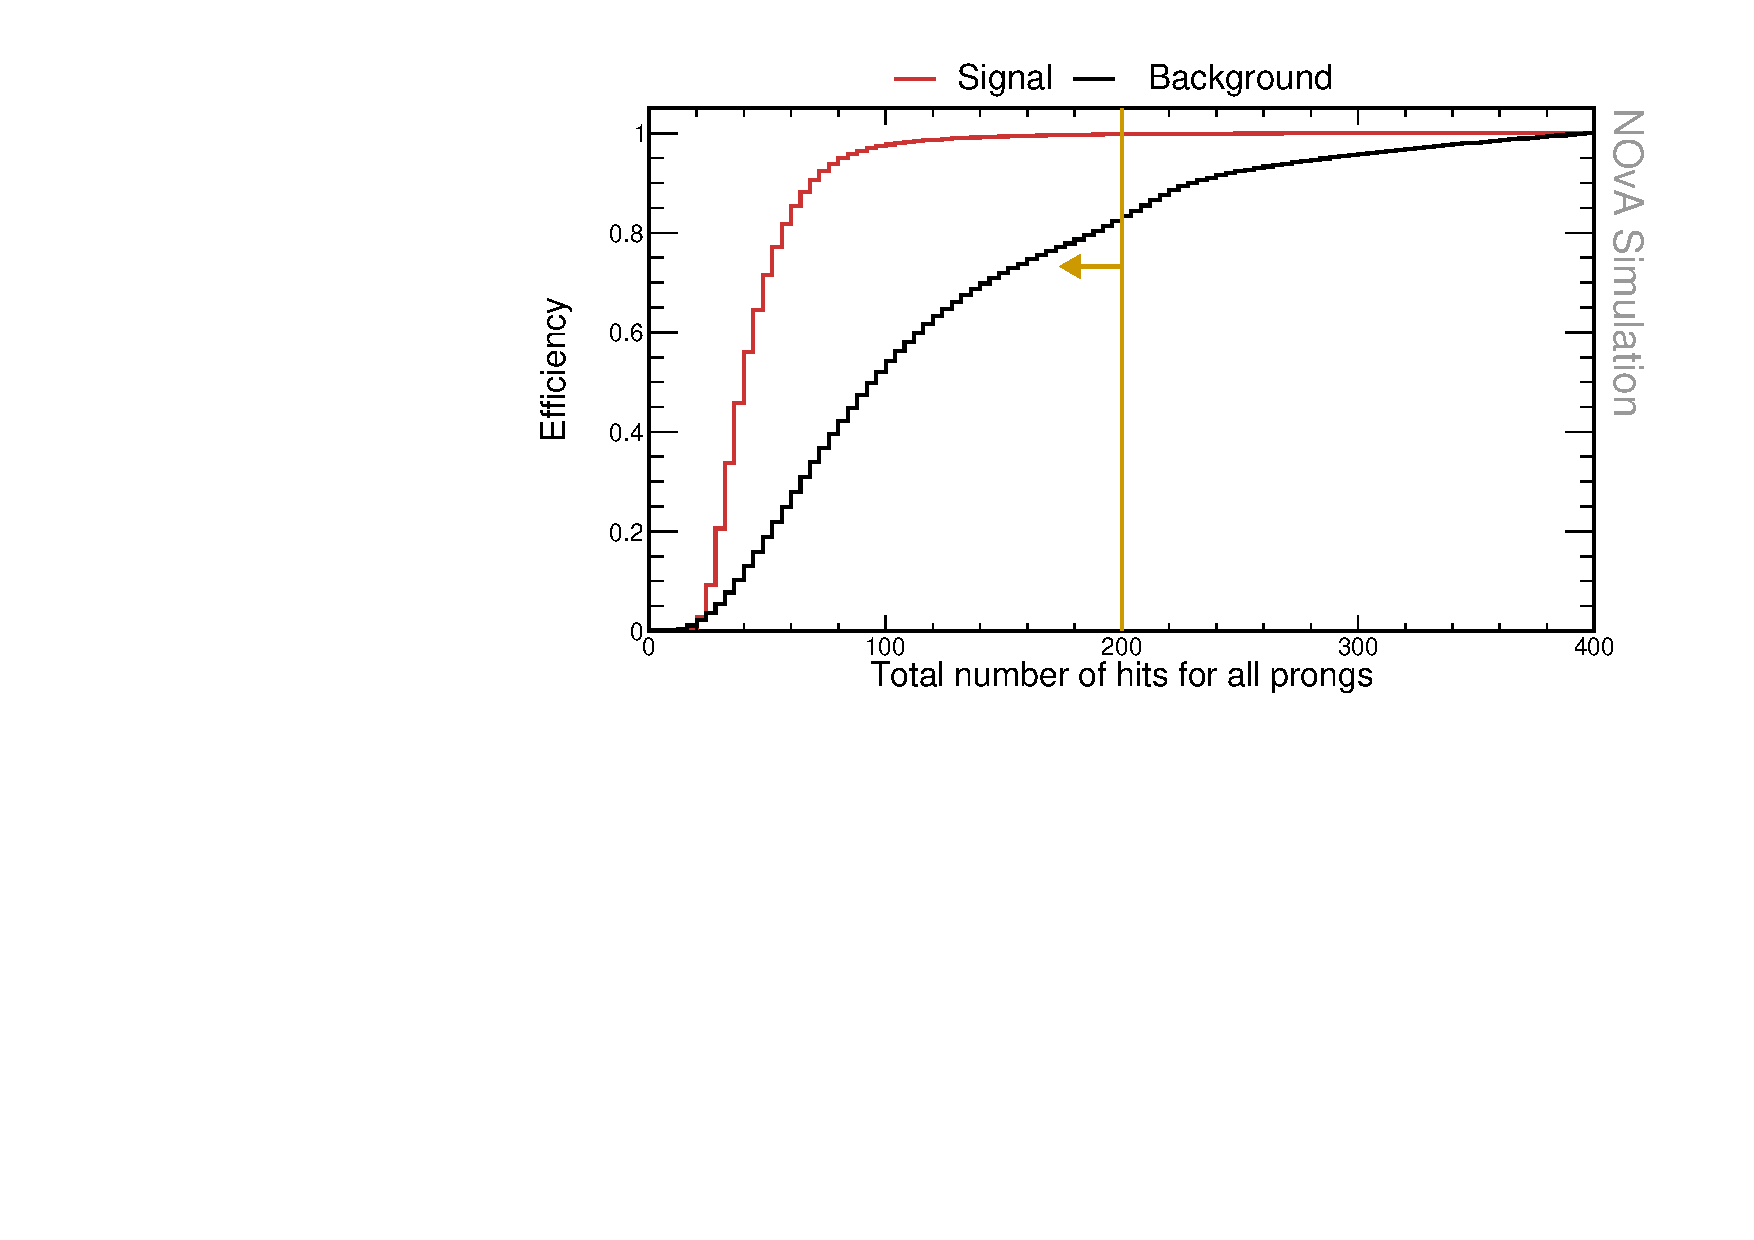
\includegraphics[width=.9\textwidth]{Plots/NuMMEventSelection/NuMM_N1Cut_NHitsleft_Eff.pdf}
\caption[Number of hits cut for basic event selection]{Top: Relative comparison of signal (red), \acrshort{nuone} background (blue), and other background (green) events in the distribution of total number of hits from all reconstructed prongs in the slice. All histograms are area-normalised. Bottom: Cumulative signal (red) and background (black) efficiency calculated as number of signal/background events left of the bin divided by the total number of signal/background events. Yellow lines indicate the cut value for the maximum number of hits, with arrows pointing towards the preserved events. The reconstruction quality cuts were applied before making these plots.}
\label{fig:NuMMCutsNHits}
\end{figure}

\begin{figure}[hbtp]
\centering
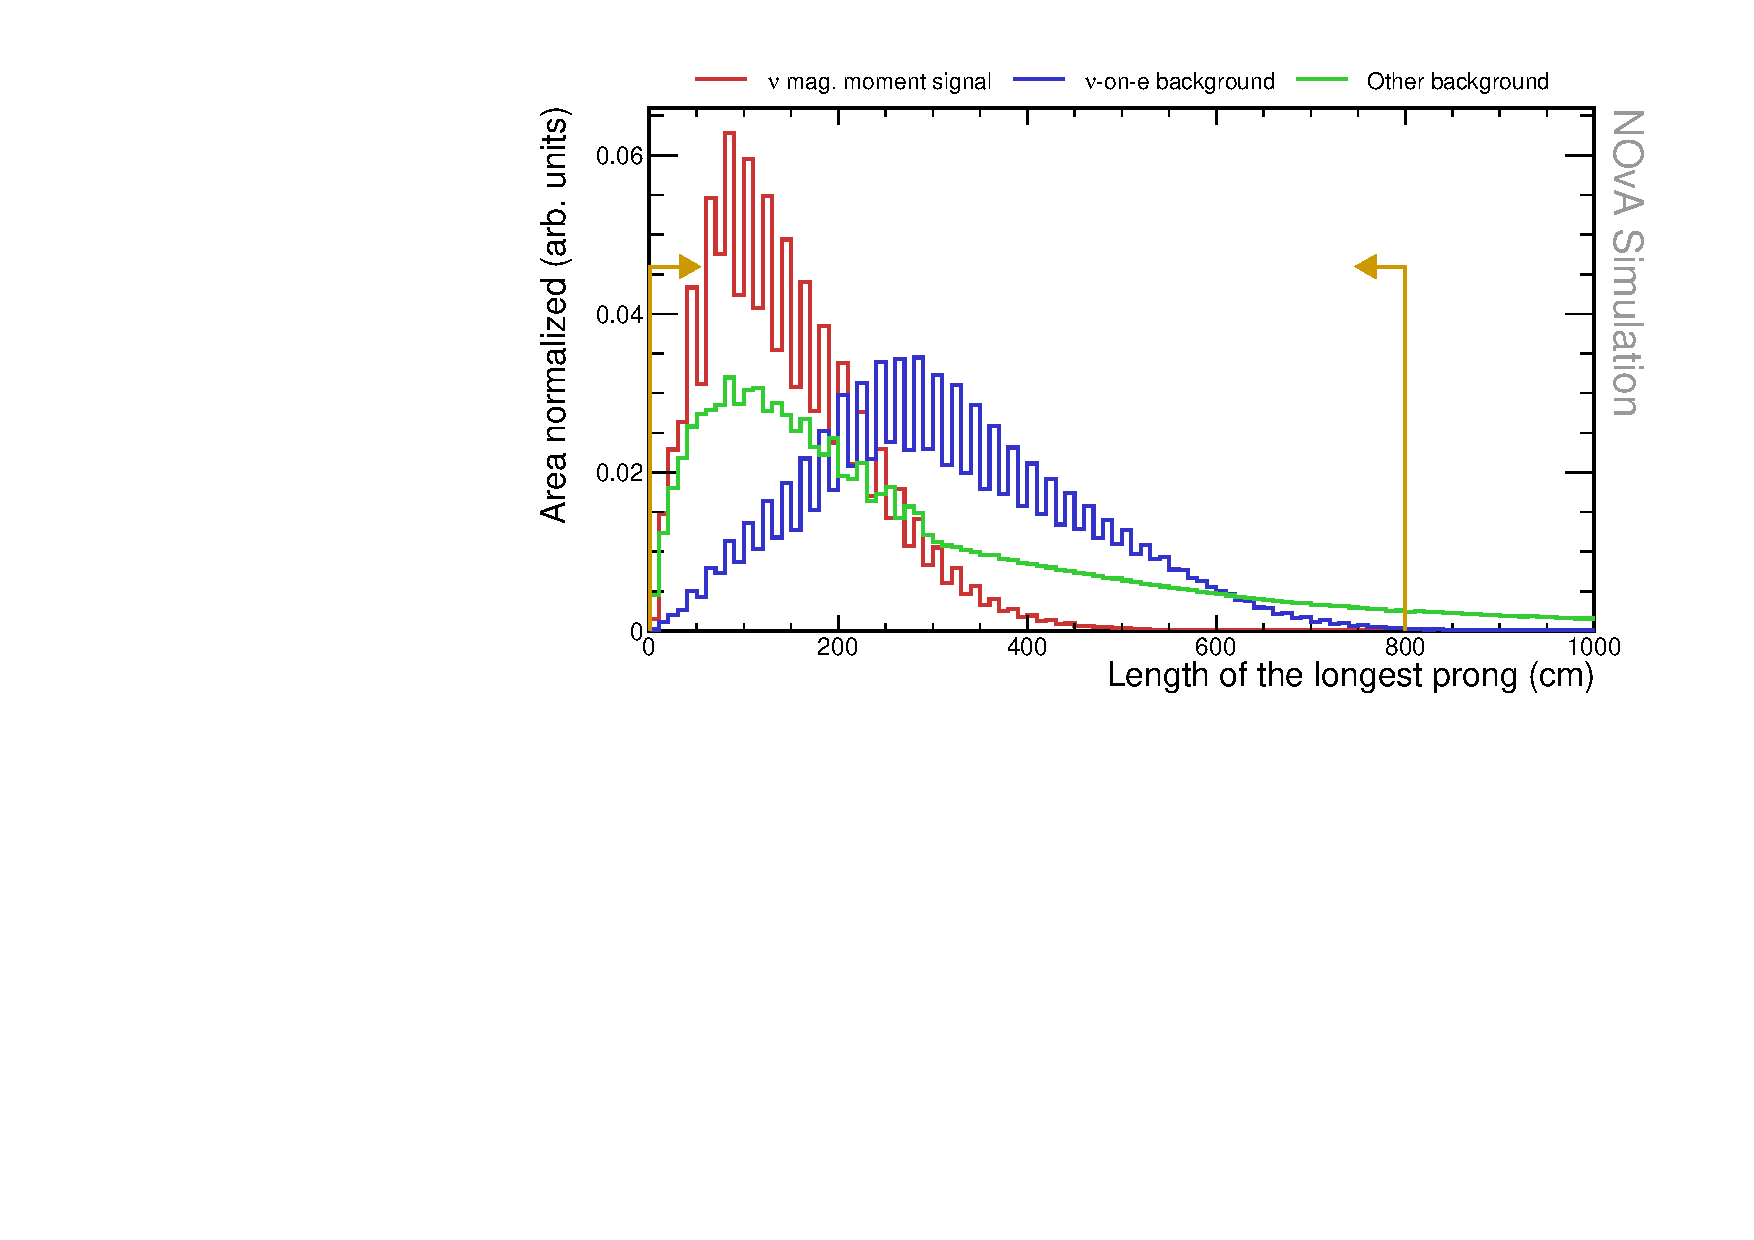
\includegraphics[width=.9\textwidth]{Plots/NuMMEventSelection/N1Cut_longestProng.pdf}
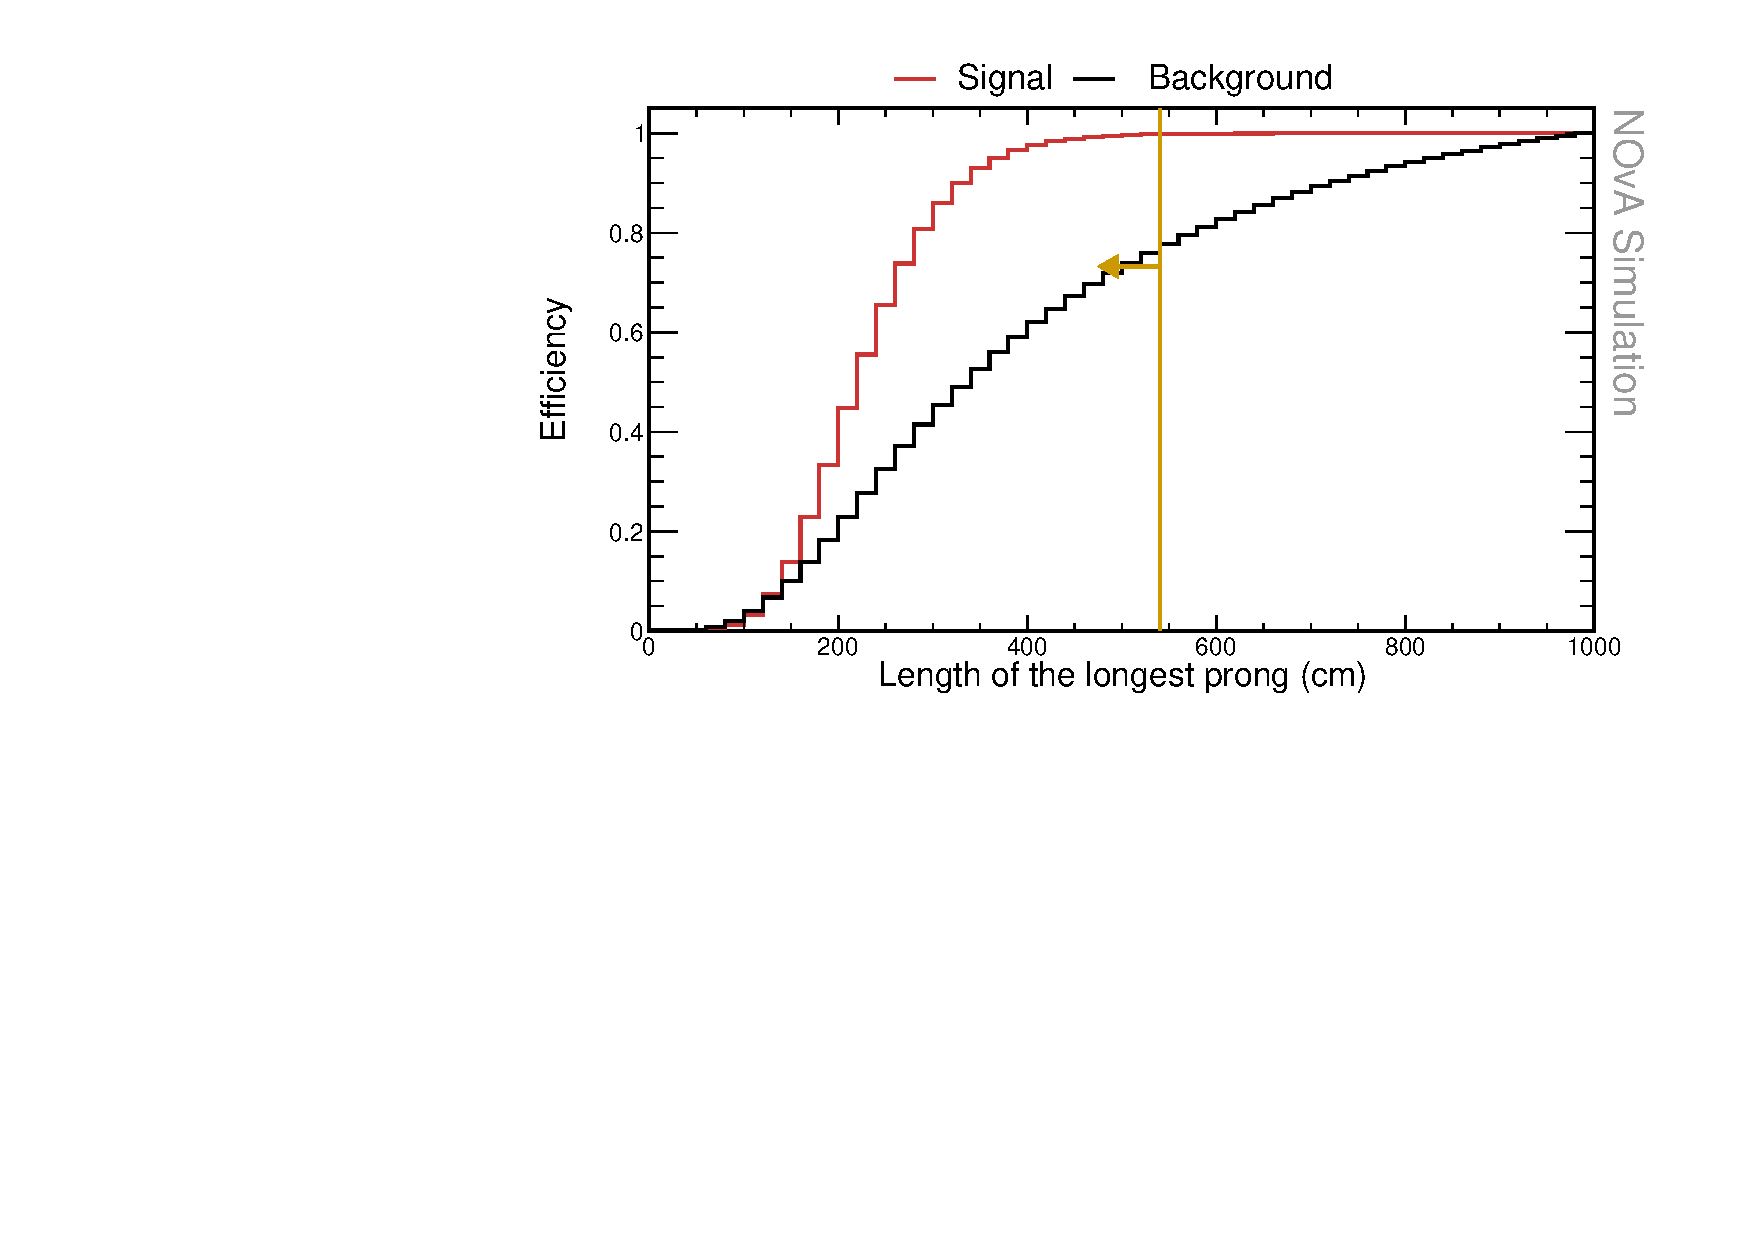
\includegraphics[width=.9\textwidth]{Plots/NuMMEventSelection/NuMM_N1Cut_longestProngleft_Eff.pdf}
\caption[Length of the longest prong cut for basic event selection]{Top: Relative comparison of signal (red), \acrshort{nuone} background (blue), and other background (green) events in the distribution of the length of the longest reconstructed prong in slice. All histograms are area-normalised. Bottom: Cumulative signal (red) and background (black) efficiency calculated as number of signal/background events left of the bin divided by the total number of signal/background events. Yellow lines indicate the cut value for the maximum length of the longest prong, with arrows pointing towards the preserved events. The reconstruction quality cuts and the number of hits cut were applied before making these plots.}
\label{fig:NuMMCutsLongestProng}
\end{figure}

\begin{figure}[hbtp]
\centering
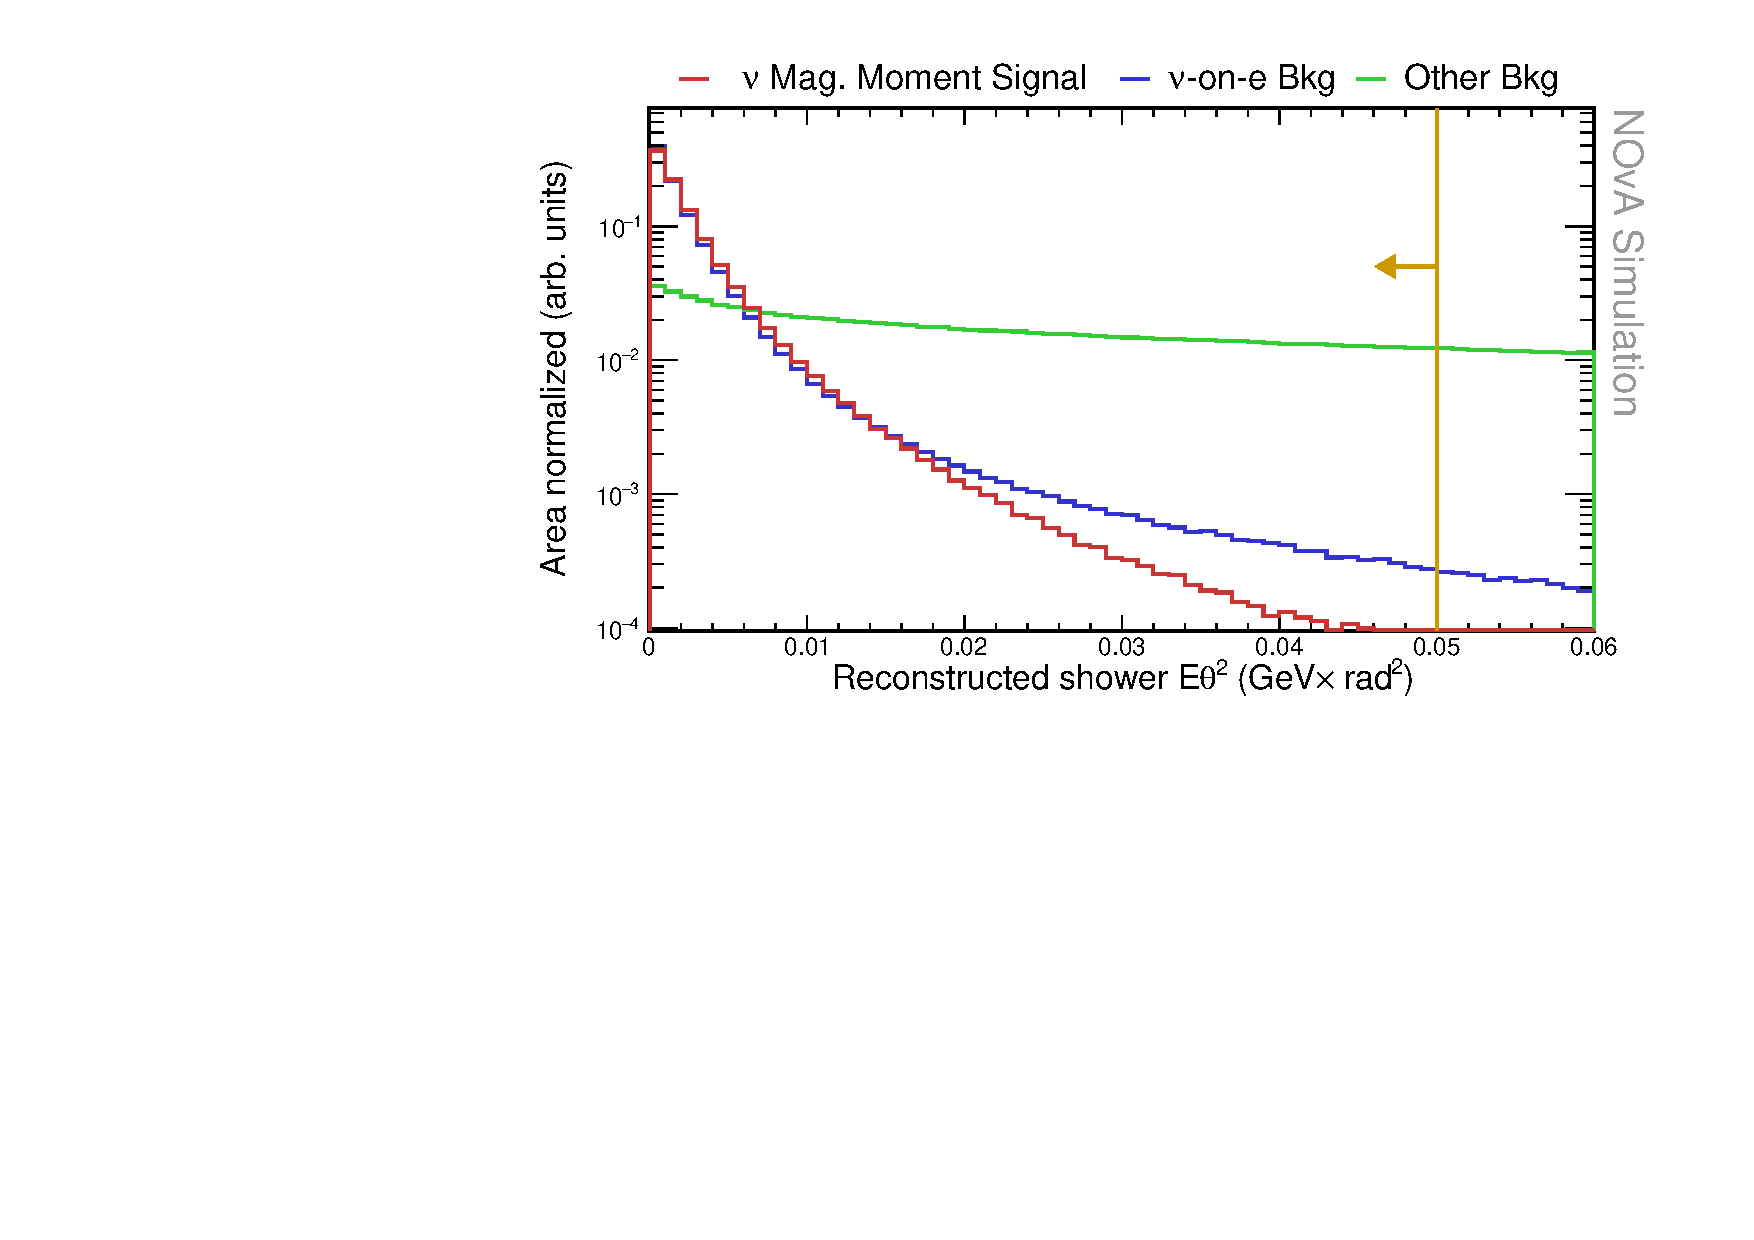
\includegraphics[width=.9\textwidth]{Plots/NuMMEventSelection/LogY_N1Cut_eth2Loose.pdf}
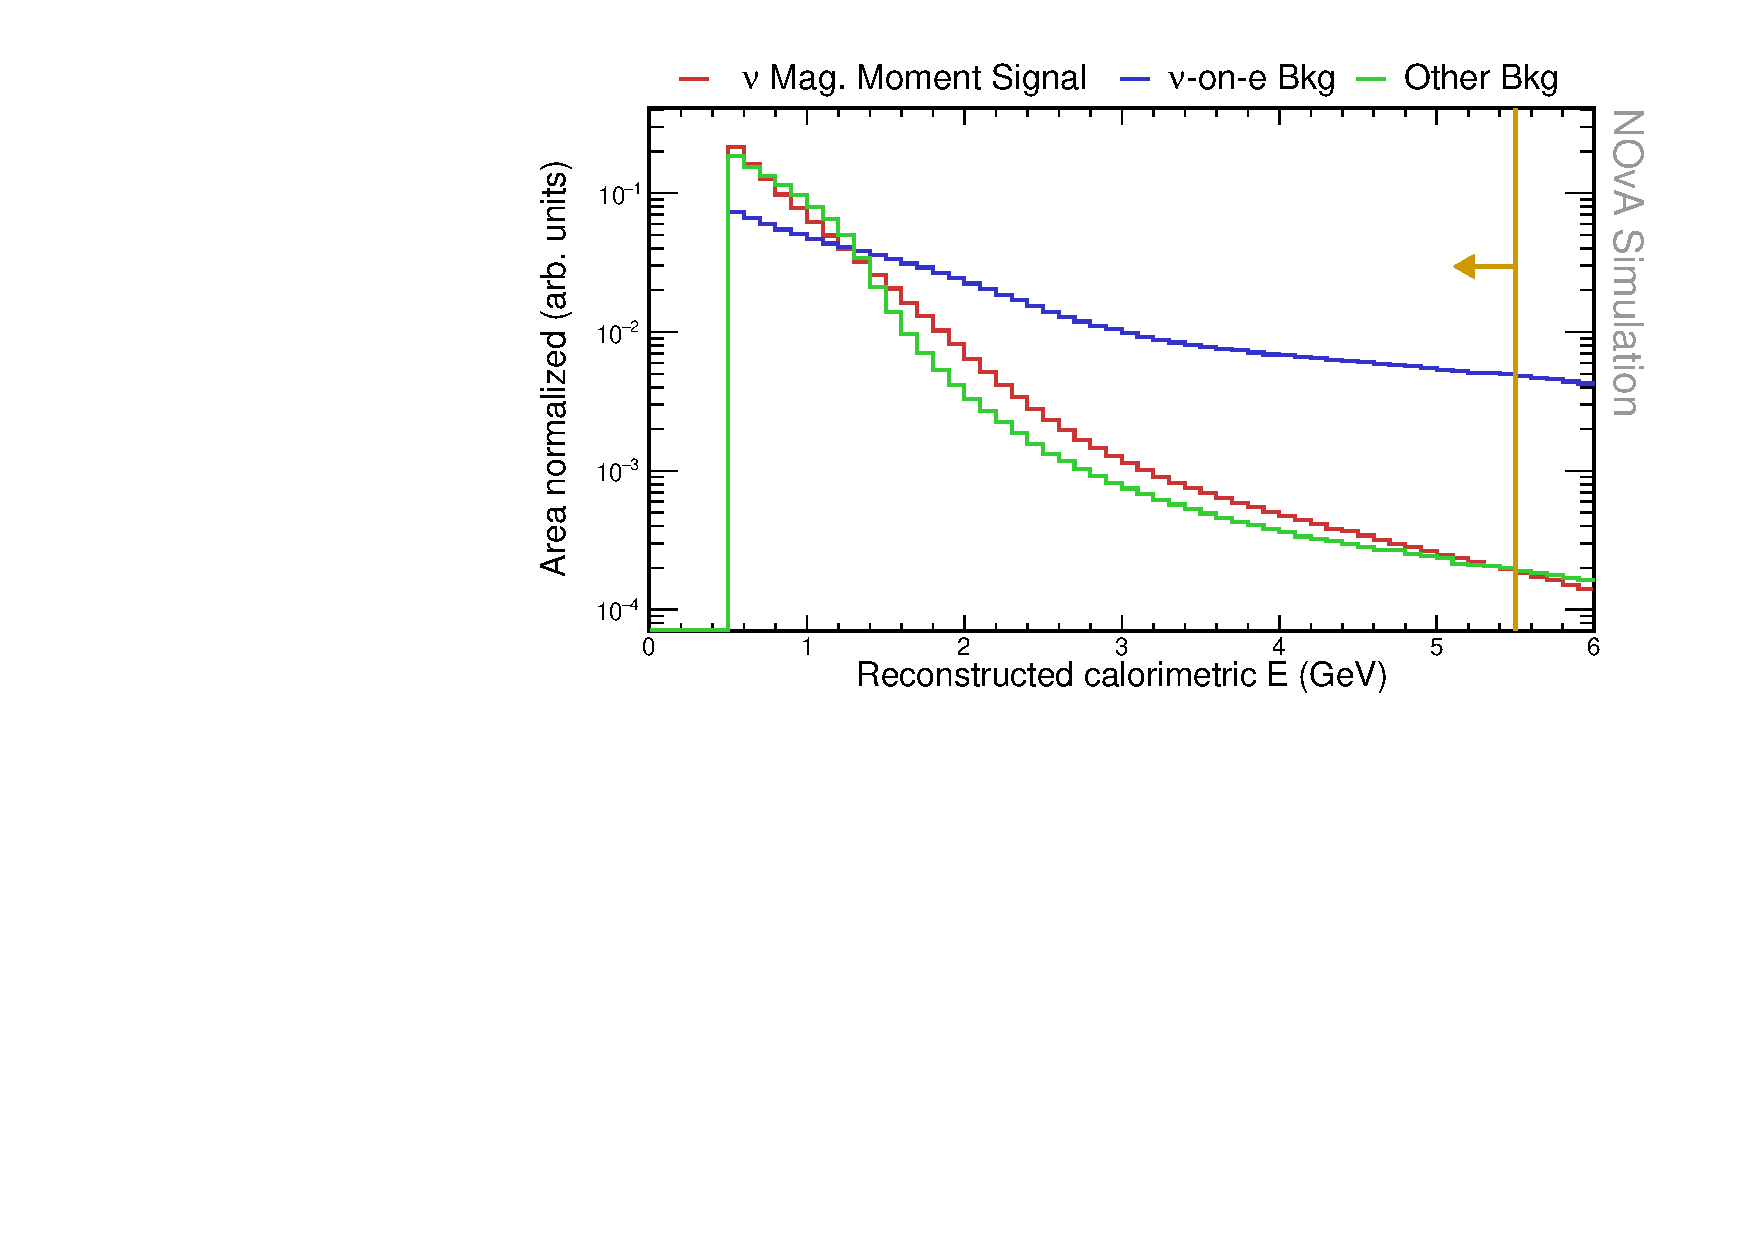
\includegraphics[width=.9\textwidth]{Plots/NuMMEventSelection/LogY_N1Cut_calEHighLoose.pdf}
\caption[$E\theta^2$ and high calorimetric energy cut for basic event selection]{Relative comparison of signal (red), \acrshort{nuone} background (blue), and other background (green) events in the distribution of the reconstructed energy of the leading shower multiplied by its angle from the incoming neutrino beam direction squared (top) and of the reconstructed energy of the leading shower (bottom). All histograms are area-normalised with logarithmic y axis. Yellow lines indicate the cut value for the corresponding variables, with arrows pointing towards the preserved events. The reconstruction quality cuts, the number of hits cut, and the length of the longest prong cuts were applied before making both of these plots, while the hits in the bottom plot are also required to pass the $E\theta^2$ cut.}
\label{fig:NuMMCutsETh2CalEHighLoose}
\end{figure}

%\todo{Add the DeCAF cuts description here - might describe them already when introducing the decaf samples, not sure yet}

\begin{table}[!hb]
\centering
\caption[Event selection cutflow table for the basic event selection]{Basic event selection cutflow table showing the number of events and the relative efficiency of each cut for each signal sample. The relative efficiency is calculated as number of events remaining after applying the corresponding cut divided by number of event for all the previous cuts. All the cuts are listed in sequence as they are applied. The top row corresponds to the sample after applying the reconstruction quality cuts.}
\begin{tabular}{|l|cc|cc|cc|}\hline
\multicolumn{1}{|c|}{} & \multicolumn{2}{c|}{\textbf{Signal}} & \multicolumn{2}{c|}{\textbf{$\nu$-on-e bkg}} & \multicolumn{2}{c|}{\textbf{Other bkg}} \\
\multicolumn{1}{|c|}{\multirow{-2}{*}{\textbf{Selection}}} & \textbf{$N_{evt}$} & \textbf{$\epsilon_{rel}\left(\%\right)$} & \textbf{$N_{evt}$} & \textbf{$\epsilon_{rel}\left(\%\right)$}  & \textbf{$N_{evt}$} & \textbf{$\epsilon_{rel}\left(\%\right)$}\\\hline
\textbf{Reco Quality} & 48.75 & 100 & 2.71$\times 10^3$ & 100 & 4.06$\times 10^7$ & 100\\
\textbf{N$^o$ Hits Loose} & 48.64 & 99.78 & 2.32$\times 10^3$ & 85.63 & 3.08$\times 10^7$ & 75.67\\
\textbf{Prong Length} & 48.52 & 99.75 & 2.26$\times 10^3$ & 97.39 & 2.17$\times 10^7$ & 70.66\\
\textbf{$E\theta^2$ Loose} & 48.39 & 99.73 & 2.25$\times 10^3$ & 99.71 & 6.00$\times 10^6$ & 27.62\\
\textbf{High $E_{Shower}$ Loose} & 48.27 & 99.76 & 2.03$\times 10^3$ & 90.04 & 5.98$\times 10^6$ & 99.67\\\hline
\end{tabular}
\label{tab:CutflowTableBasicSelection}
\end{table}

\subsection{Fiducial and containment cuts}

[nueXSec ana, docdb:37668] For both the X and Y vertices the distributions are asymmetric when comparing across the origin, in terms of vertex position. This is primarily due to particles coming from the +y and -x from events in the rock surrounding the detector. This corresponds to the direction of the NuMI target from the near detector. ...We require all activity from neutrino activity be deposited outside of the muon catcher.

\todo{Describe what does the fiducial cut do}
We require that the reconstructed vertex is contained within the following volume: $-175<\textsf{Vtx}_X<175,-175<\textsf{Vtx}_Y<175, 95<\textsf{Vtx}_Z<1095\ \unit{cm}$.

\begin{figure}[hbtp]
\centering
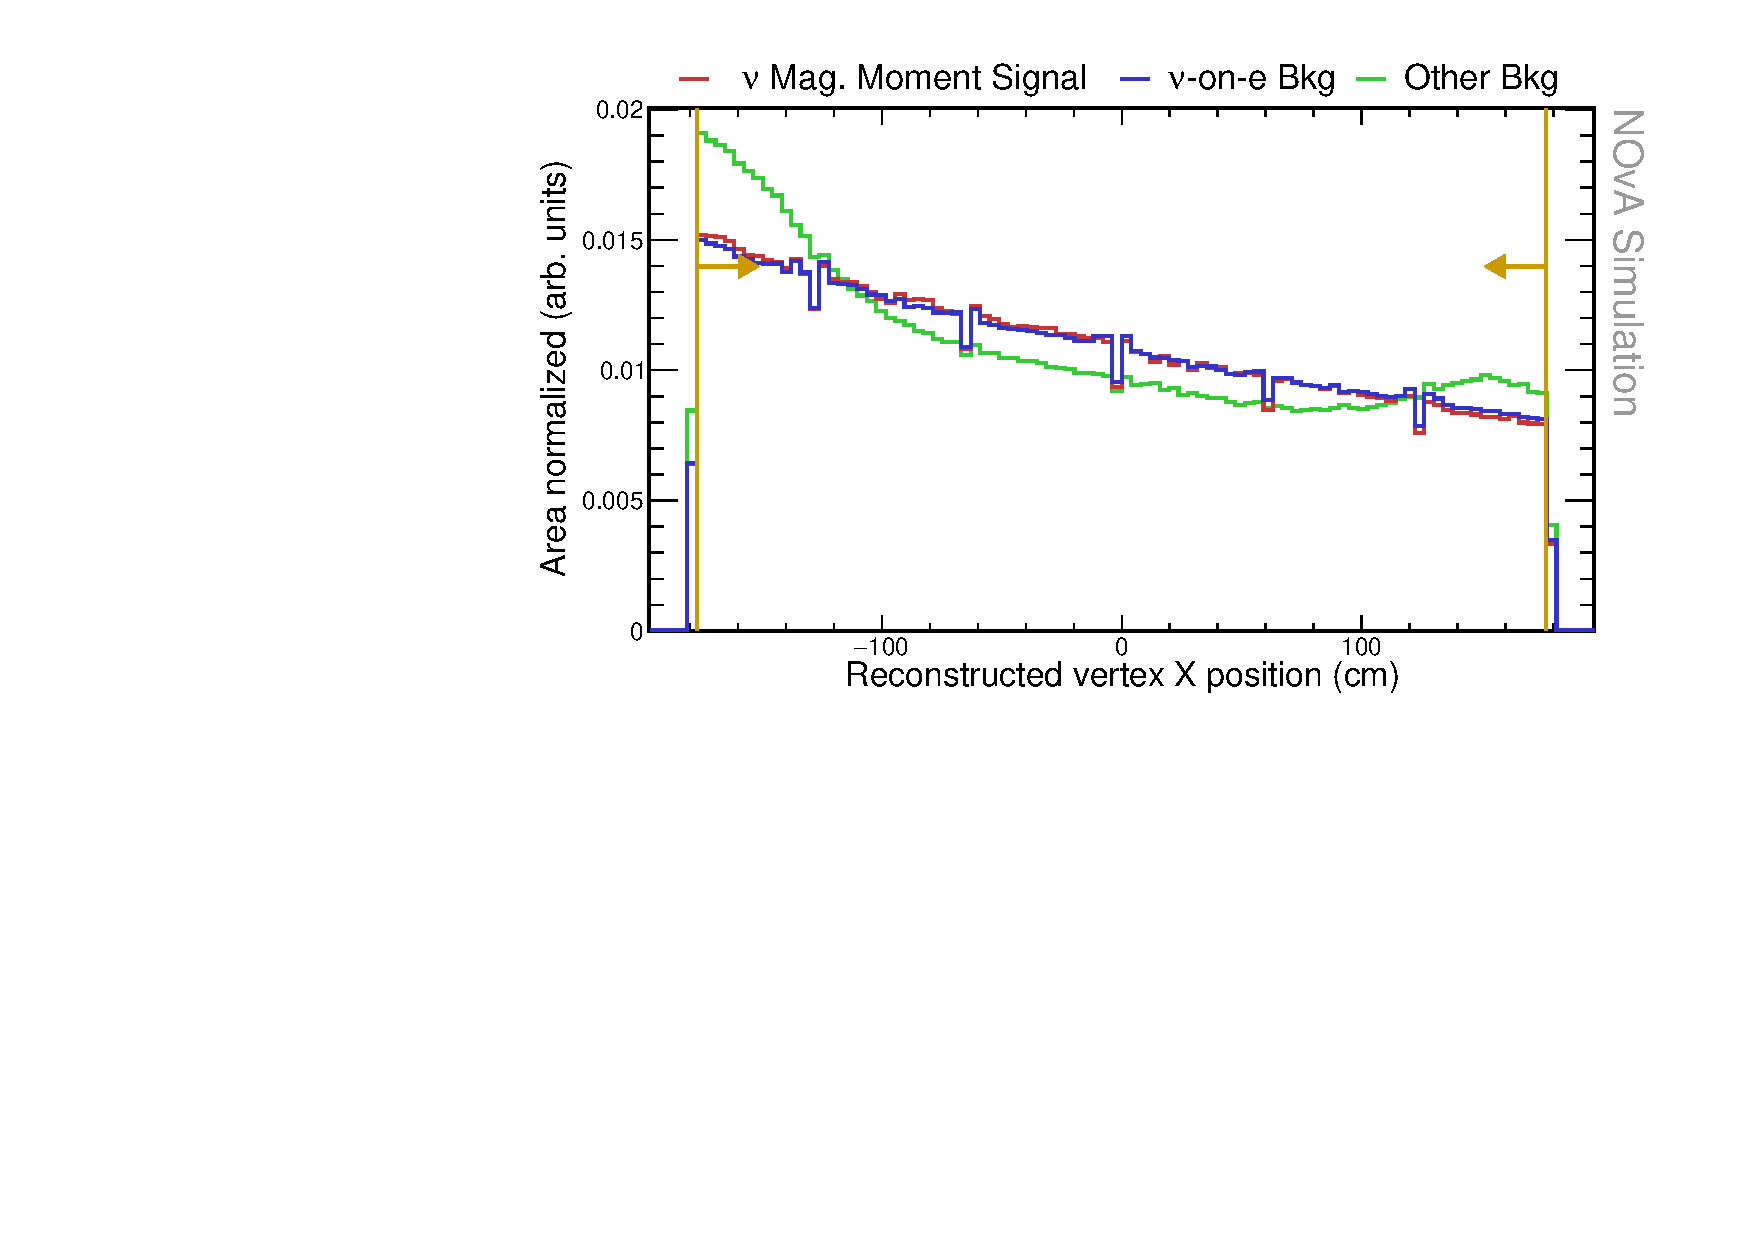
\includegraphics[width=.9\textwidth]{Plots/NuMMEventSelection/N1Cut_vtxXActive.pdf}
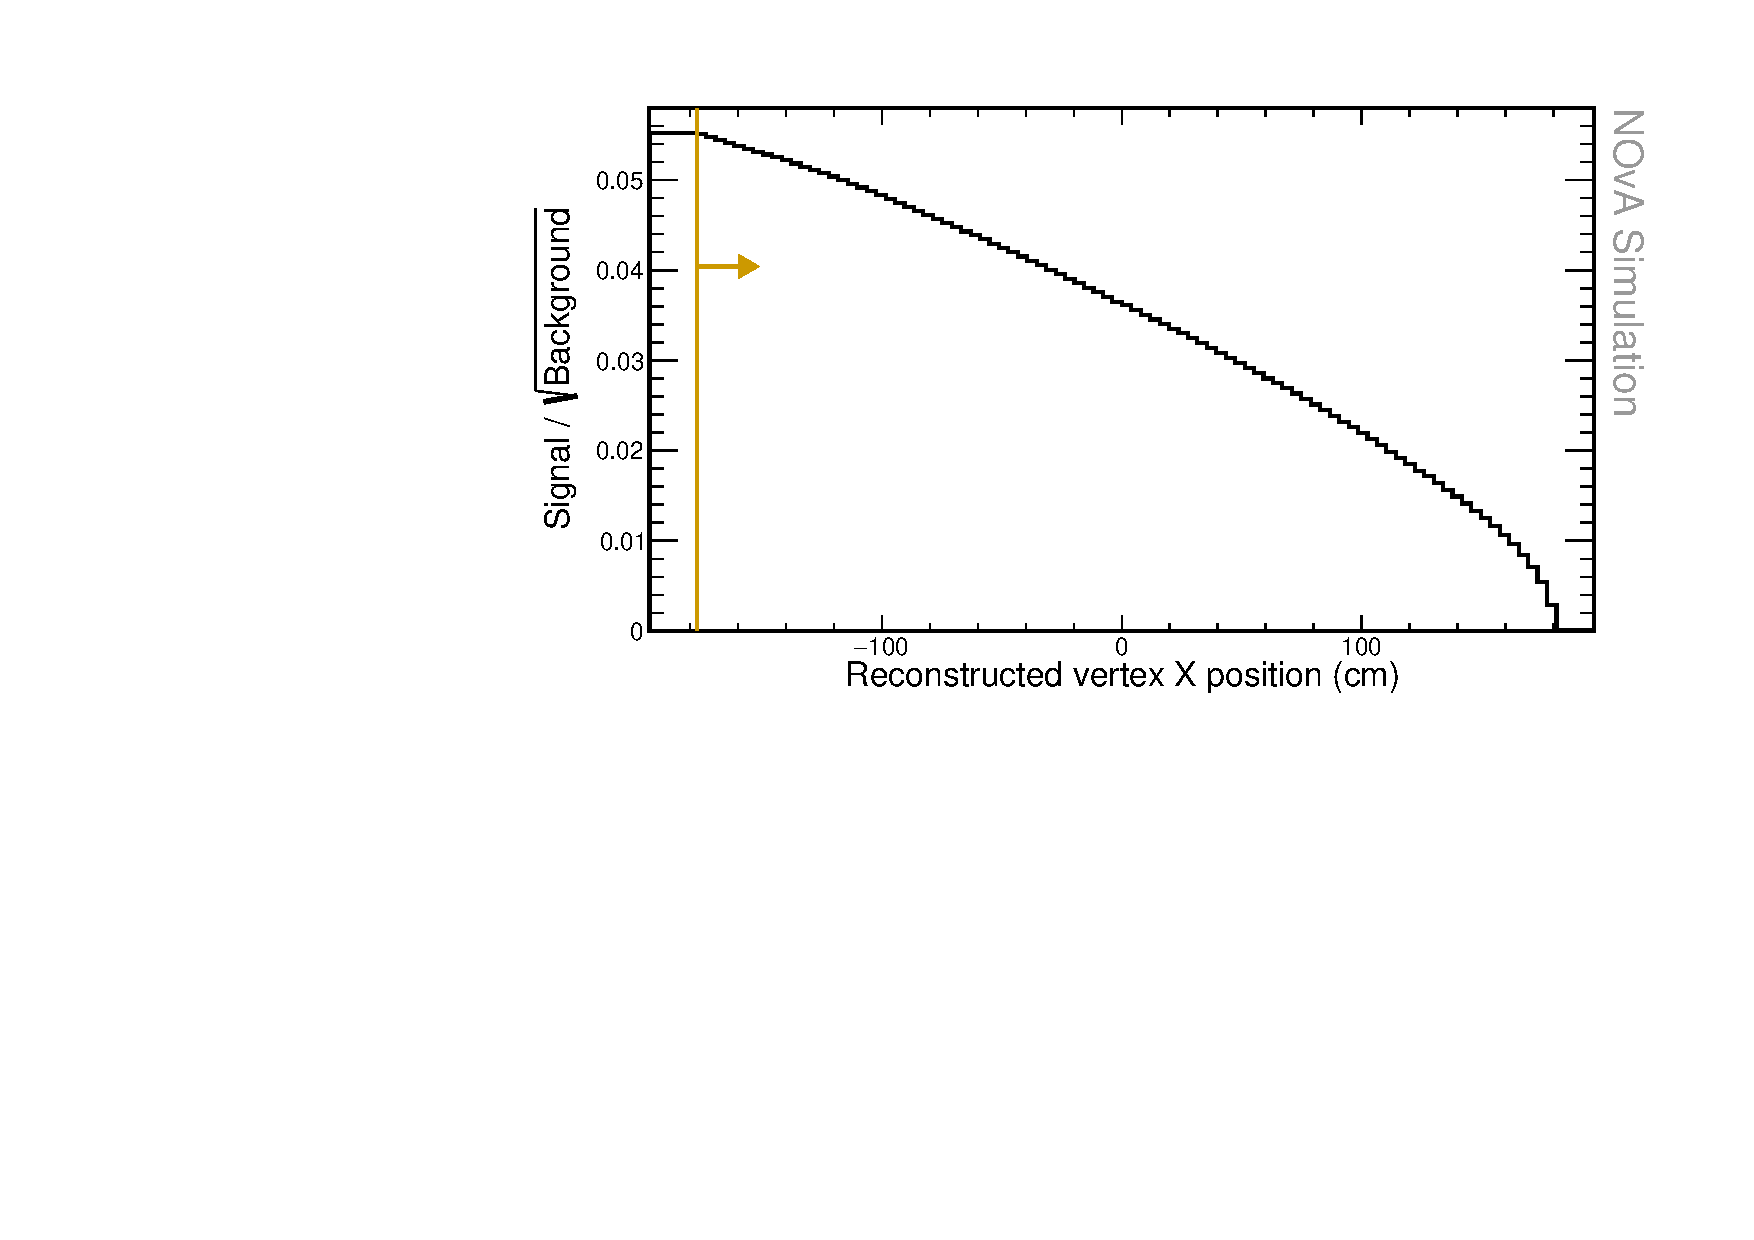
\includegraphics[width=.9\textwidth]{Plots/NuMMEventSelection/NuMM_N1Cut_vtxXActiveright_FOMStats.pdf}
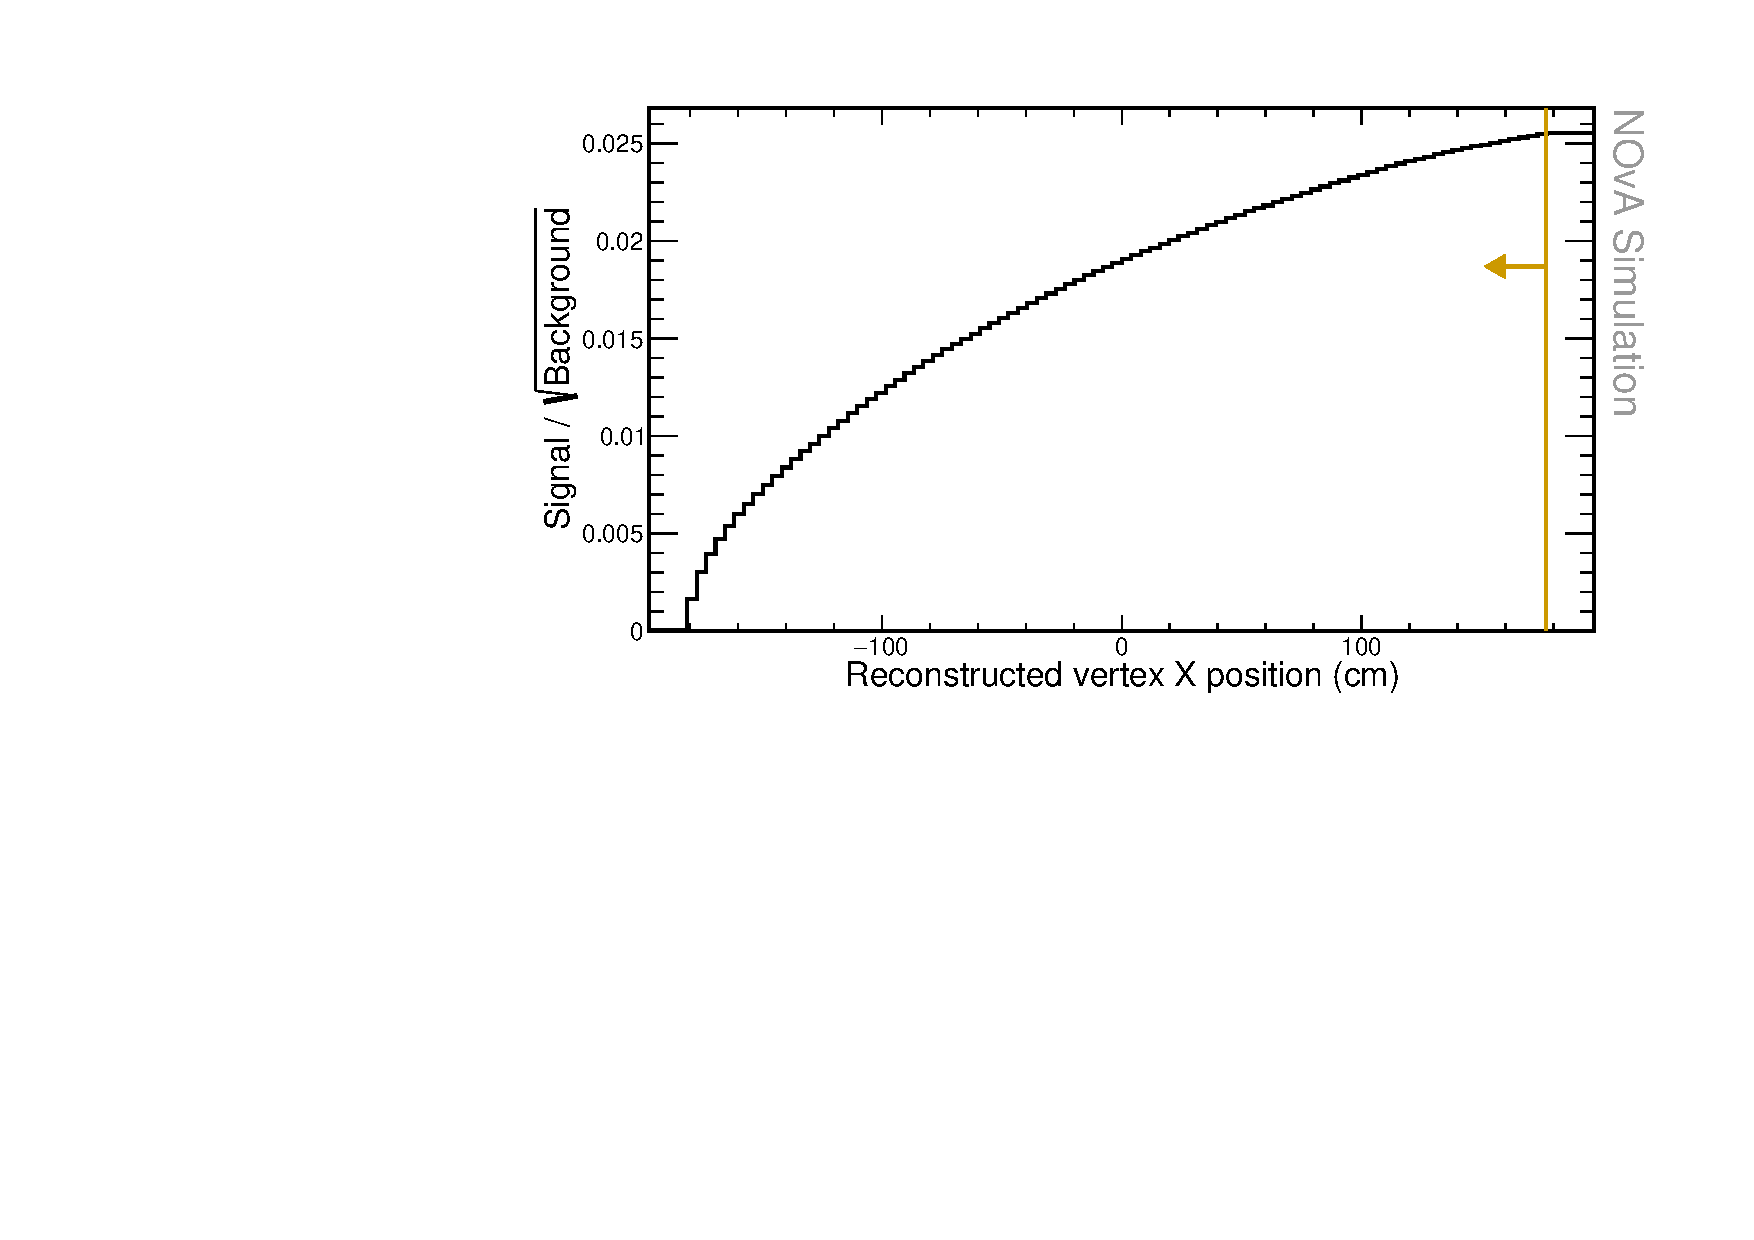
\includegraphics[width=.9\textwidth]{Plots/NuMMEventSelection/NuMM_N1Cut_vtxXActiveleft_FOMStats.pdf}
\caption[Vertex x containment cut]{Top: Relative comparison of signal (red), \acrshort{nuone} background (blue), and other background (green) events in the distribution of the x position of the reconstructed vertex. All histograms are area-normalized. Middle and bottom: Cumulative \acrshort{FOM} calculated as the number of signal events, divided by the number of background events from that bin until the end of the plot in the direction of the yellow arrow. The reconstruction quality and basic selection cuts were applied prior to making these plots. Additionally, vertex is required to be within the active region of the detector ($Vtx_Z<\unit[1270]{cm}$). Yellow lines show the cut values that create the fiducial volume, with arrows pointing towards the preserved events.}
\label{fig:NuMMFiducialCutX}
\end{figure}

\begin{figure}[hbtp]
\centering
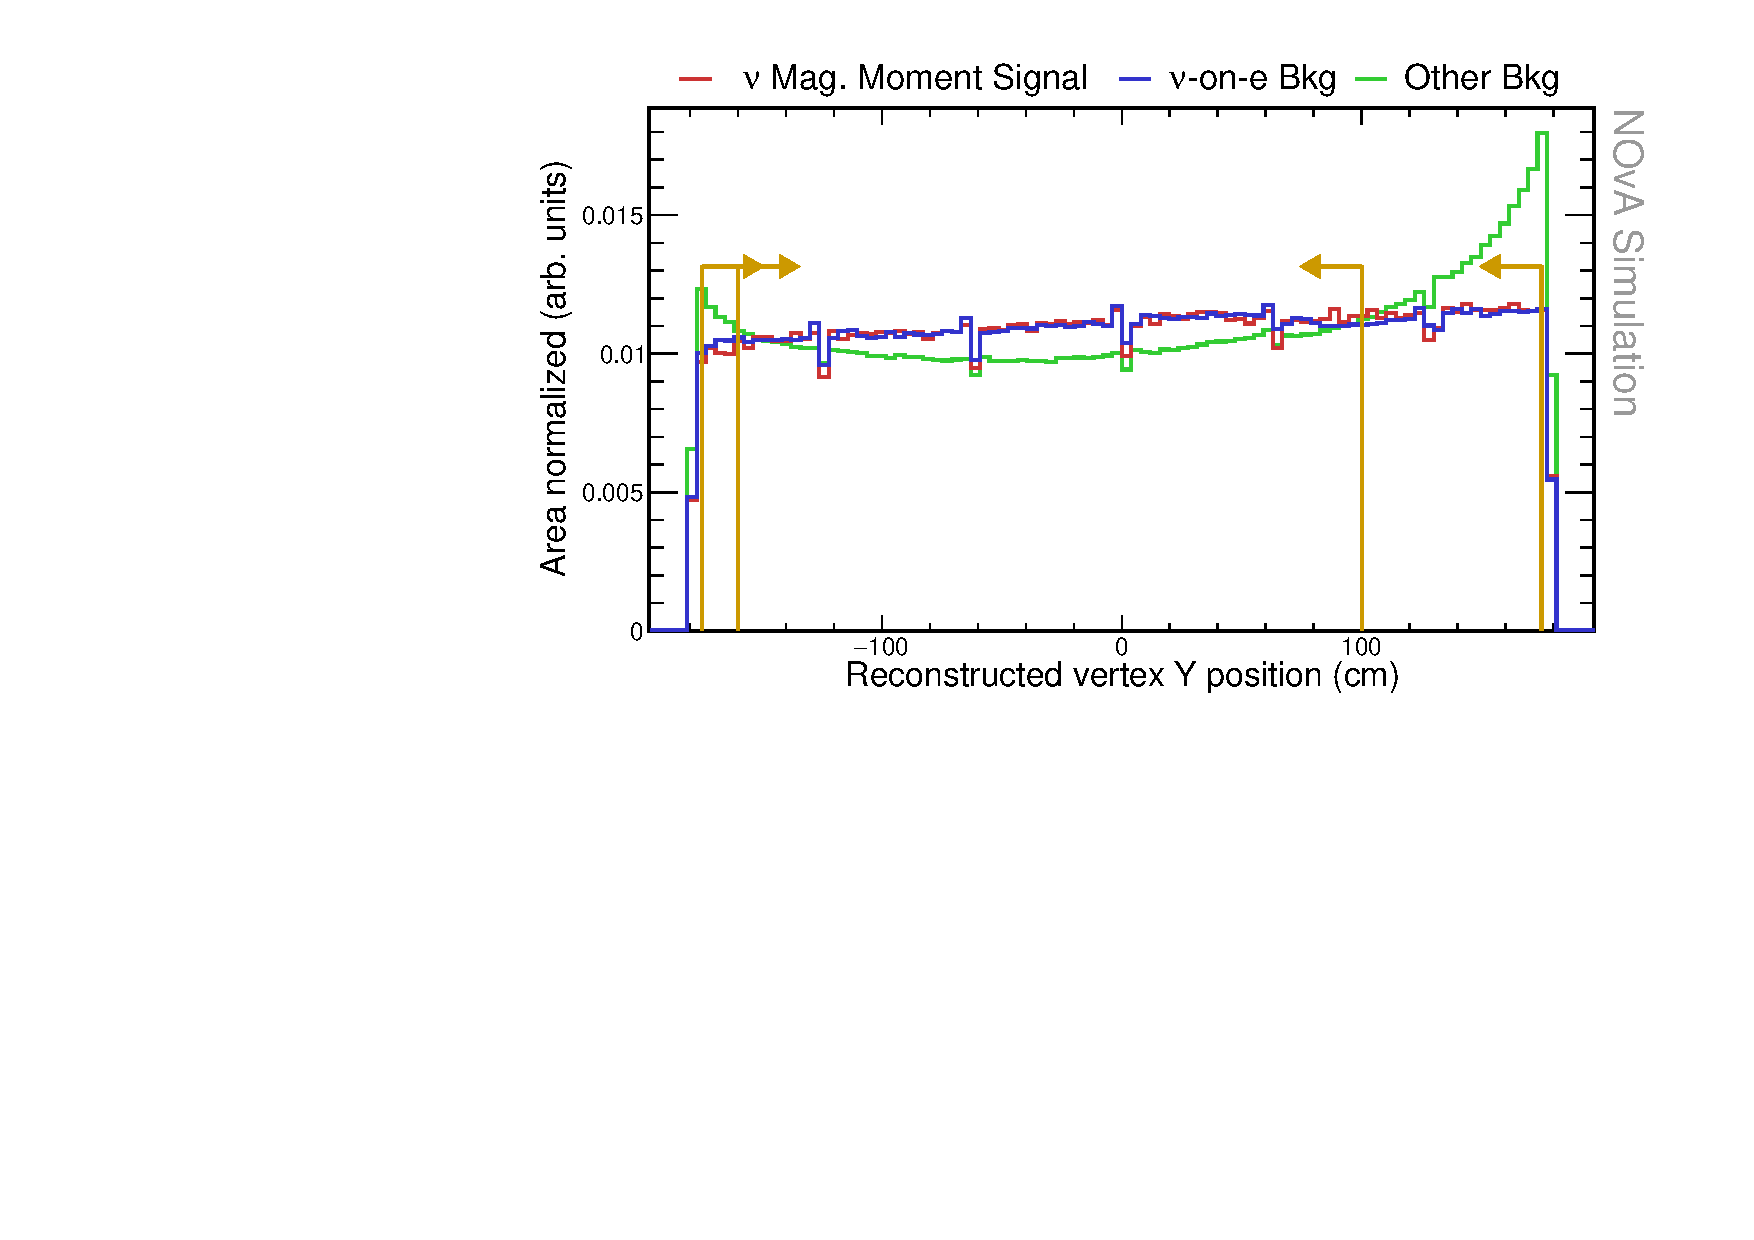
\includegraphics[width=.9\textwidth]{Plots/NuMMEventSelection/N1Cut_vtxYActive.pdf}
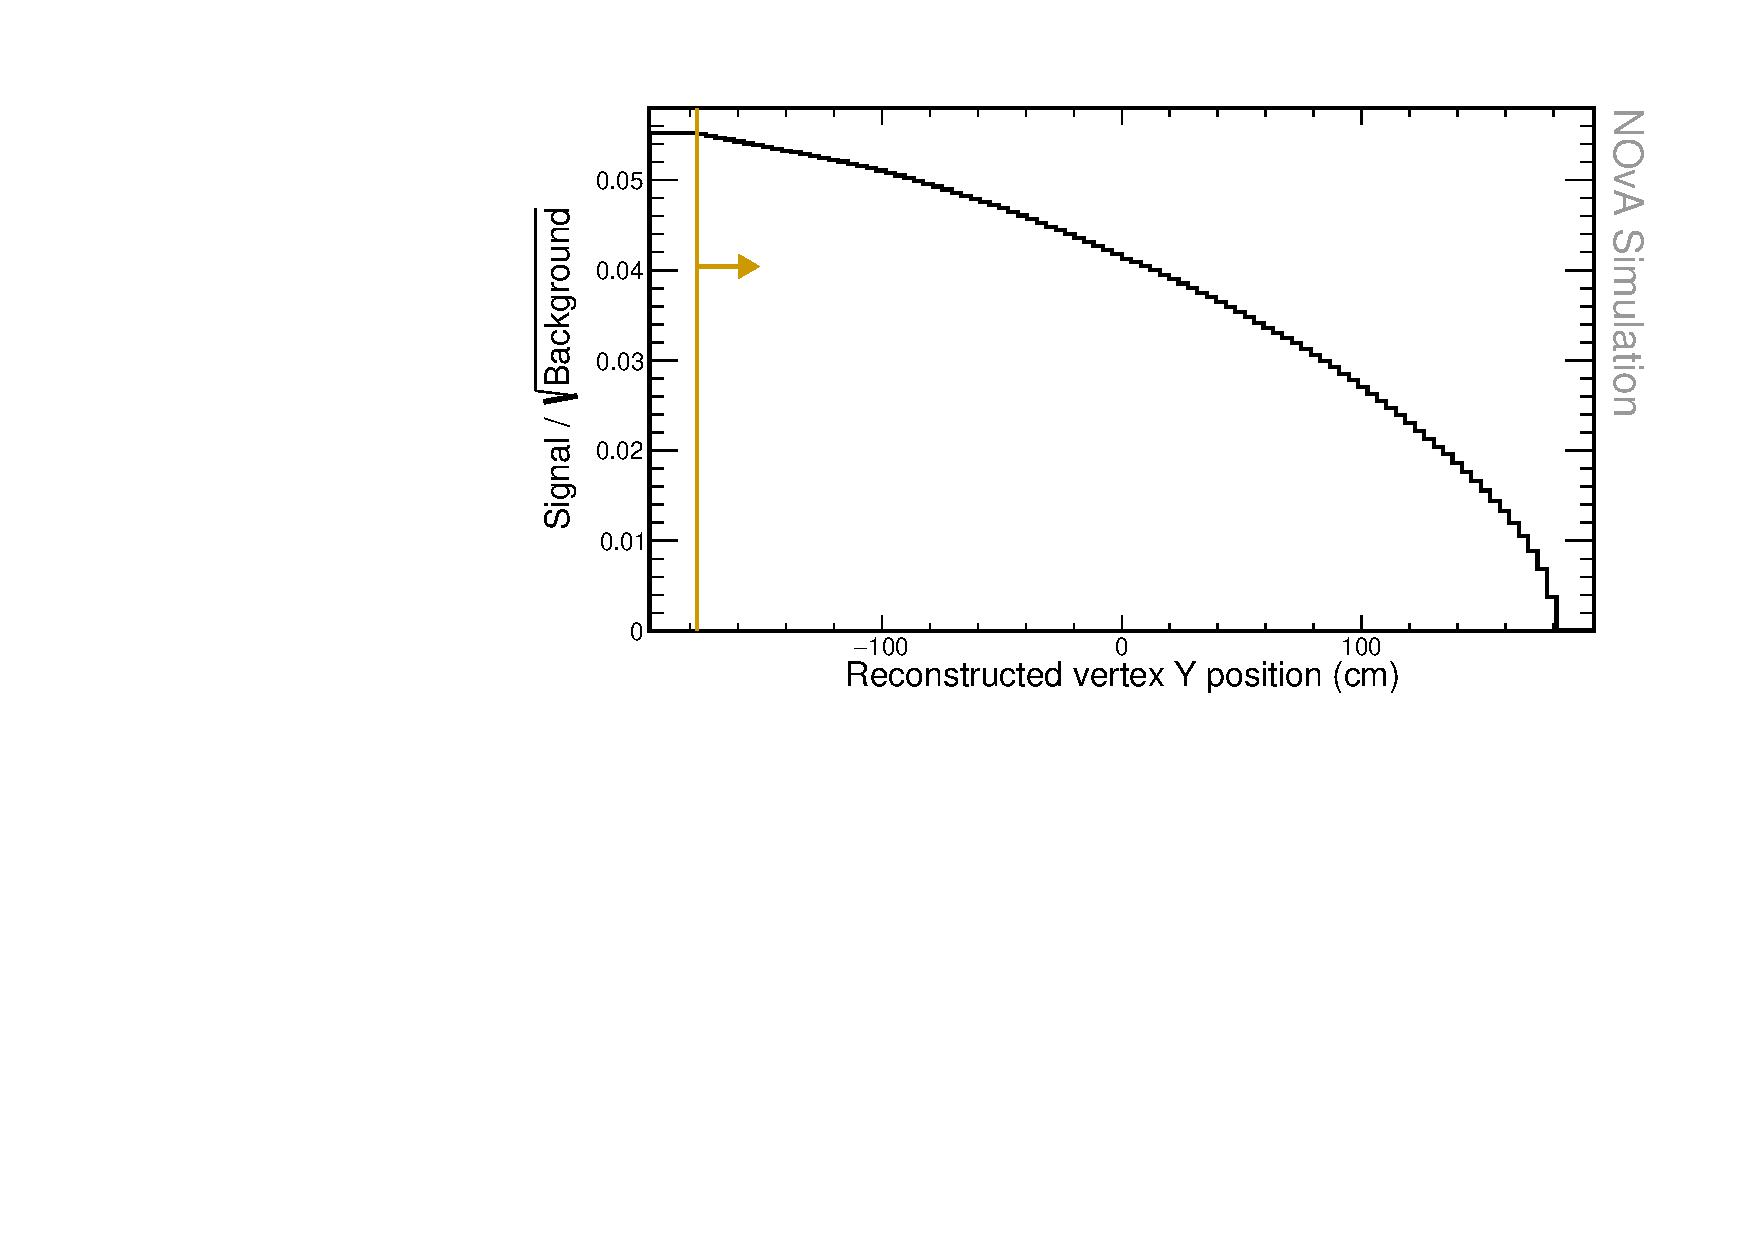
\includegraphics[width=.9\textwidth]{Plots/NuMMEventSelection/NuMM_N1Cut_vtxYActiveright_FOMStats.pdf}
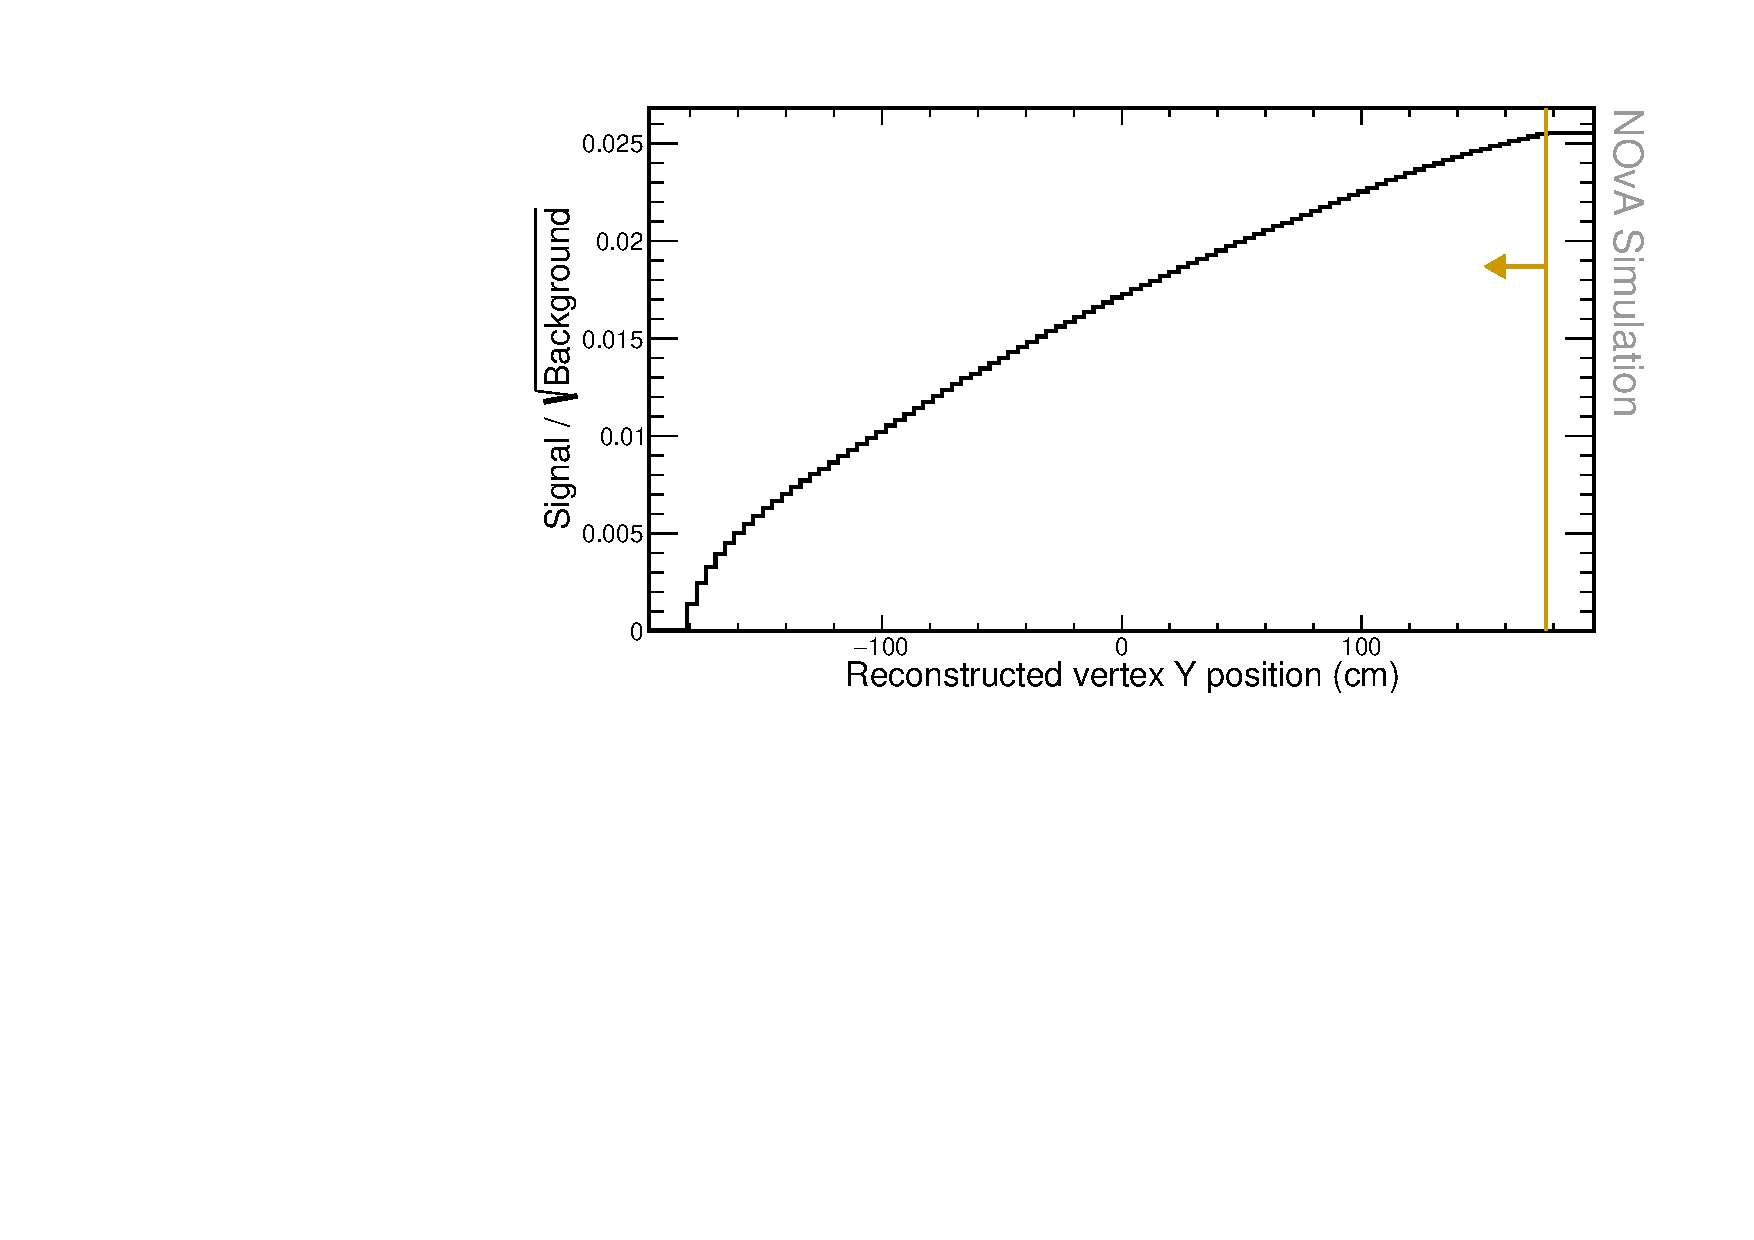
\includegraphics[width=.9\textwidth]{Plots/NuMMEventSelection/NuMM_N1Cut_vtxYActiveleft_FOMStats.pdf}
\caption[Vertex y containment cut]{Top: Relative comparison of signal (red), \acrshort{nuone} background (blue), and other background (green) events in the distribution of the y position of the reconstructed vertex. All histograms are area-normalized. Middle and bottom: Cumulative \acrshort{FOM} calculated as the number of signal events, divided by the number of background events from that bin until the end of the plot in the direction of the yellow arrow. The reconstruction quality and basic selection cuts were applied prior to making these plots. Additionally, vertex is required to be within the active region of the detector ($Vtx_Z<\unit[1270]{cm}$). Yellow lines show the cut values that create the fiducial volume, with arrows pointing towards the preserved events.}
\label{fig:NuMMFiducialCutY}
\end{figure}

\begin{figure}[hbtp]
\centering
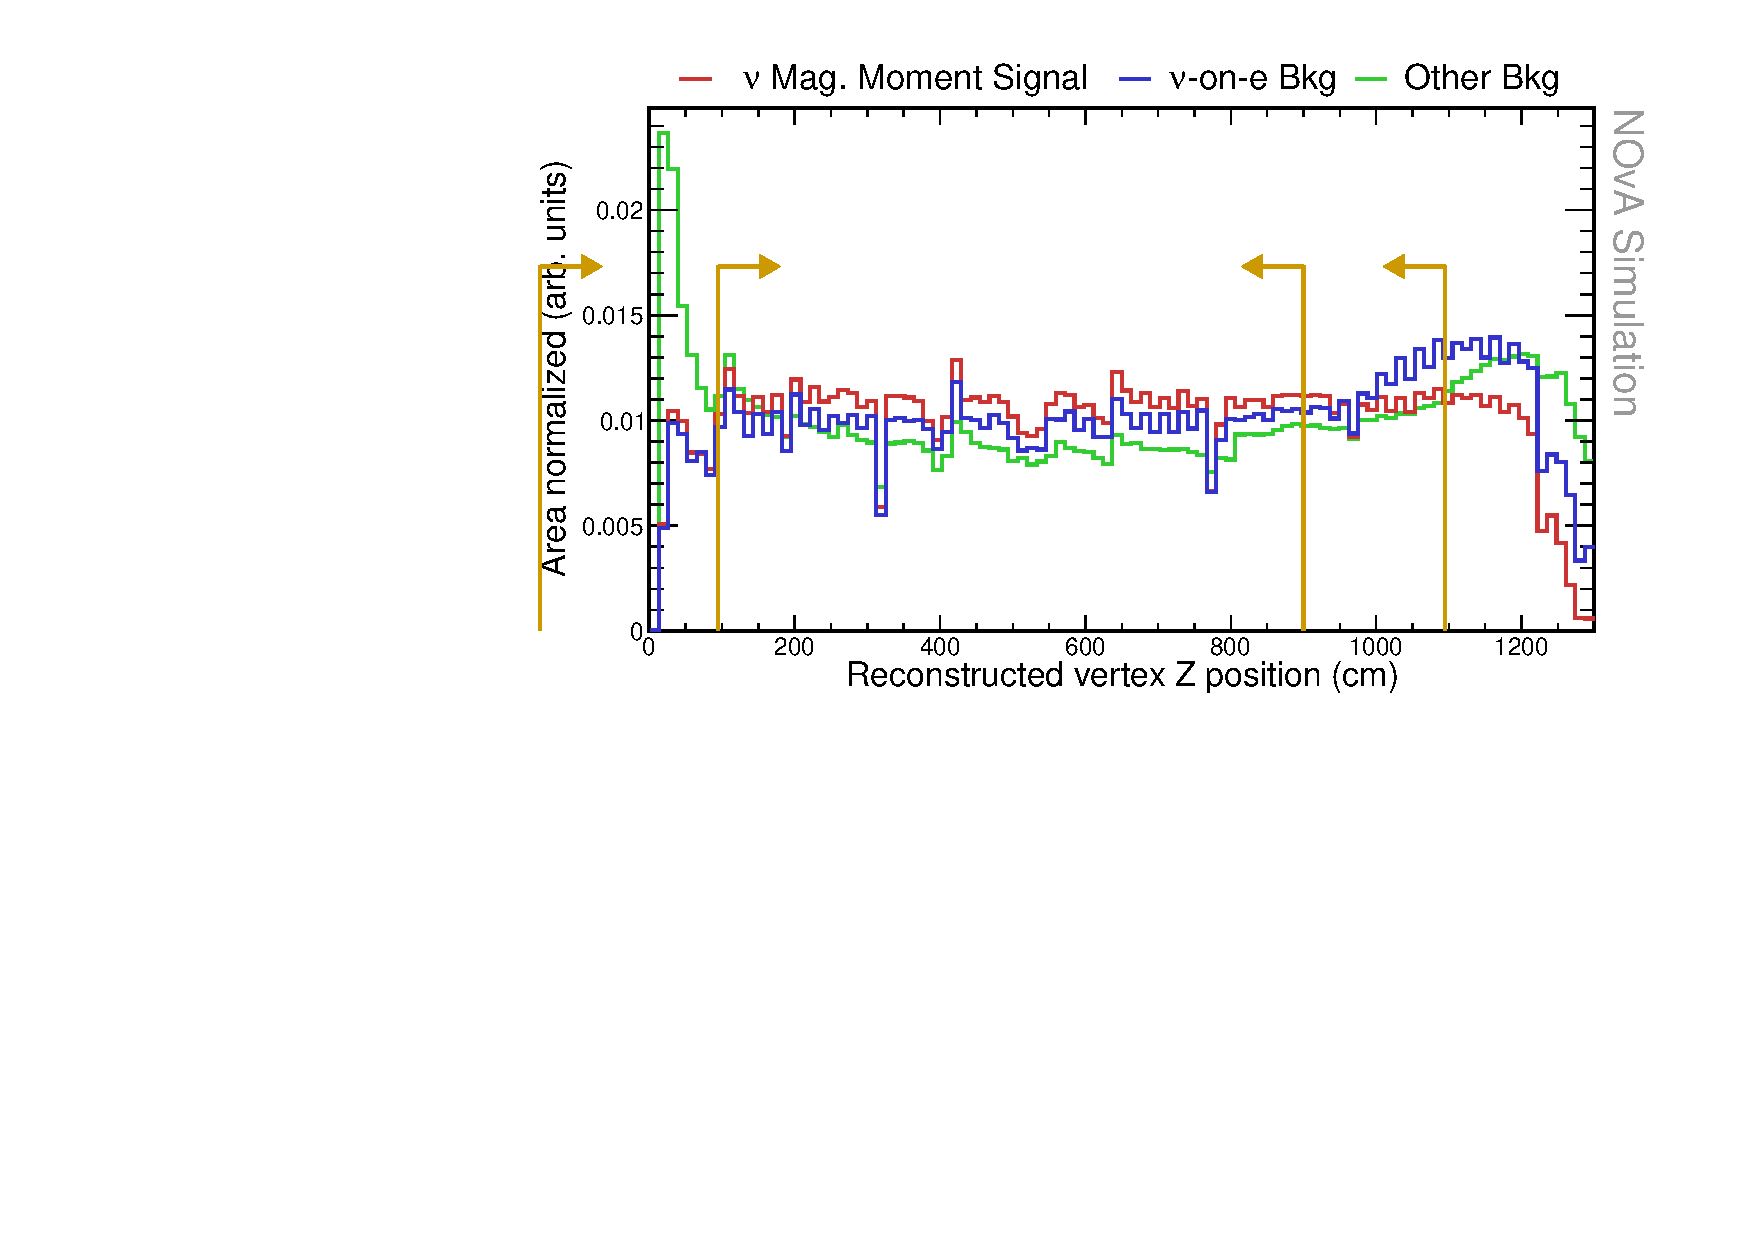
\includegraphics[width=.9\textwidth]{Plots/NuMMEventSelection/N1Cut_vtxZ.pdf}
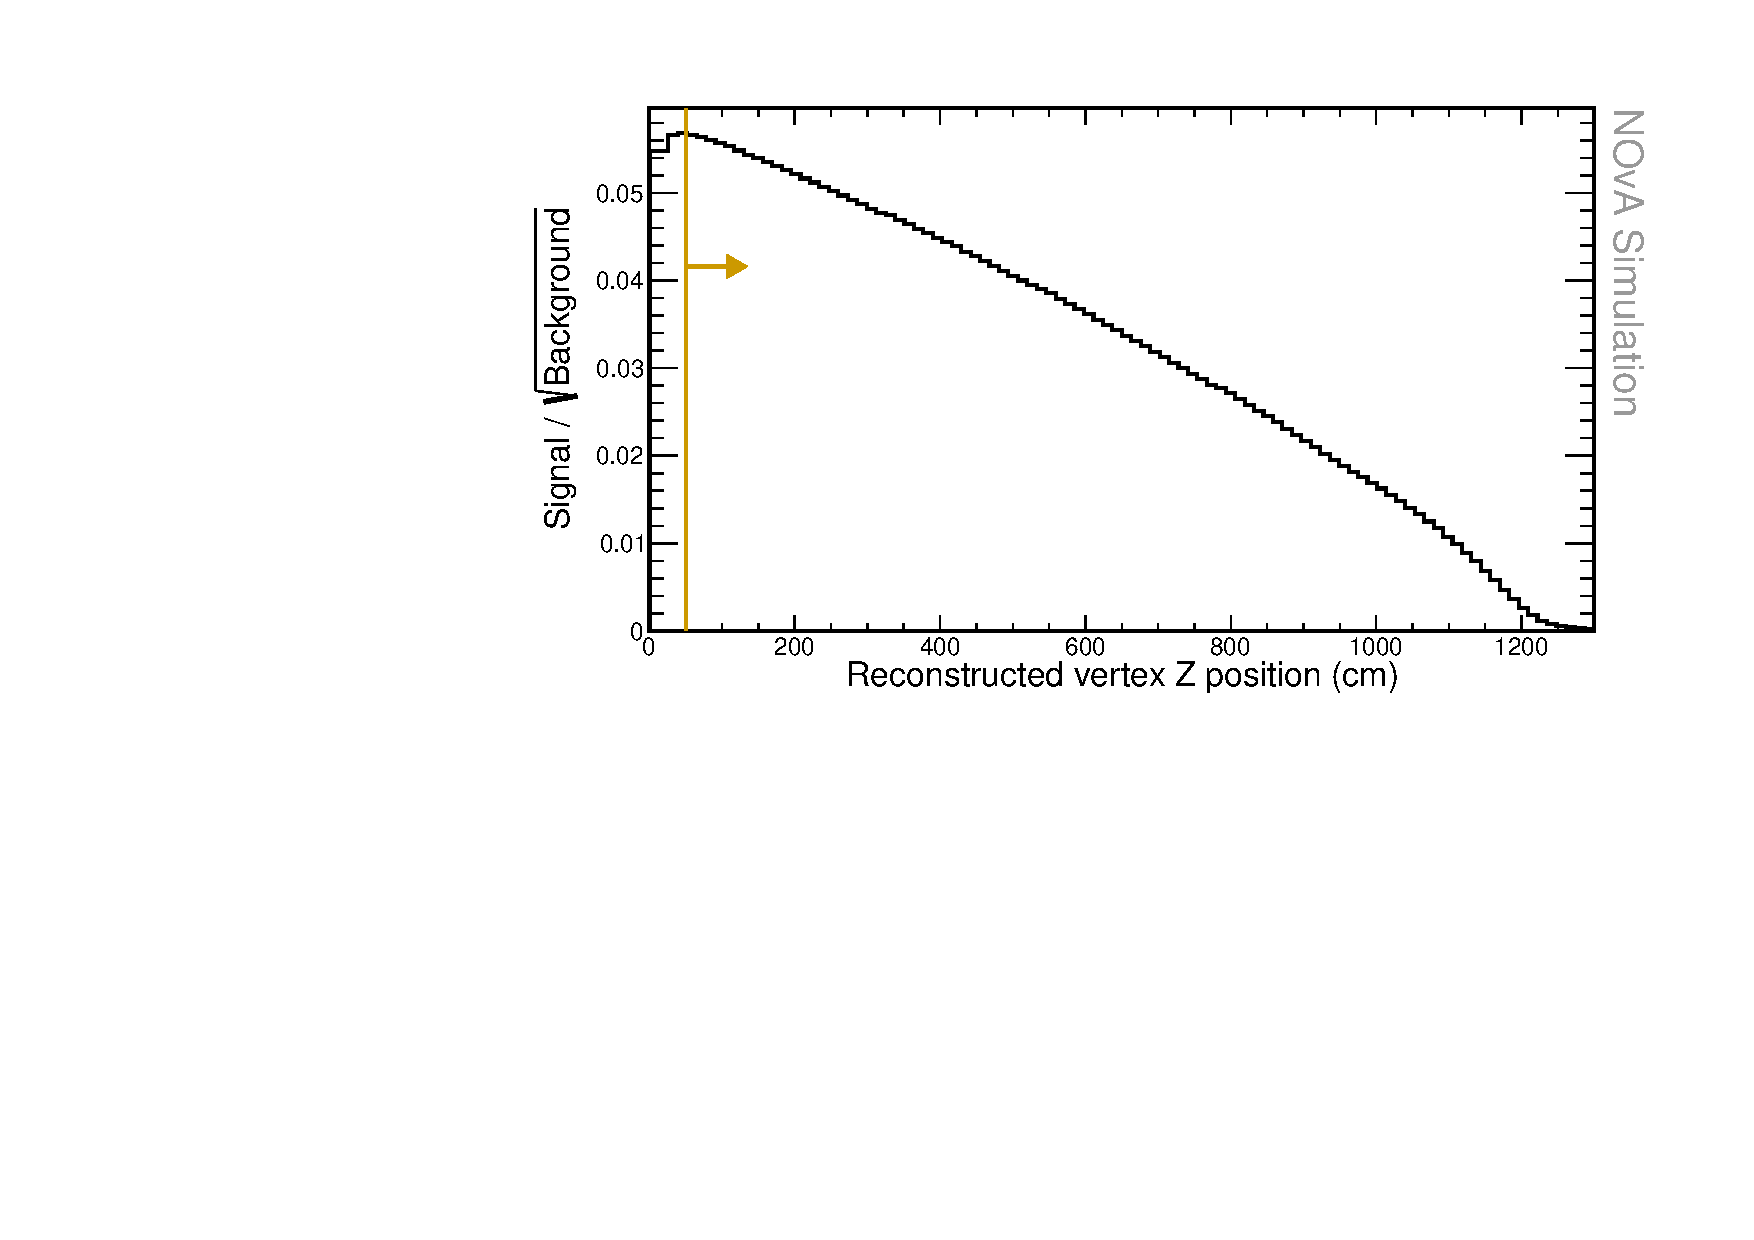
\includegraphics[width=.9\textwidth]{Plots/NuMMEventSelection/NuMM_N1Cut_vtxZright_FOMStats.pdf}
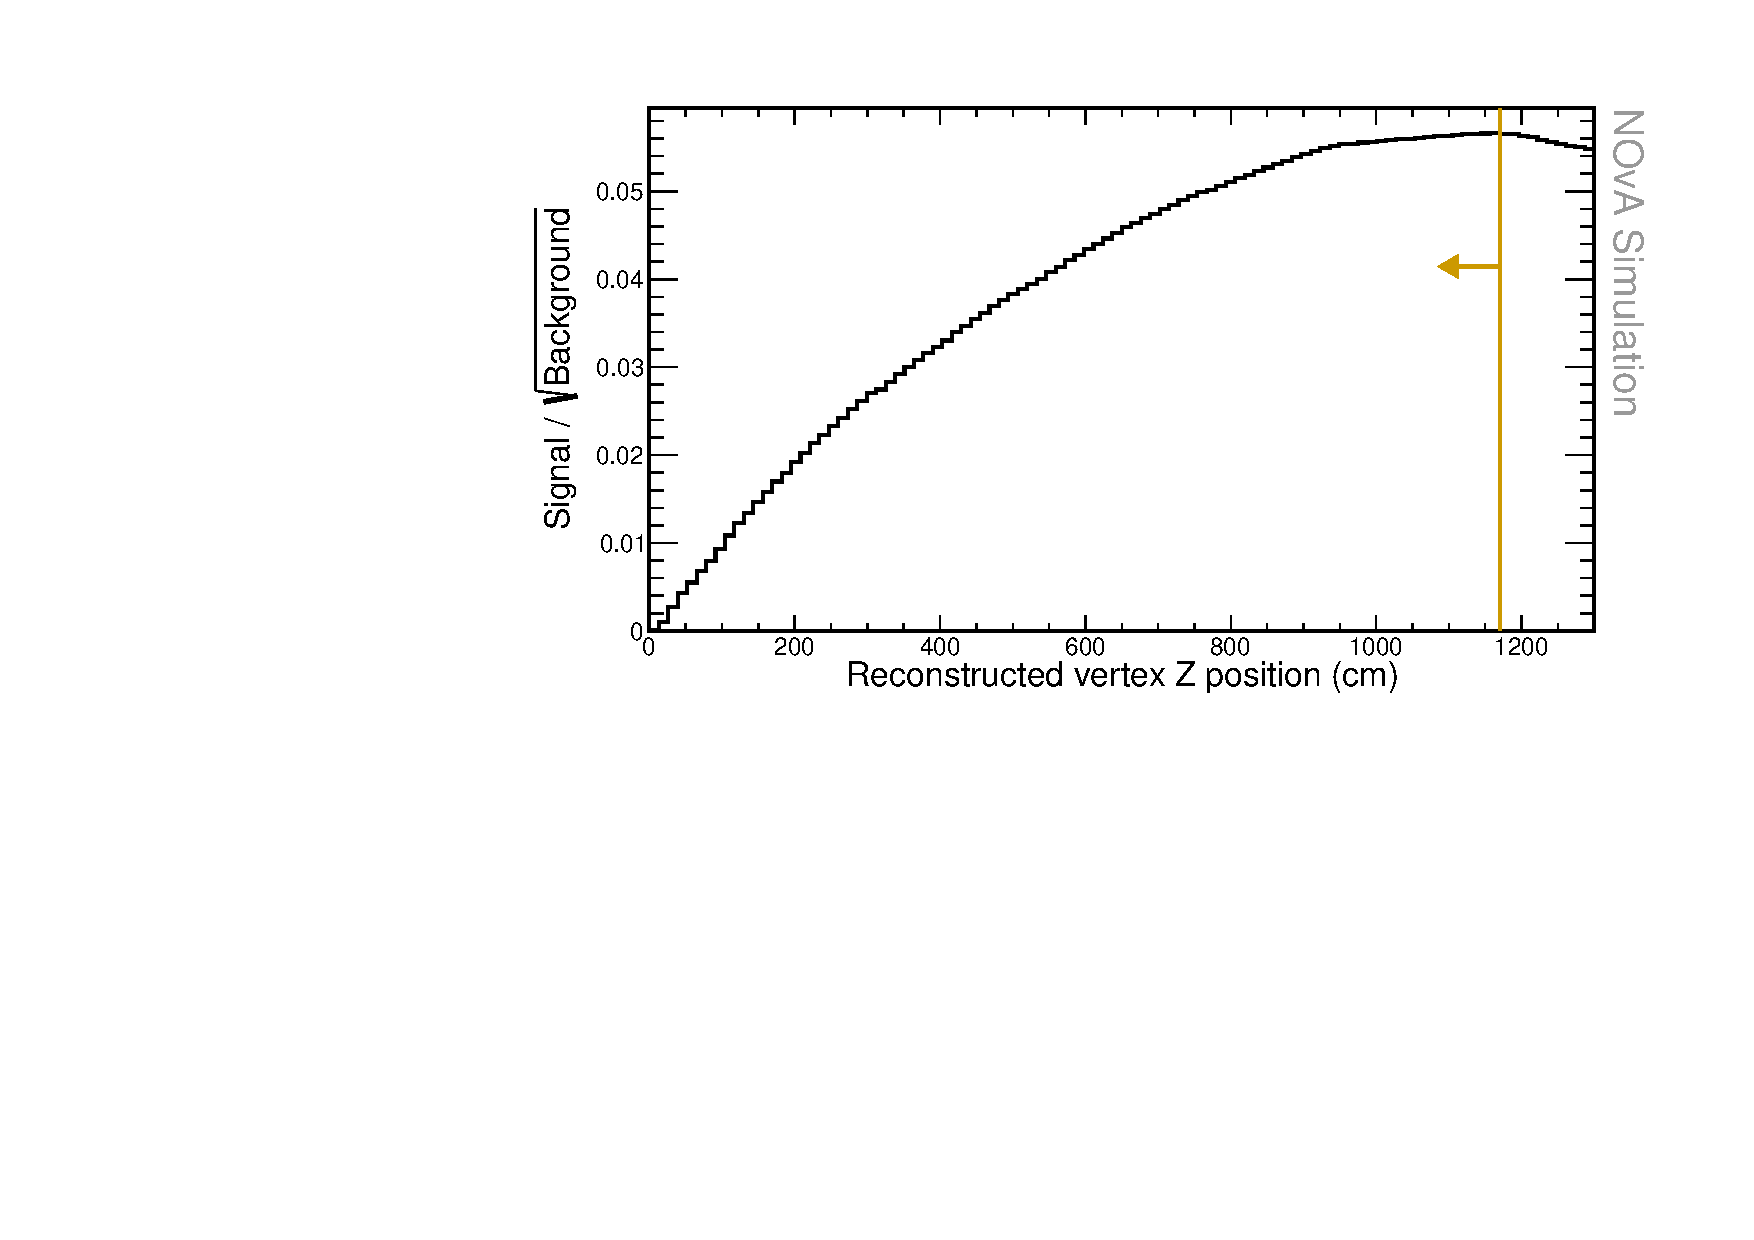
\includegraphics[width=.9\textwidth]{Plots/NuMMEventSelection/NuMM_N1Cut_vtxZleft_FOMStats.pdf}
\caption[Vertex z containment cut]{Top: Relative comparison of signal (red), \acrshort{nuone} background (blue), and other background (green) events in the distribution of the z position of the reconstructed vertex. All histograms are area-normalized. Middle and bottom: Cumulative \acrshort{FOM} calculated as the number of signal events, divided by the number of background events from that bin until the end of the plot in the direction of the yellow arrow. The reconstruction quality and basic selection cuts were applied prior to making these plots. Yellow lines show the cut values that create the fiducial volume, with arrows pointing towards the preserved events.}
\label{fig:NuMMFiducialCutY}
\end{figure}

To ensure all the energy is contained within the detector and to remove events originating outside of the detector (rock muons), we require that the extreme positions of hits for all prongs in the slice are within the following volume: $-175<\textsf{min}_X, \textsf{max}_X<175, -175<\textsf{min}_Y, \textsf{max}_Y<175, 105<\textsf{min}_Z, \textsf{max}_Z<1270\ \unit{cm}$. \note{Also made this a bit stricter from the ND group's values as it didn't really make sense}

\begin{figure}[hbtp]
\centering
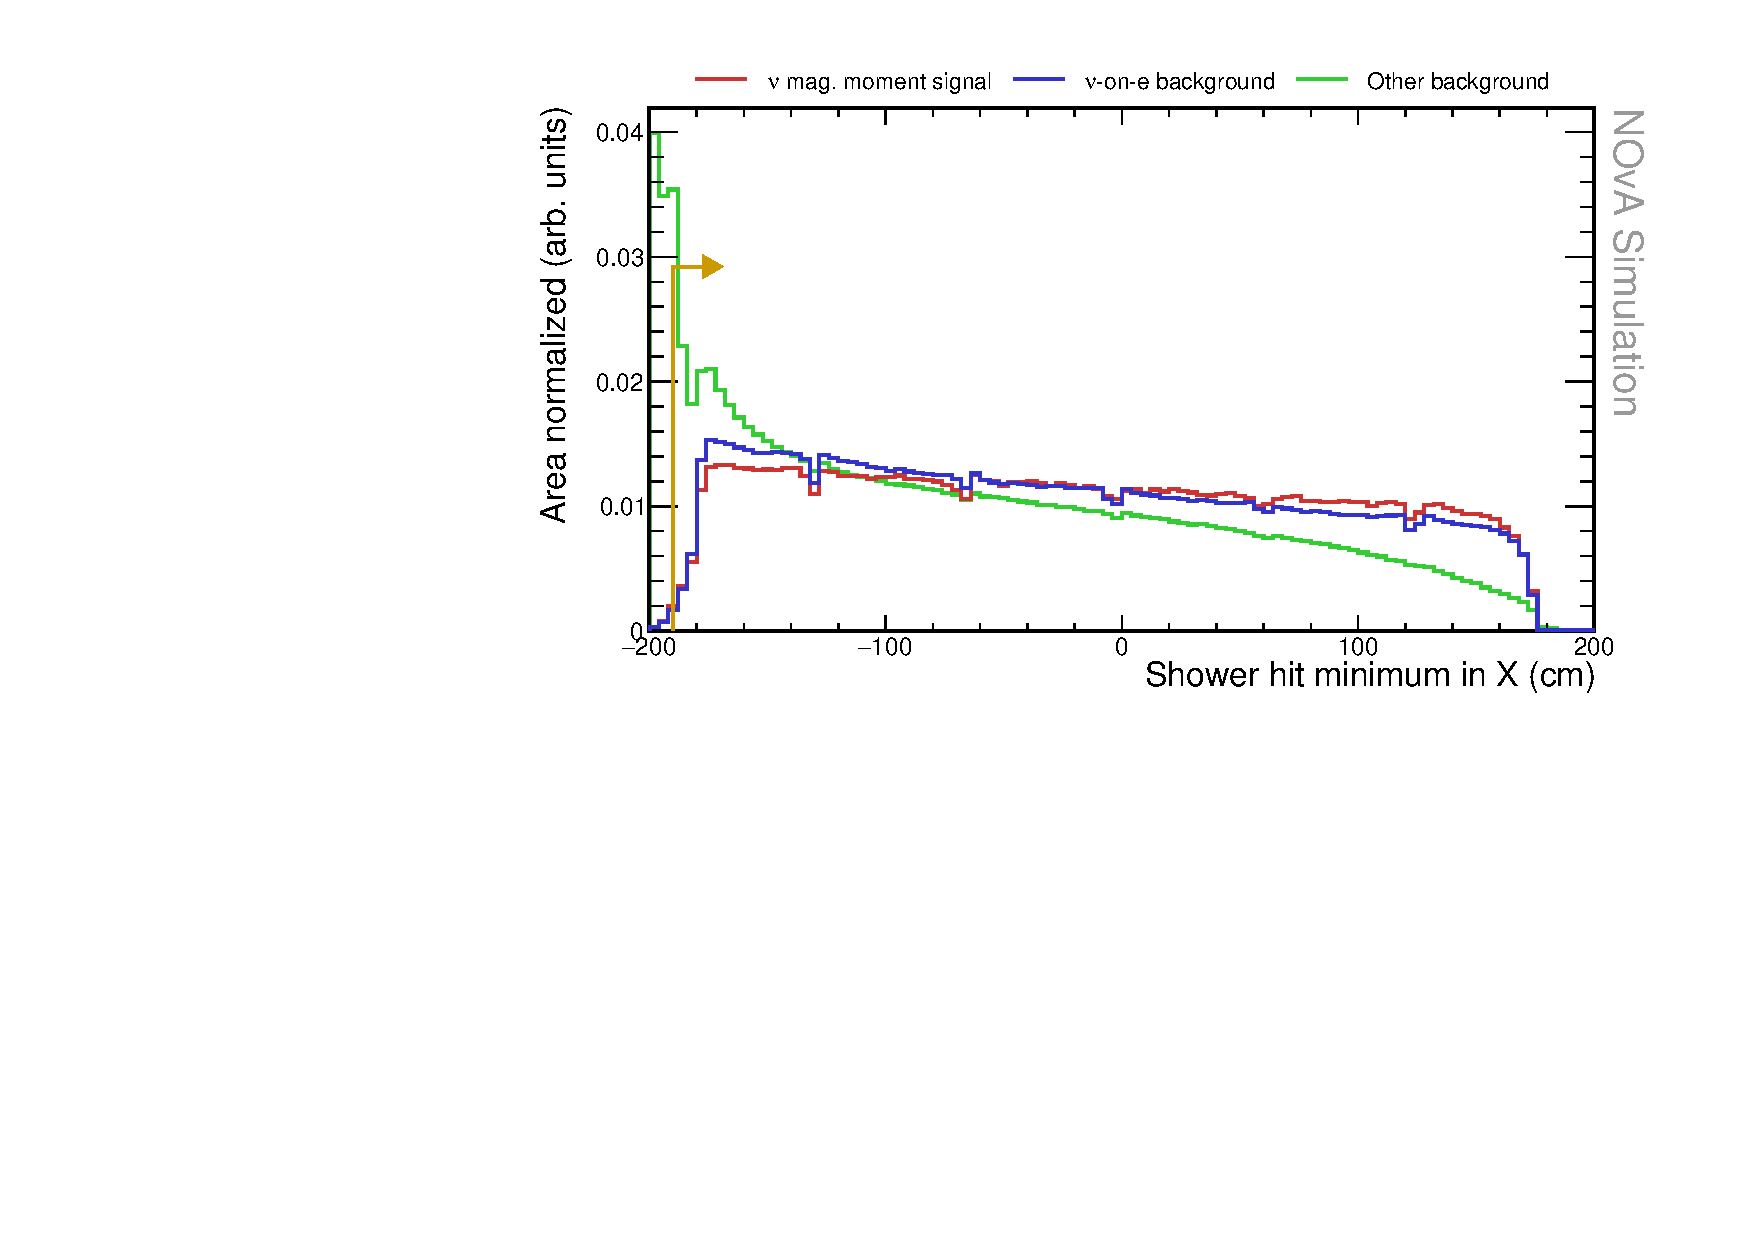
\includegraphics[width=.9\textwidth]{Plots/NuMMEventSelection/N1Cut_minX.pdf}
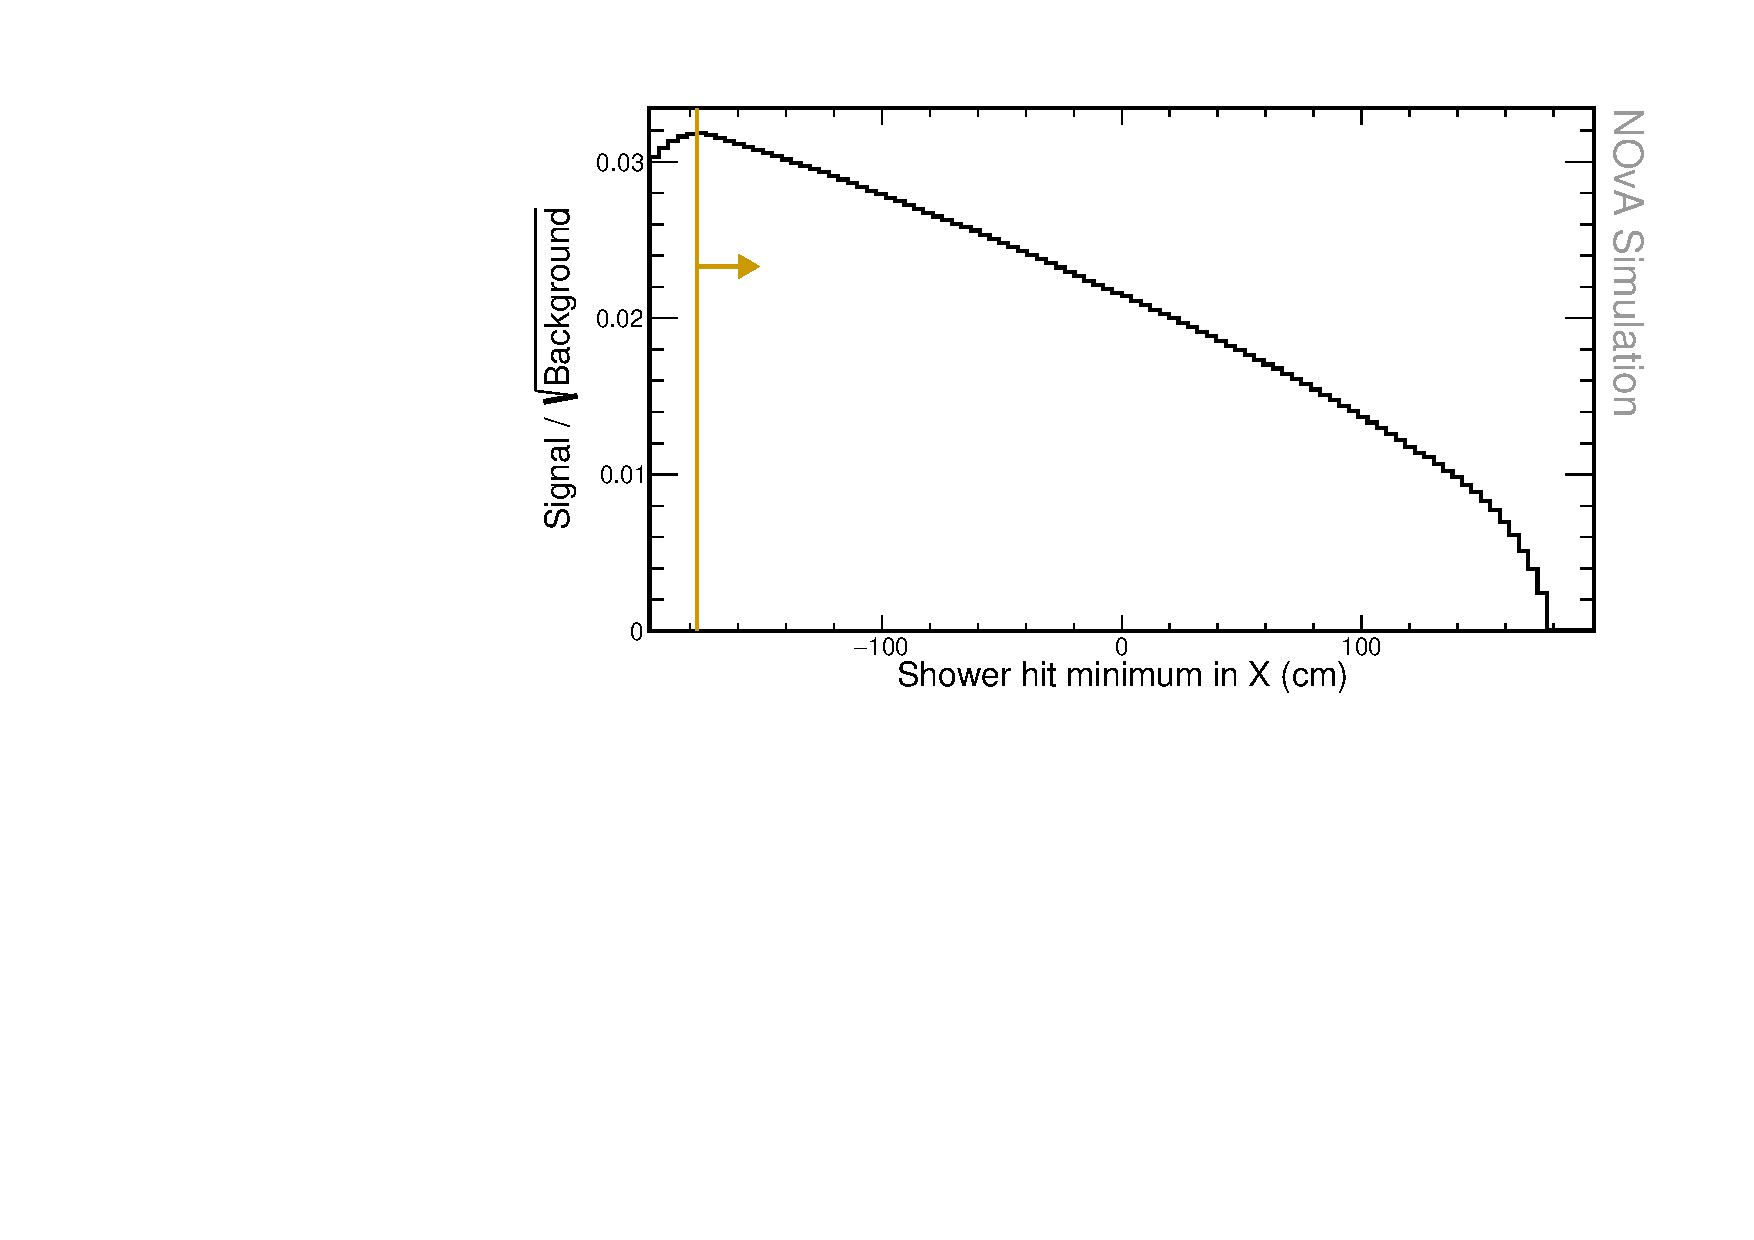
\includegraphics[width=.9\textwidth]{Plots/NuMMEventSelection/NuMM_N1Cut_minXright_FOMStats.pdf}
\caption{Relative comparison of signal, \acrshort{nuone} background, and other background events for the minimum and maximum position of the reconstructed shower along the x axis. Pre-selection and fiducial cuts were applied to make these plots. Gold lines show the values of the containment cuts.}
\label{fig:NuMMContainmentCutMinX}
\end{figure}

\begin{figure}[hbtp]
\centering
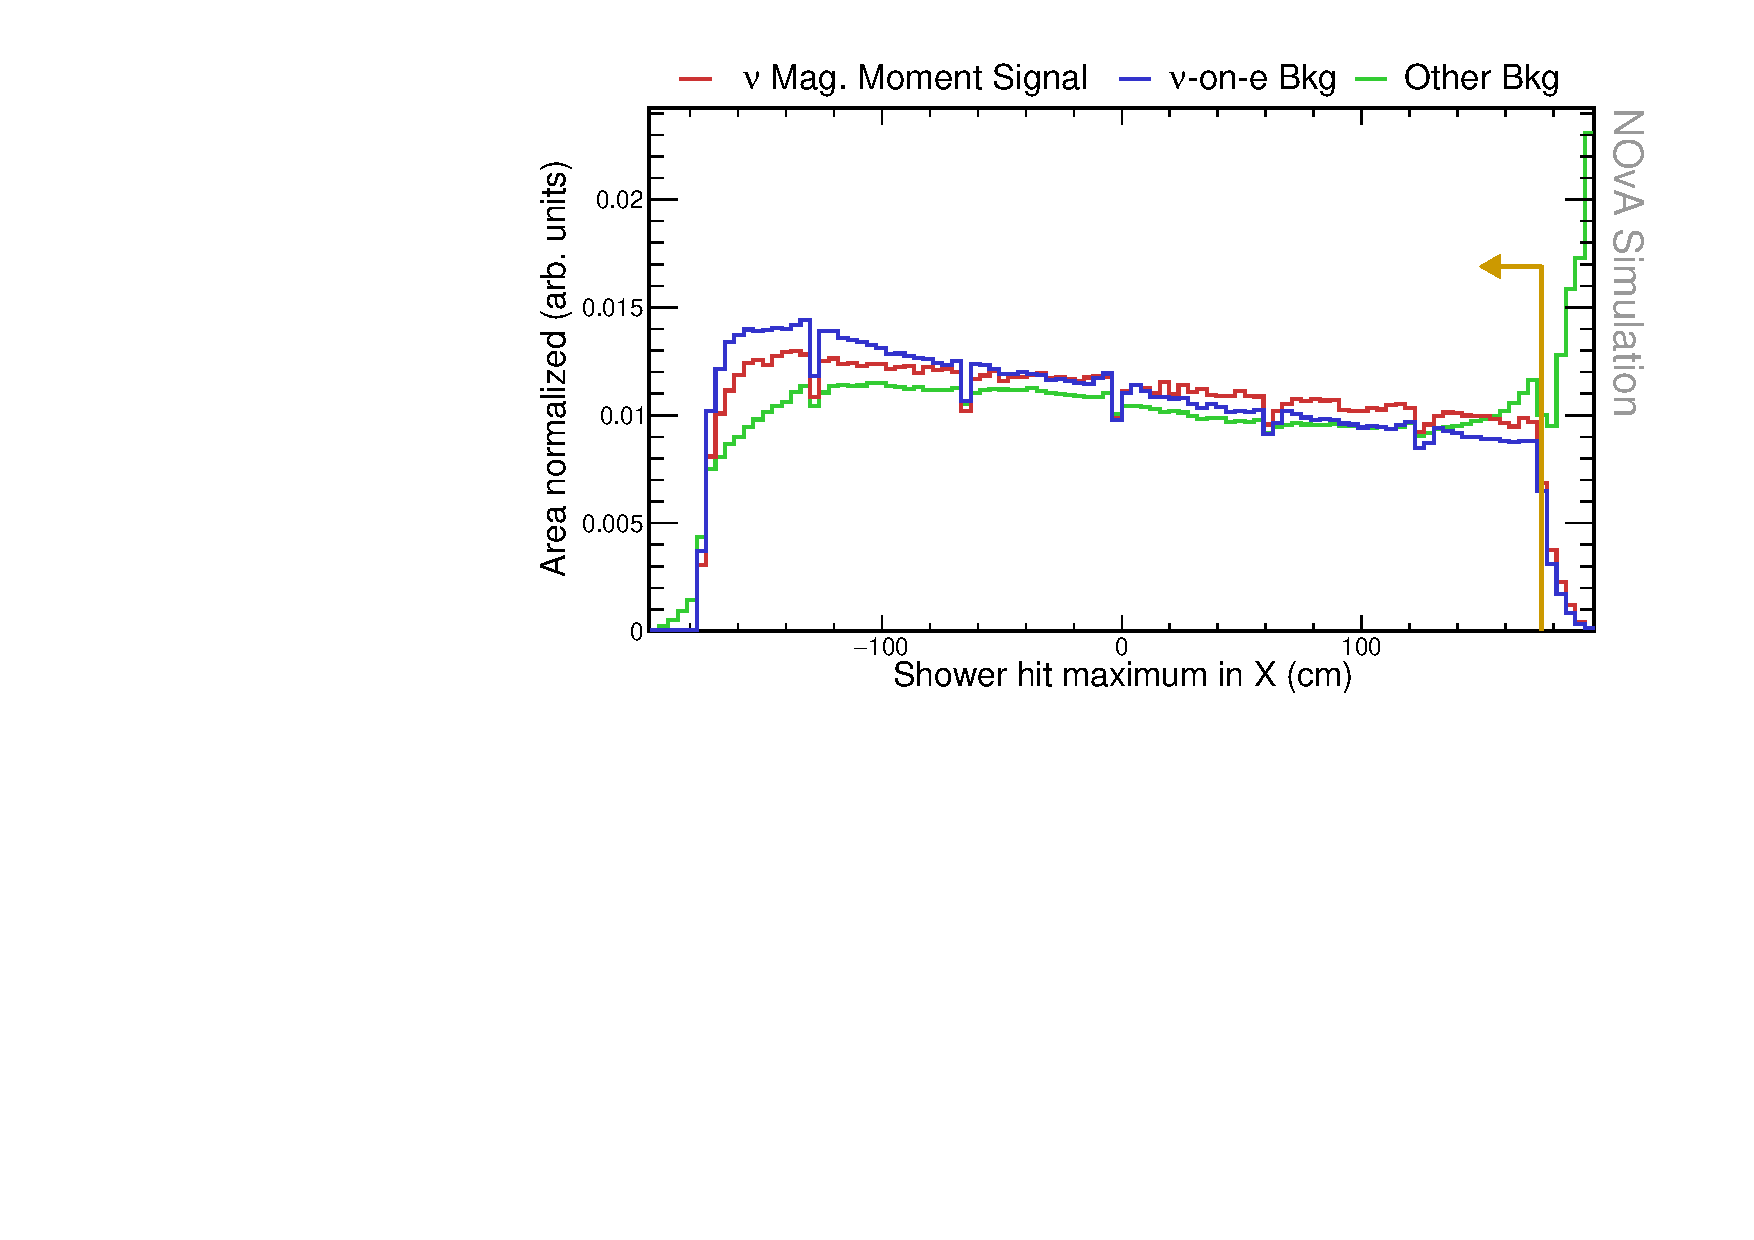
\includegraphics[width=.9\textwidth]{Plots/NuMMEventSelection/N1Cut_maxX.pdf}
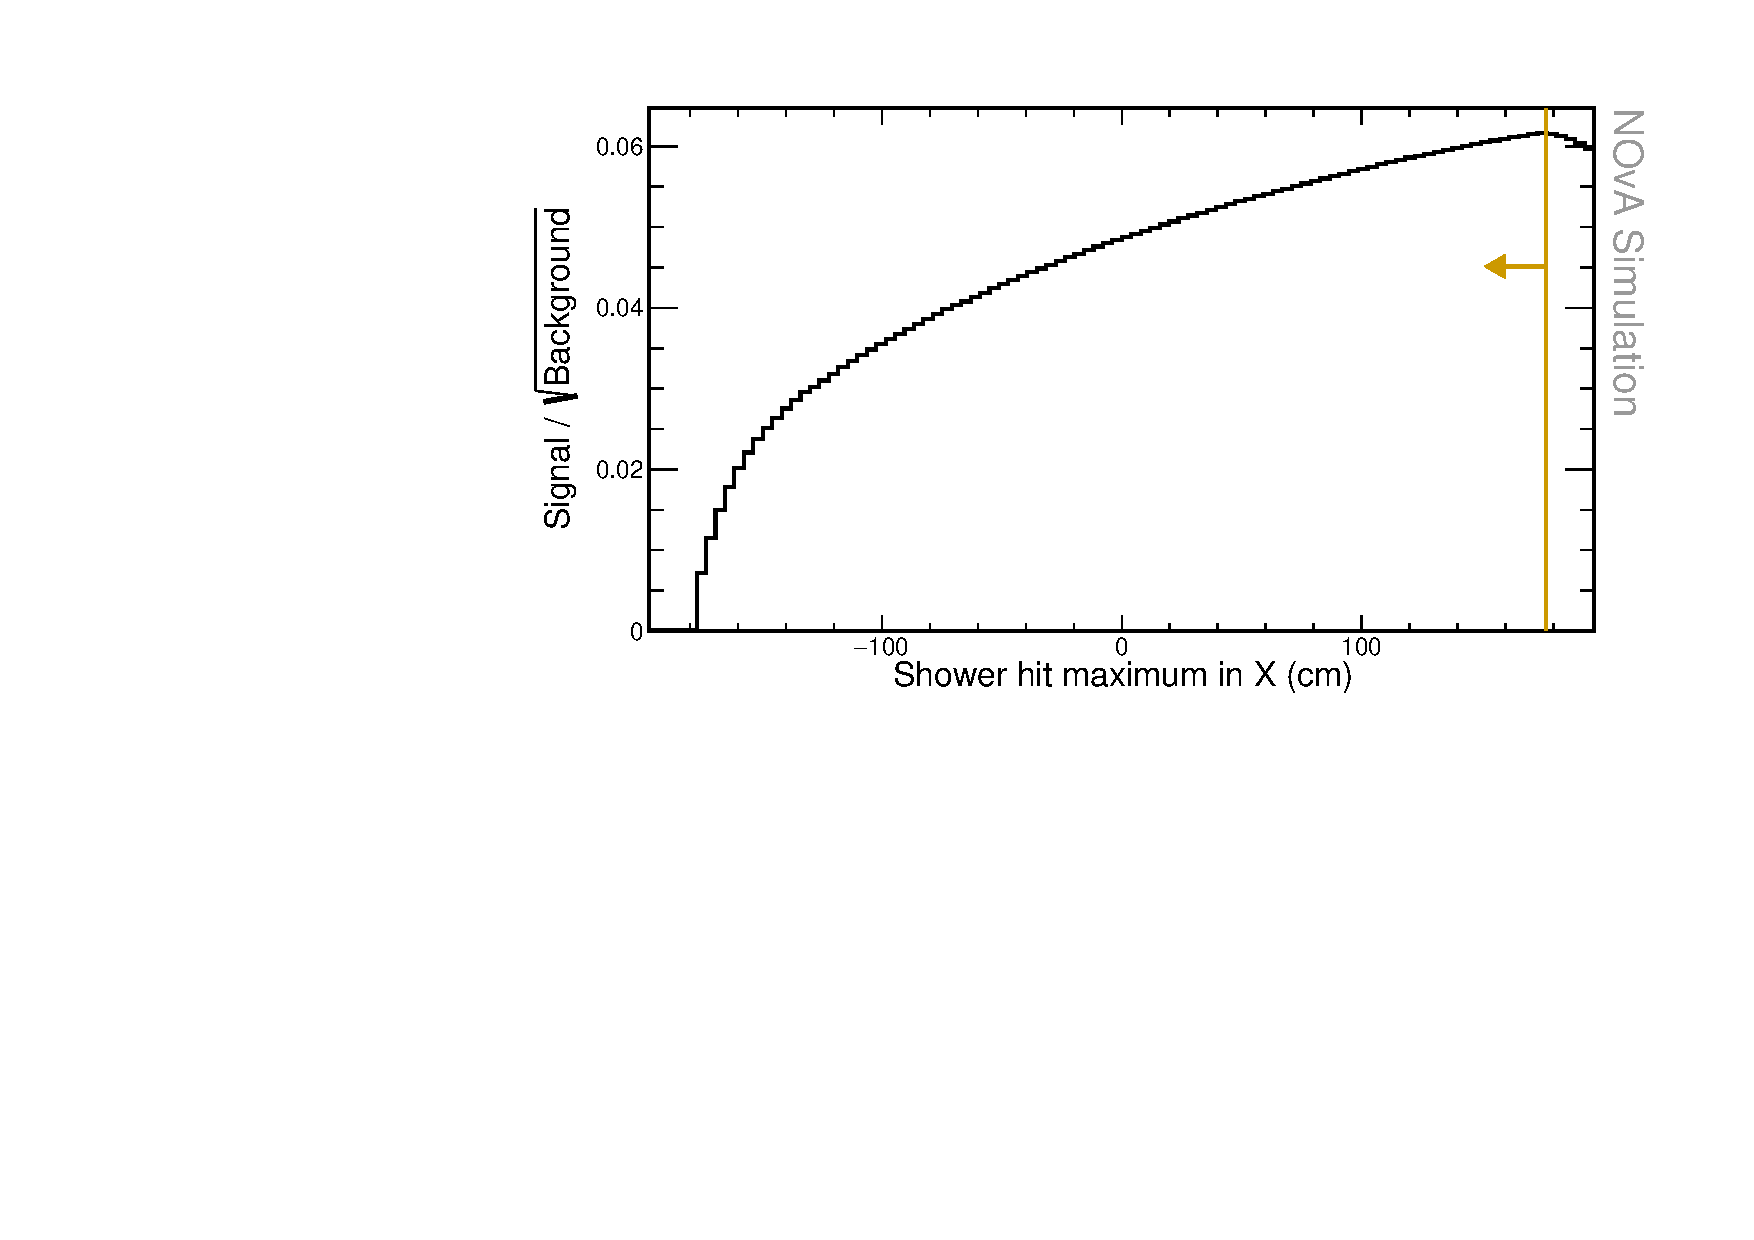
\includegraphics[width=.9\textwidth]{Plots/NuMMEventSelection/NuMM_N1Cut_maxXleft_FOMStats}
\caption{Relative comparison of signal, $\nu$-on-e background, and other background events for the minimum and maximum position of the reconstructed shower along the x axis. Pre-selection and fiducial cuts were applied to make these plots. Gold lines show the values of the containment cuts.}
\label{fig:NuMMContainmentCutMaxX}
\end{figure}

\begin{figure}[hbtp]
\centering
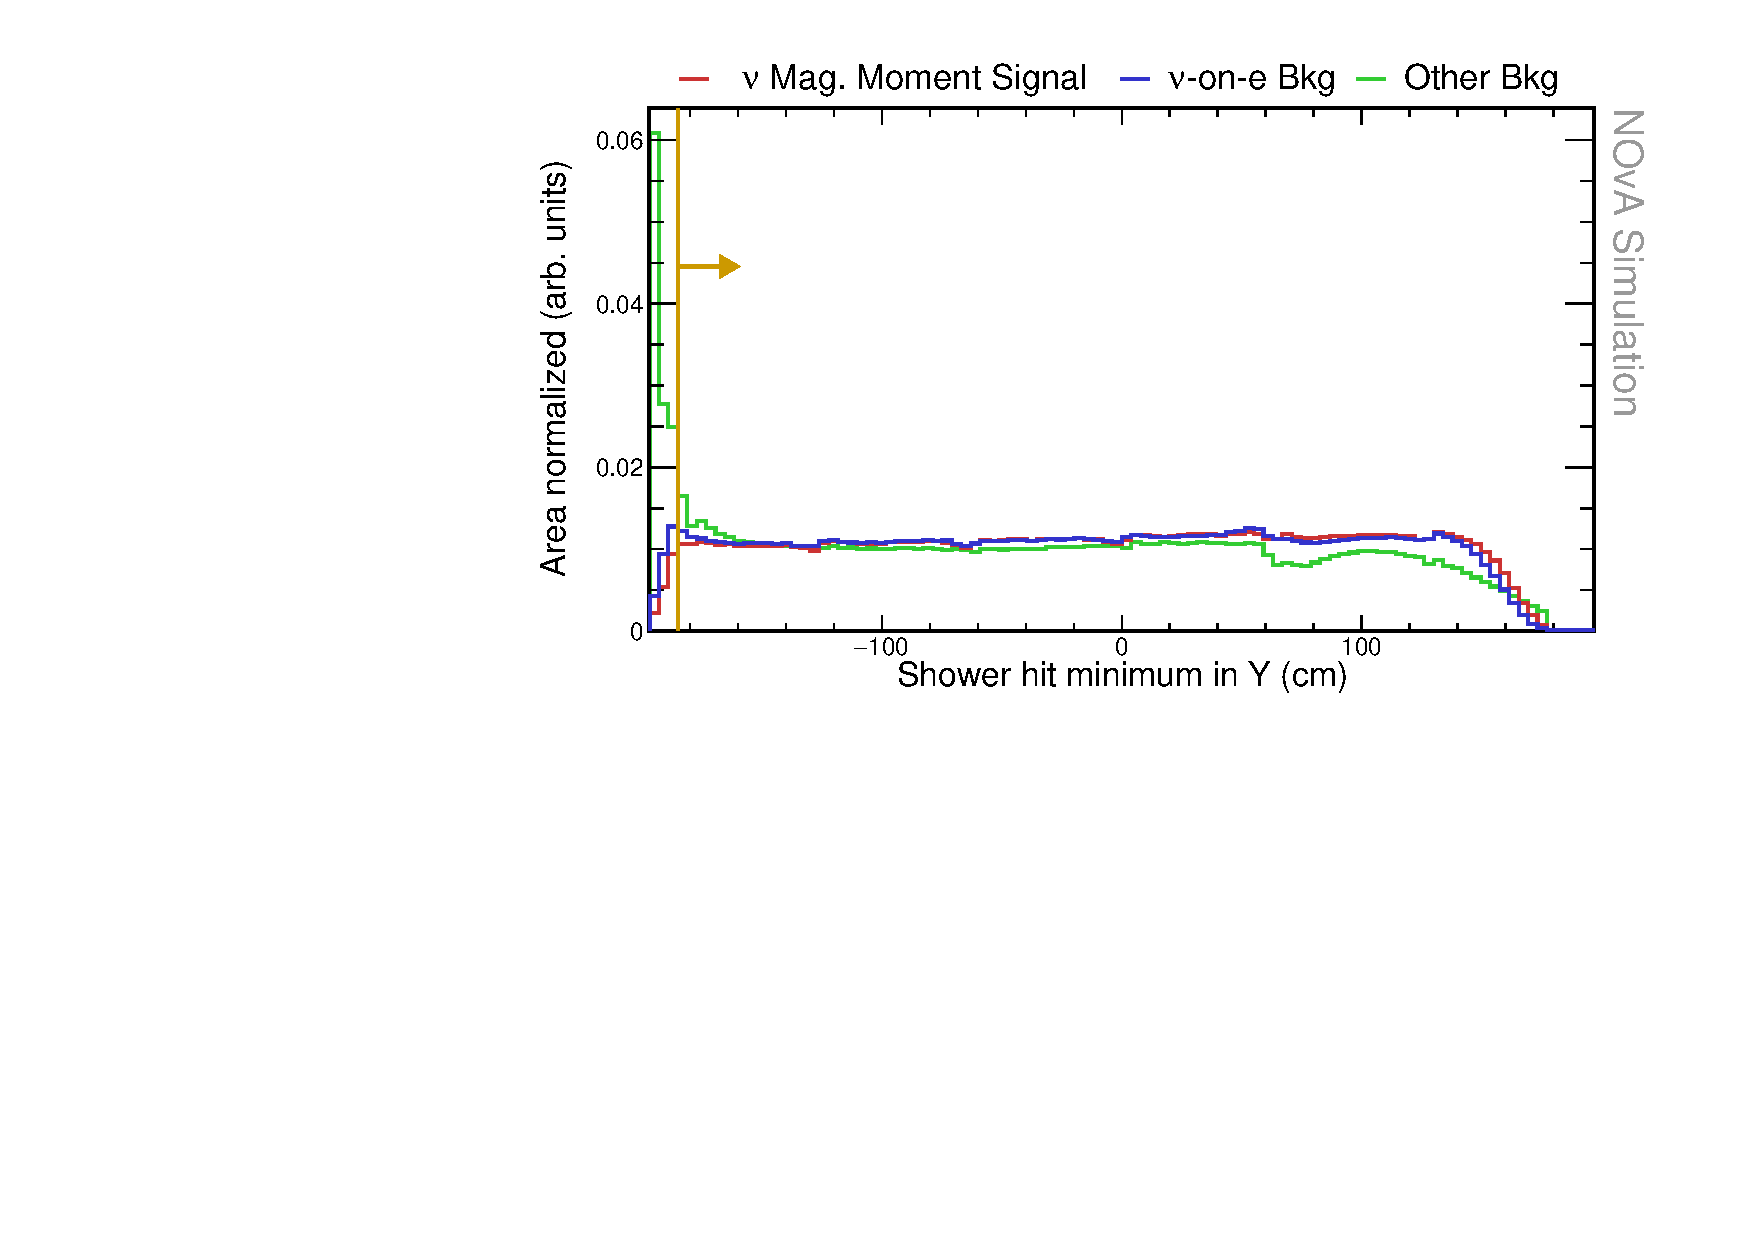
\includegraphics[width=.9\textwidth]{Plots/NuMMEventSelection/N1Cut_minY.pdf}
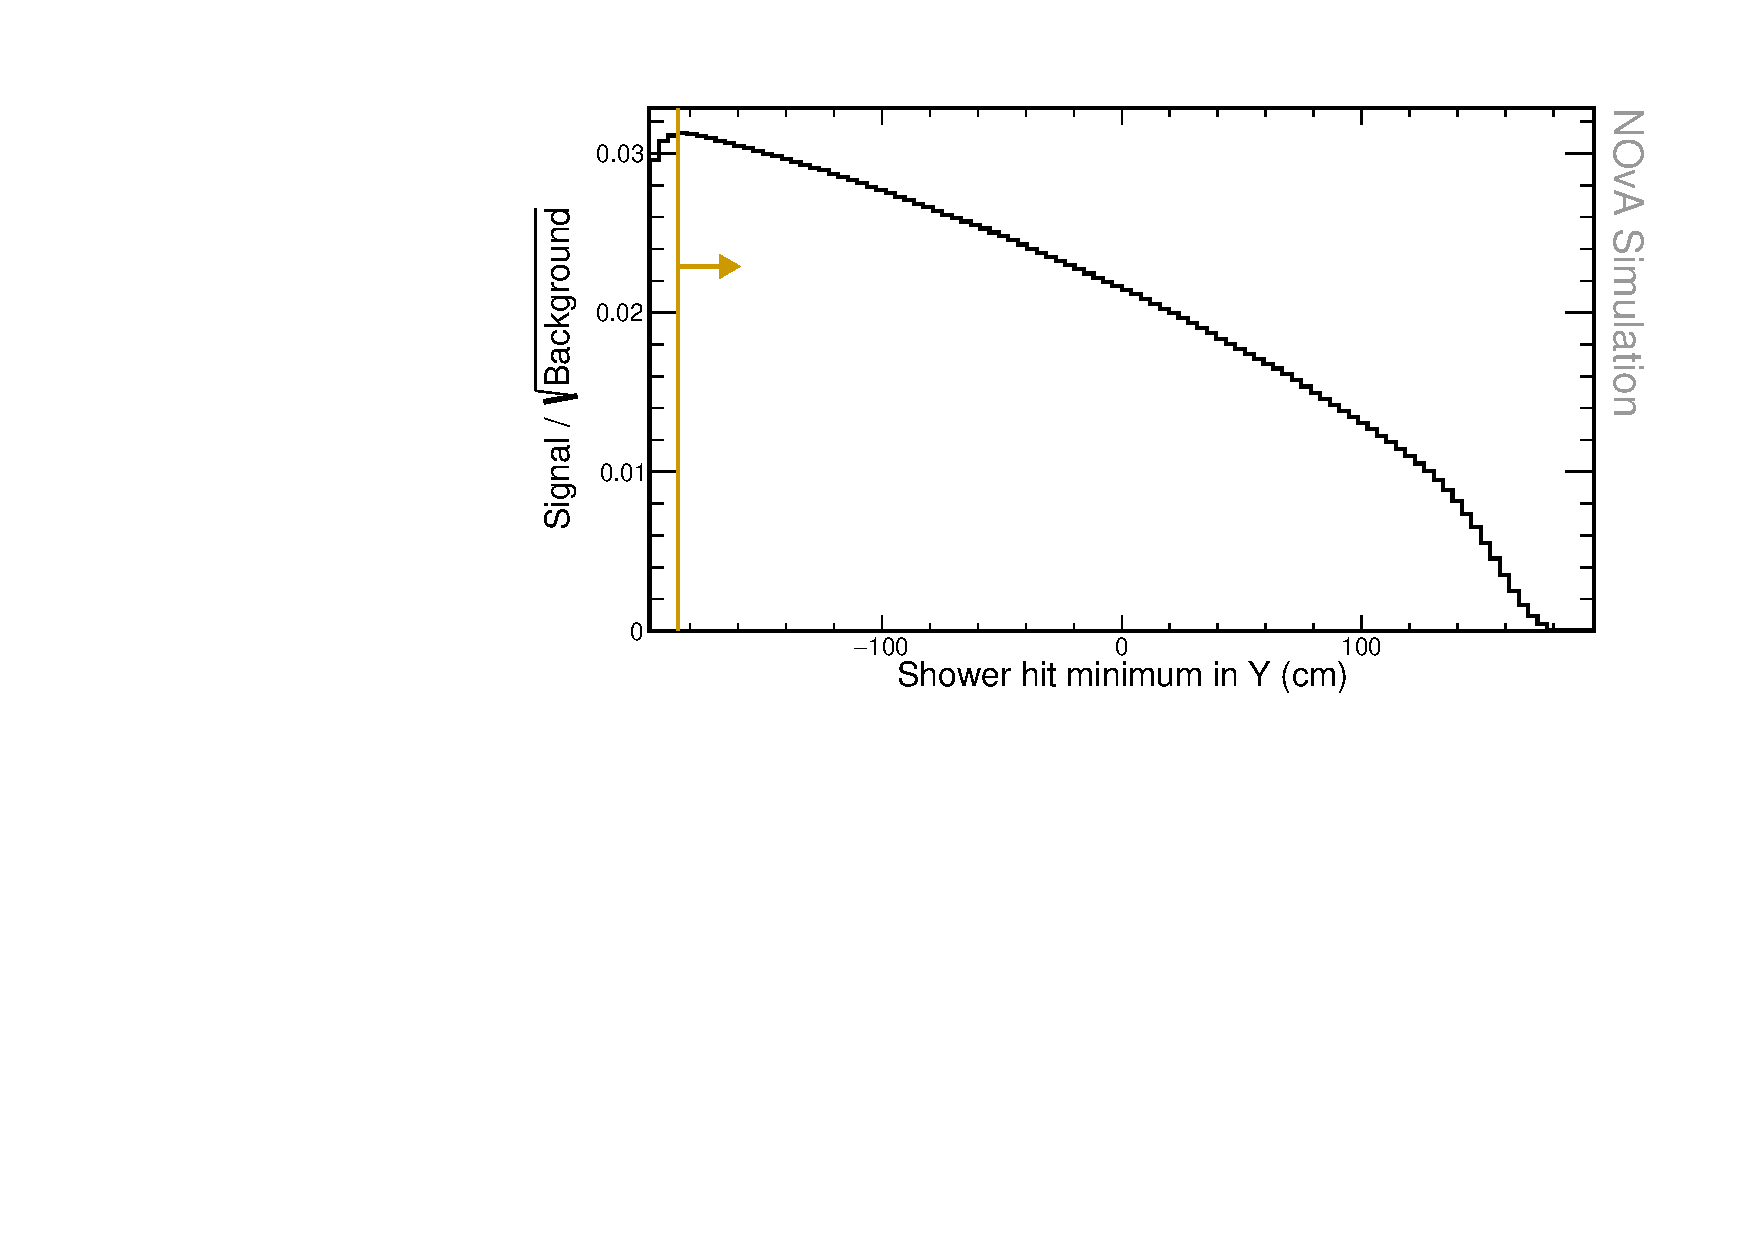
\includegraphics[width=.9\textwidth]{Plots/NuMMEventSelection/NuMM_N1Cut_minYright_FOMStats.pdf}
\caption{Relative comparison of signal, $\nu$-on-e background, and other background events for the minimum and maximum position of the reconstructed shower along the y axis. Pre-selection and fiducial cuts were applied to make these plots. Gold lines show the values of the containment cuts.}
\label{fig:NuMMContainmentCutMinY}
\end{figure}

\begin{figure}[hbtp]
\centering
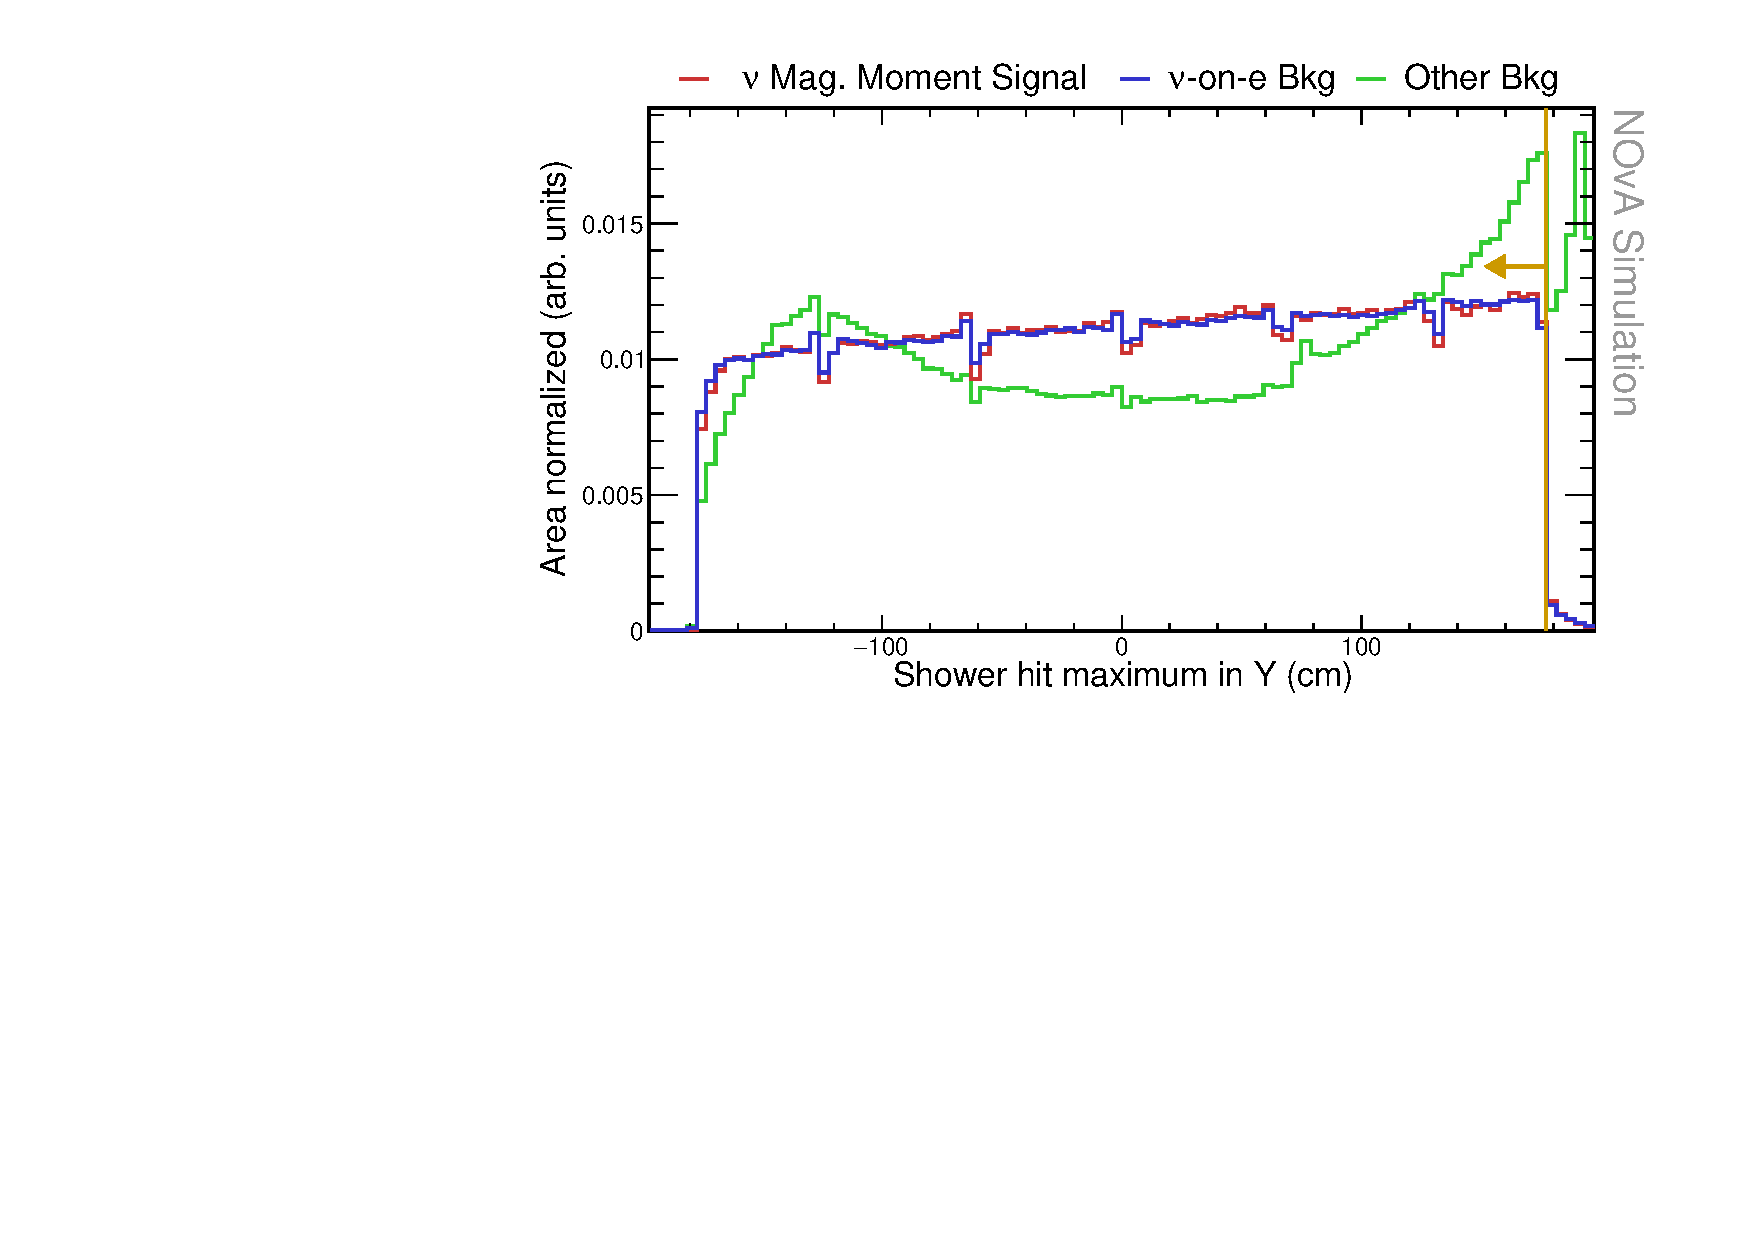
\includegraphics[width=.9\textwidth]{Plots/NuMMEventSelection/N1Cut_maxY.pdf}
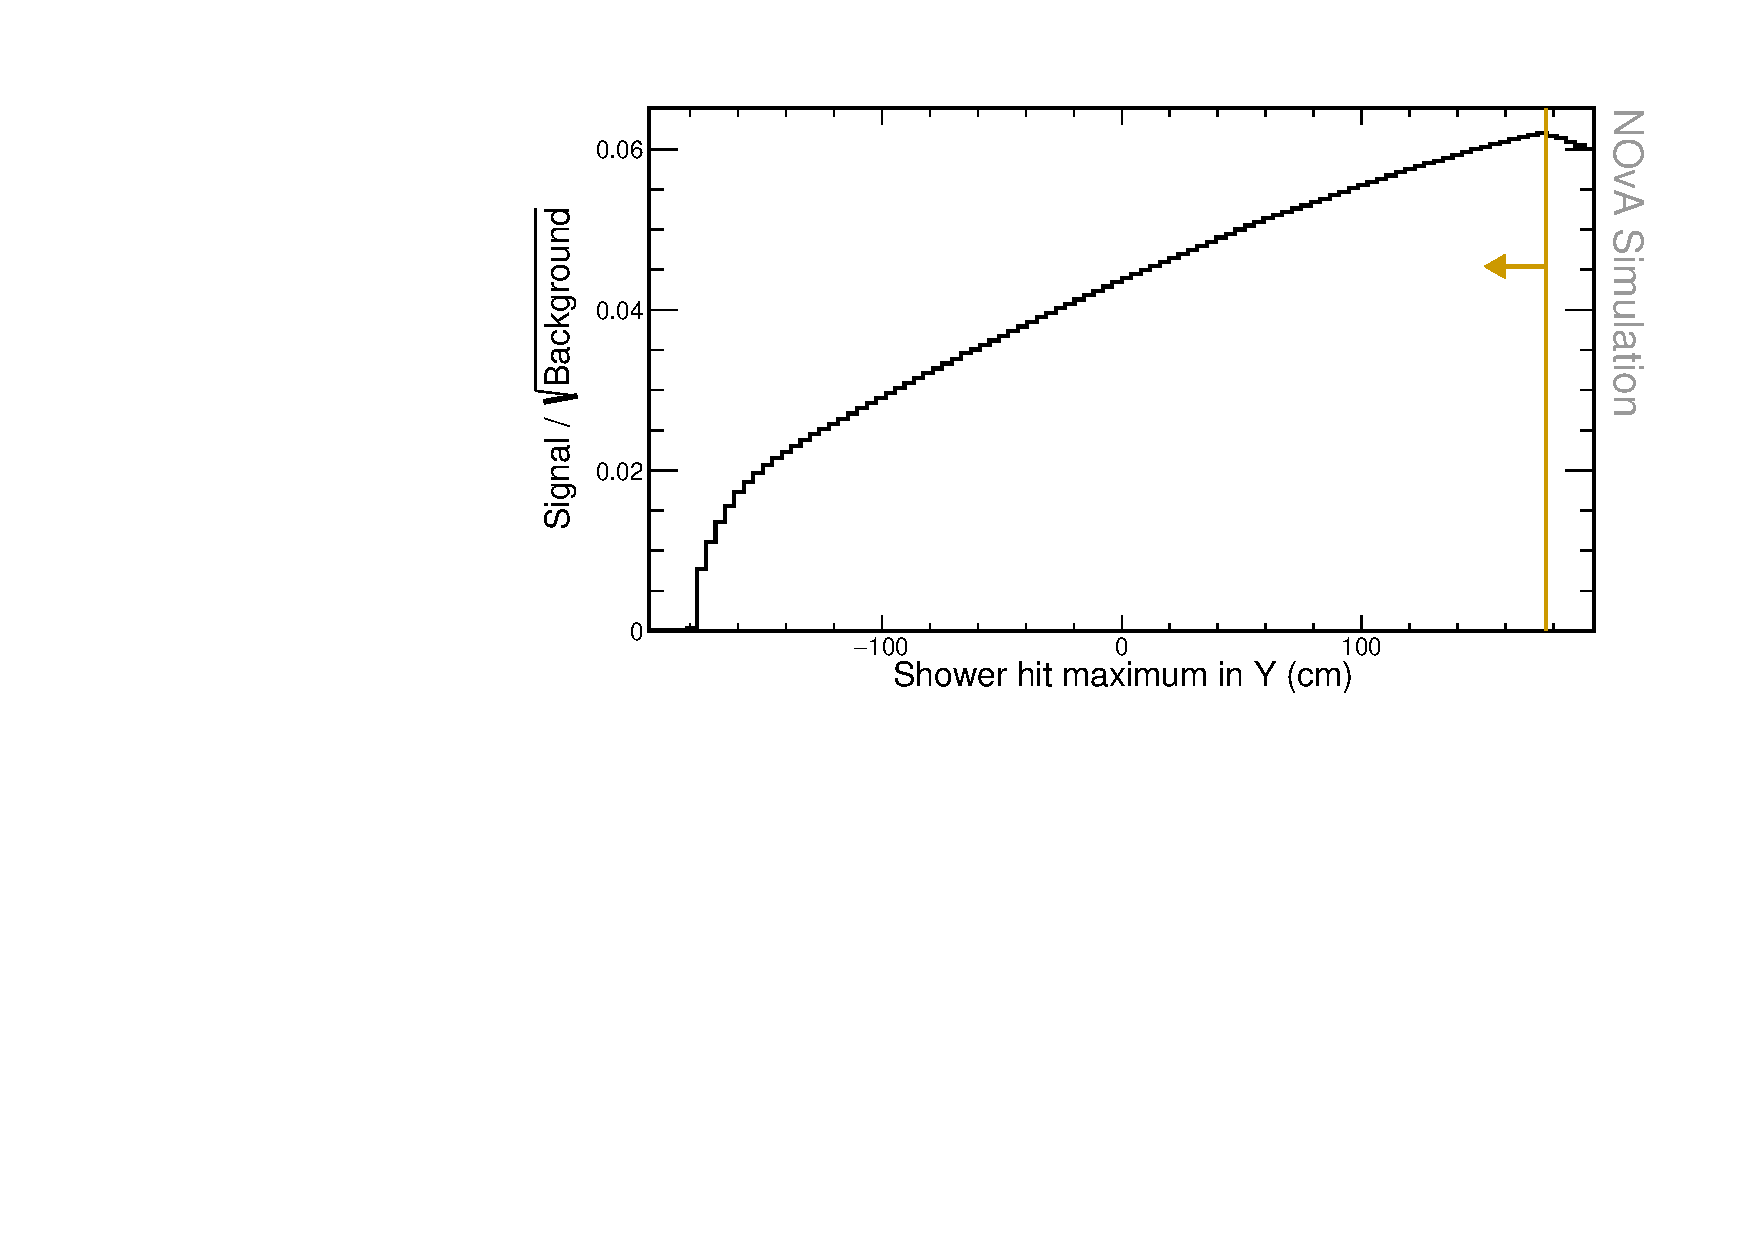
\includegraphics[width=.9\textwidth]{Plots/NuMMEventSelection/NuMM_N1Cut_maxYleft_FOMStats}
\caption{Relative comparison of signal, $\nu$-on-e background, and other background events for the minimum and maximum position of the reconstructed shower along the y axis. Pre-selection and fiducial cuts were applied to make these plots. Gold lines show the values of the containment cuts.}
\label{fig:NuMMContainmentCutMaxY}
\end{figure}

\begin{figure}[hbtp]
\centering
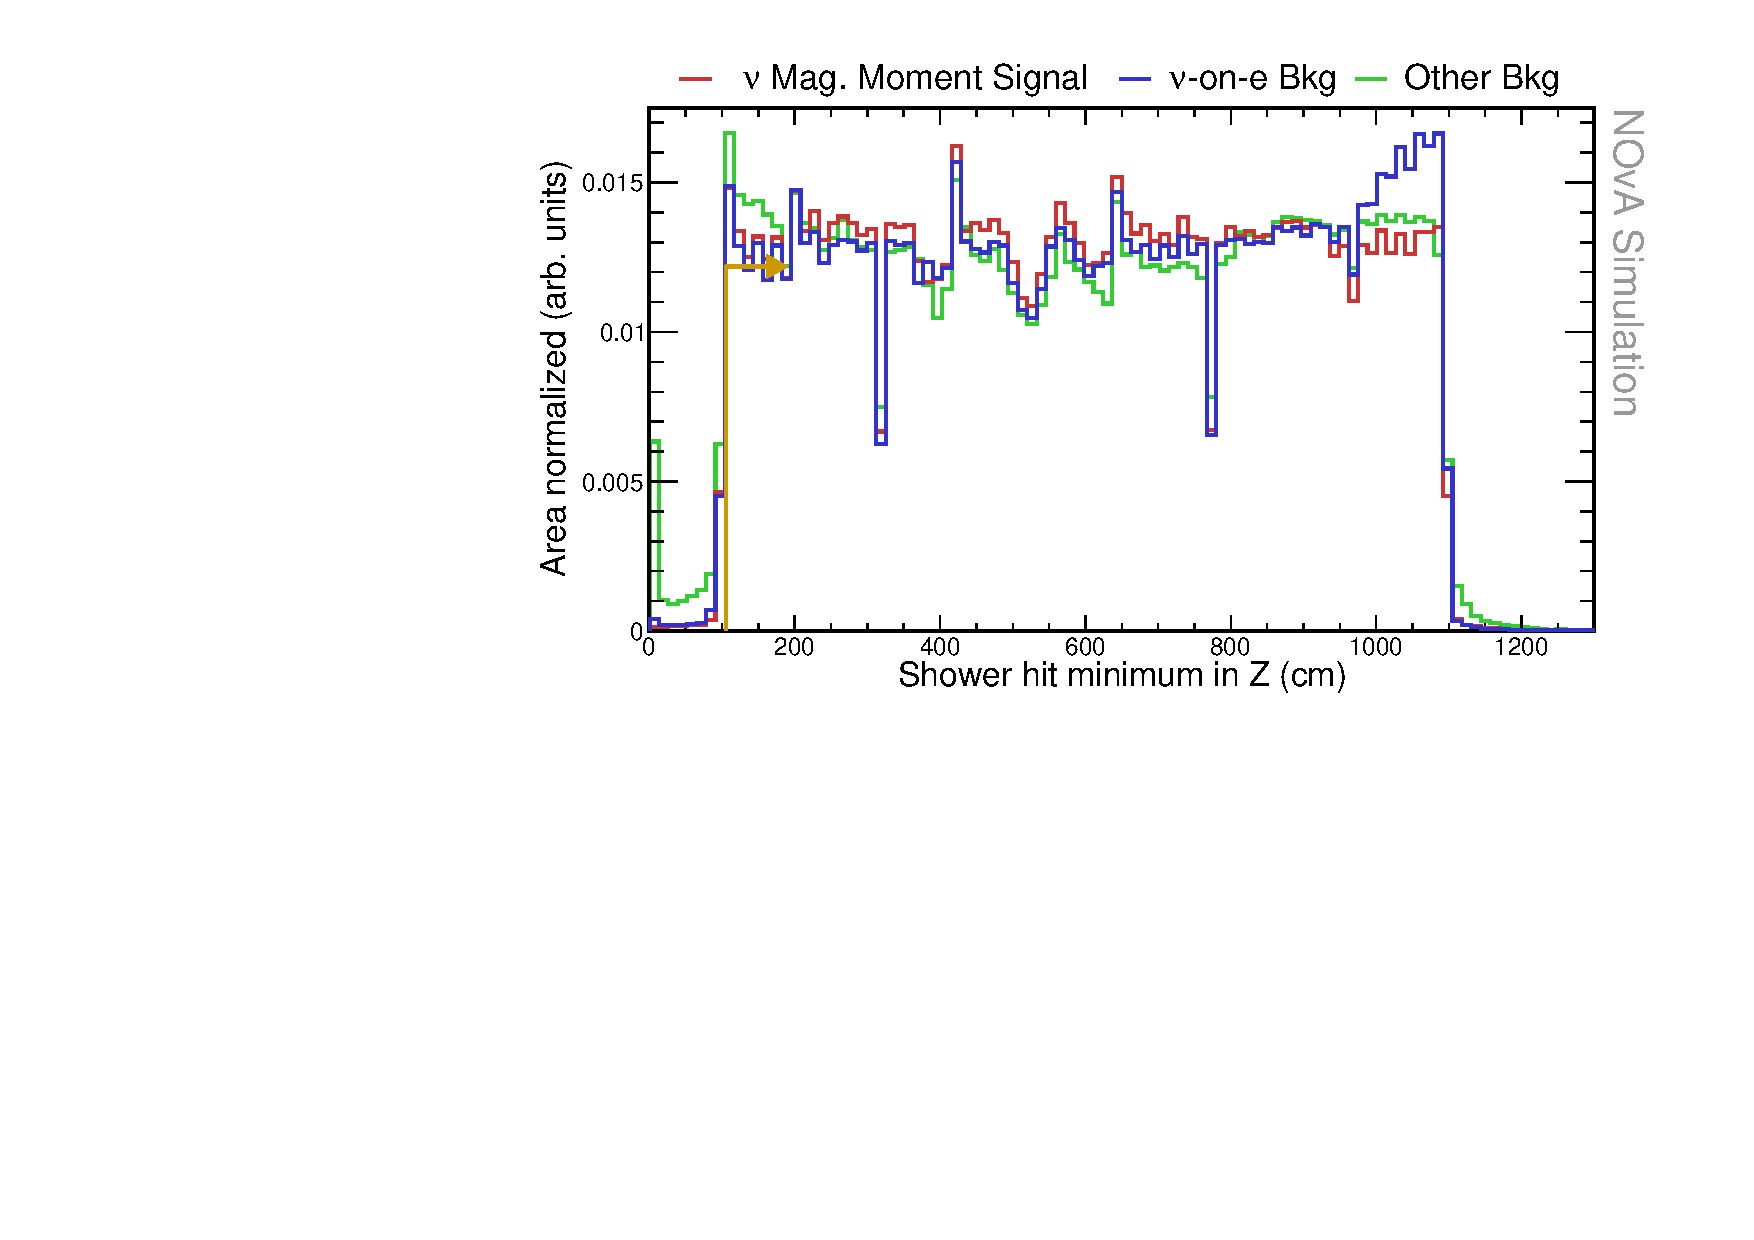
\includegraphics[width=.9\textwidth]{Plots/NuMMEventSelection/N1Cut_minZ.pdf}
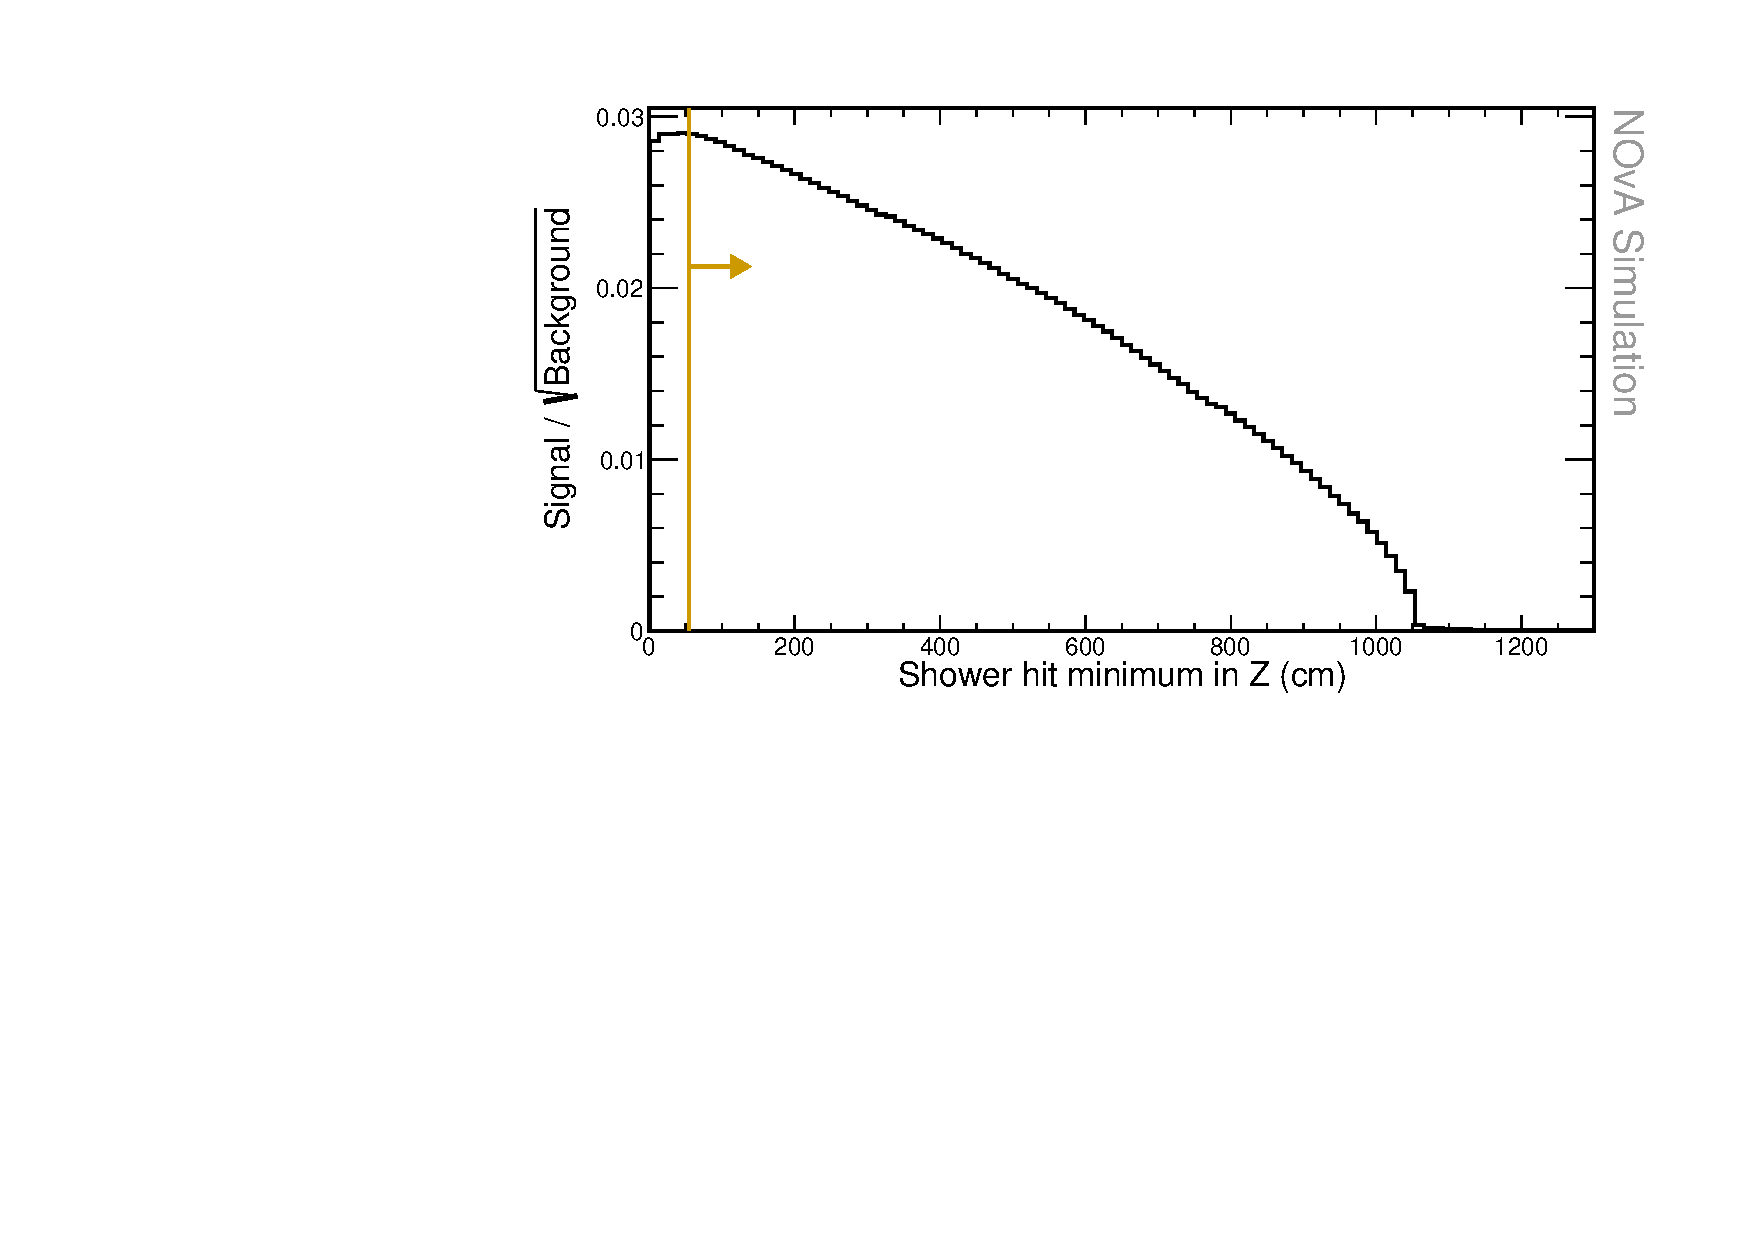
\includegraphics[width=.9\textwidth]{Plots/NuMMEventSelection/NuMM_N1Cut_minZright_FOMStats.pdf}
\caption{Relative comparison of signal, $\nu$-on-e background, and other background events for the minimum and maximum position of the reconstructed shower along the z axis. Pre-selection and fiducial cuts were applied to make these plots. Gold lines show the values of the containment cuts.}
\label{fig:NuMMContainmentCutMinZ}
\end{figure}

\begin{figure}[hbtp]
\centering
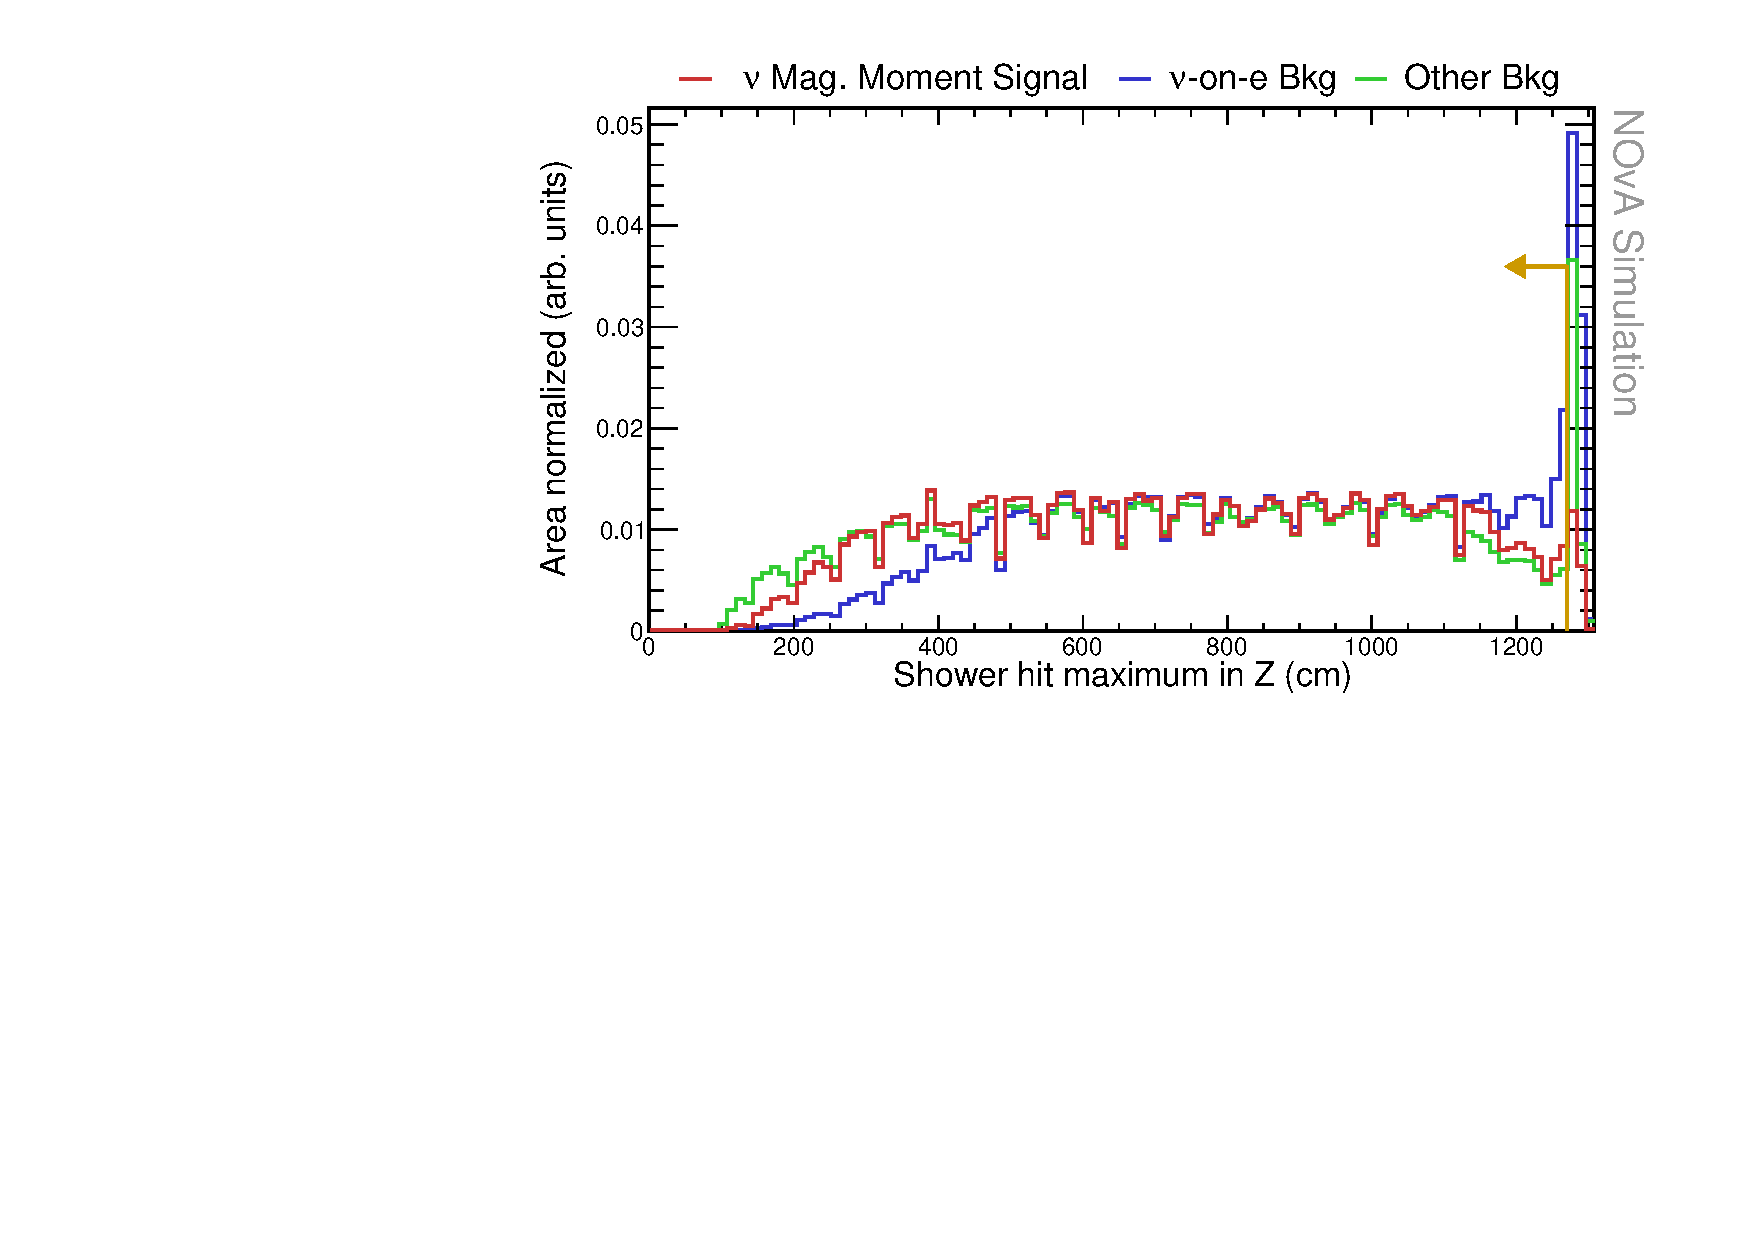
\includegraphics[width=.9\textwidth]{Plots/NuMMEventSelection/N1Cut_maxZ.pdf}
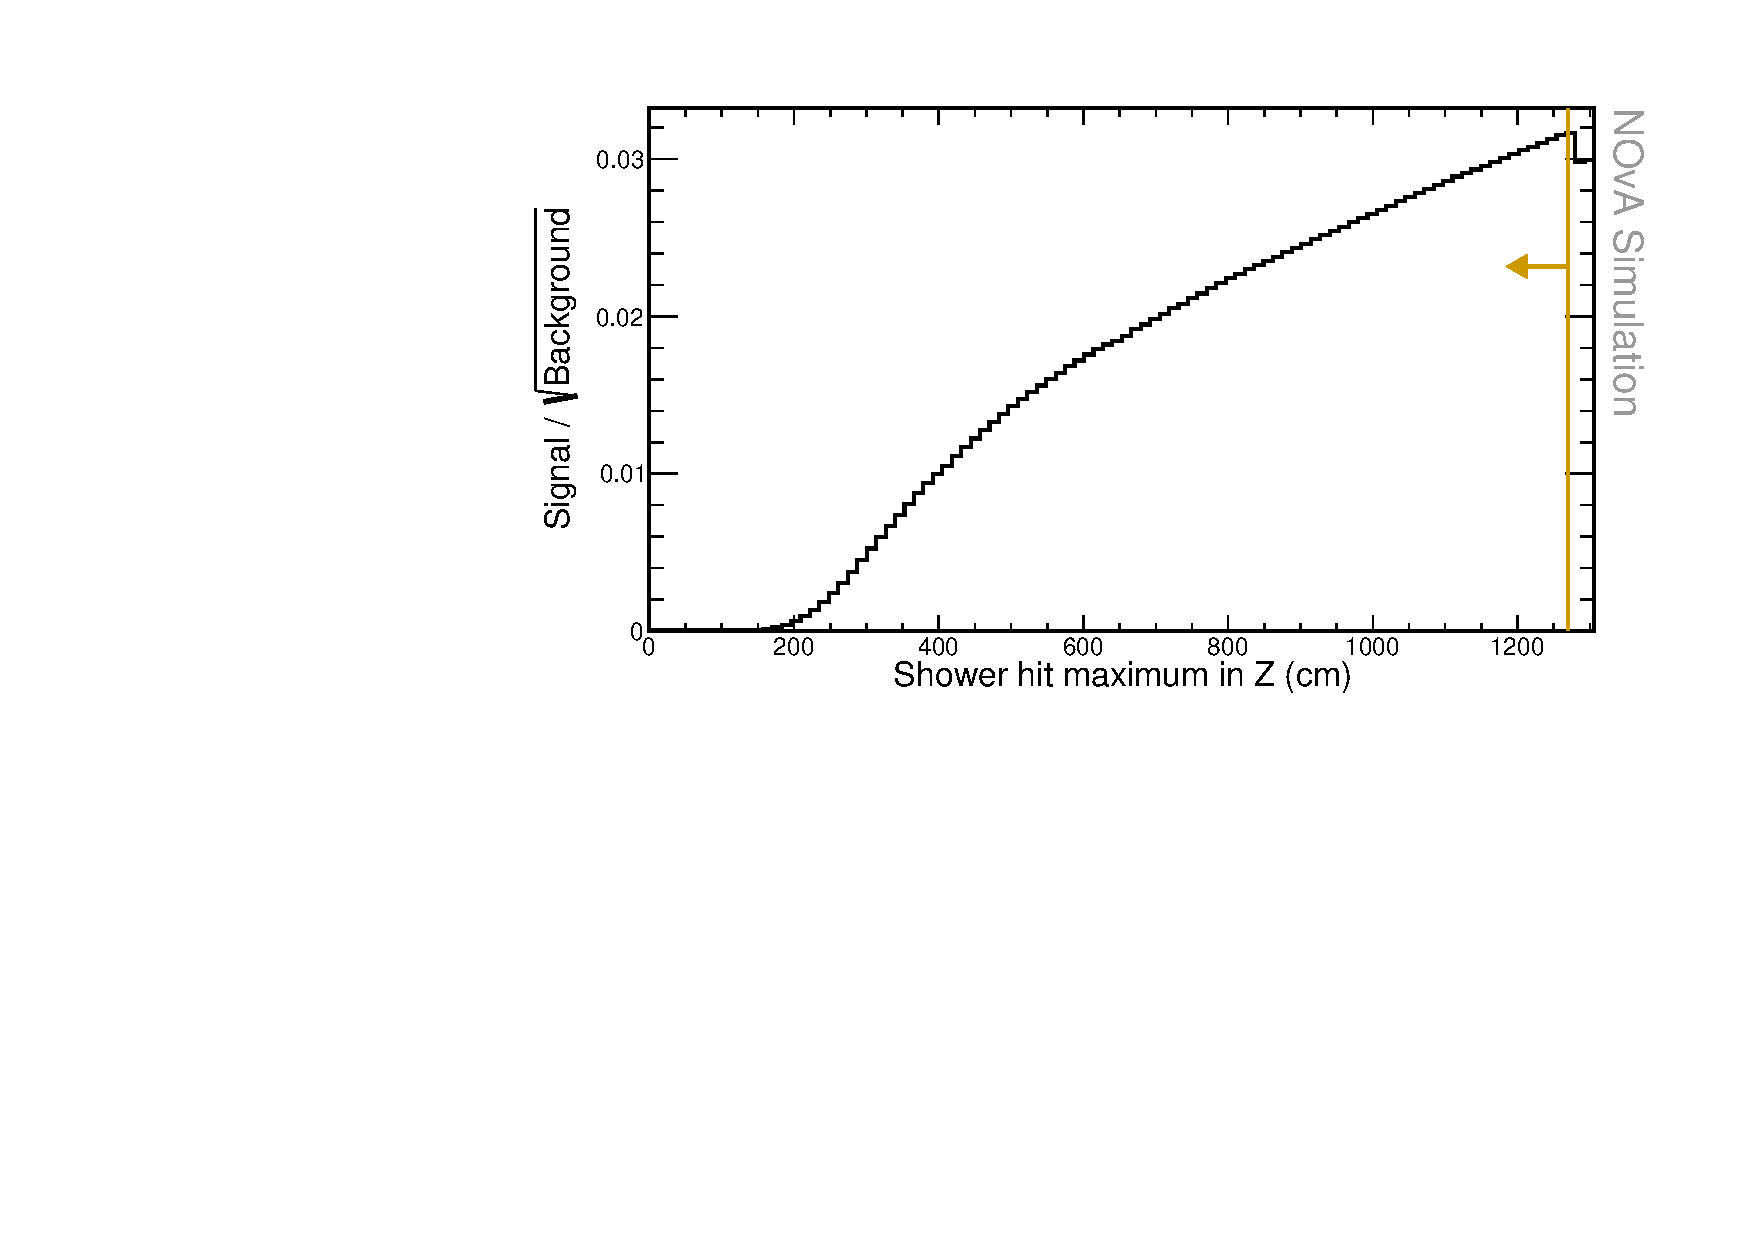
\includegraphics[width=.9\textwidth]{Plots/NuMMEventSelection/NuMM_N1Cut_maxZleft_FOMStats}
\caption{Relative comparison of signal, $\nu$-on-e background, and other background events for the minimum and maximum position of the reconstructed shower along the z axis. Pre-selection and fiducial cuts were applied to make these plots. Gold lines show the values of the containment cuts.}
\label{fig:NuMMContainmentCutMaxZ}
\end{figure}

\begin{table}[!hb]
\centering
\caption[Event selection cutflow table for the reconstruction quality cut]{Event selection cutflow table for the reconstruction quality cuts showing the number of events and the relative efficiency of each cut for each signal sample. The relative efficiency is calculated as number of events remaining after applying the corresponding cut divided by number of event for all the previous cuts. All the cuts are listed in sequence as they are applied.}
\begin{tabular}{|l|cc|cc|cc|}\hline
\multicolumn{1}{|c|}{} & \multicolumn{2}{c|}{\textbf{Signal}} & \multicolumn{2}{c|}{\textbf{$\nu$-on-e bkg}} & \multicolumn{2}{c|}{\textbf{Other bkg}} \\
\multicolumn{1}{|c|}{\multirow{-2}{*}{\textbf{Selection}}} & \textbf{$N_{evt}$} & \textbf{$\epsilon_{rel}\left(\%\right)$} & \textbf{$N_{evt}$} & \textbf{$\epsilon_{rel}\left(\%\right)$}  & \textbf{$N_{evt}$} & \textbf{$\epsilon_{rel}\left(\%\right)$}\\\hline
\textbf{Basic selection} & 48.27 & 100 & 2.03$\times 10^3$ & 100 & 5.98$\times 10^6$ & 100\\
\textbf{Fiducial} & 45.51 & 94.27 & 1.89$\times 10^3$ & 93.36 & 2.89$\times 10^6$ & 48.22\\
\textbf{Containment} & 42.01 & 92.31 & 1.62$\times 10^3$ & 85.42 & 7.22$\times 10^5$ & 25.04\\\hline
\end{tabular}
\label{tab:CutflowTableFiducialContainmnet}
\end{table}

\subsection{Event Selection Optimization}
\note{This is where I started the TMVA}

\subsubsection*{Single Shower Requirement}

To selection events with a single particle we require that the fraction of energy contained in the most energetic shower is $>0.8$, that the summed energy of all cells (above threshold and within $\pm8$ planes from the vertex) outside of the most energetic shower is $<0.02\ \unit{GeV}$, and that the distance between the vertex and the start of the primary shower is $<20\ \unit{cm}$.

\begin{figure}[hbtp]
\centering
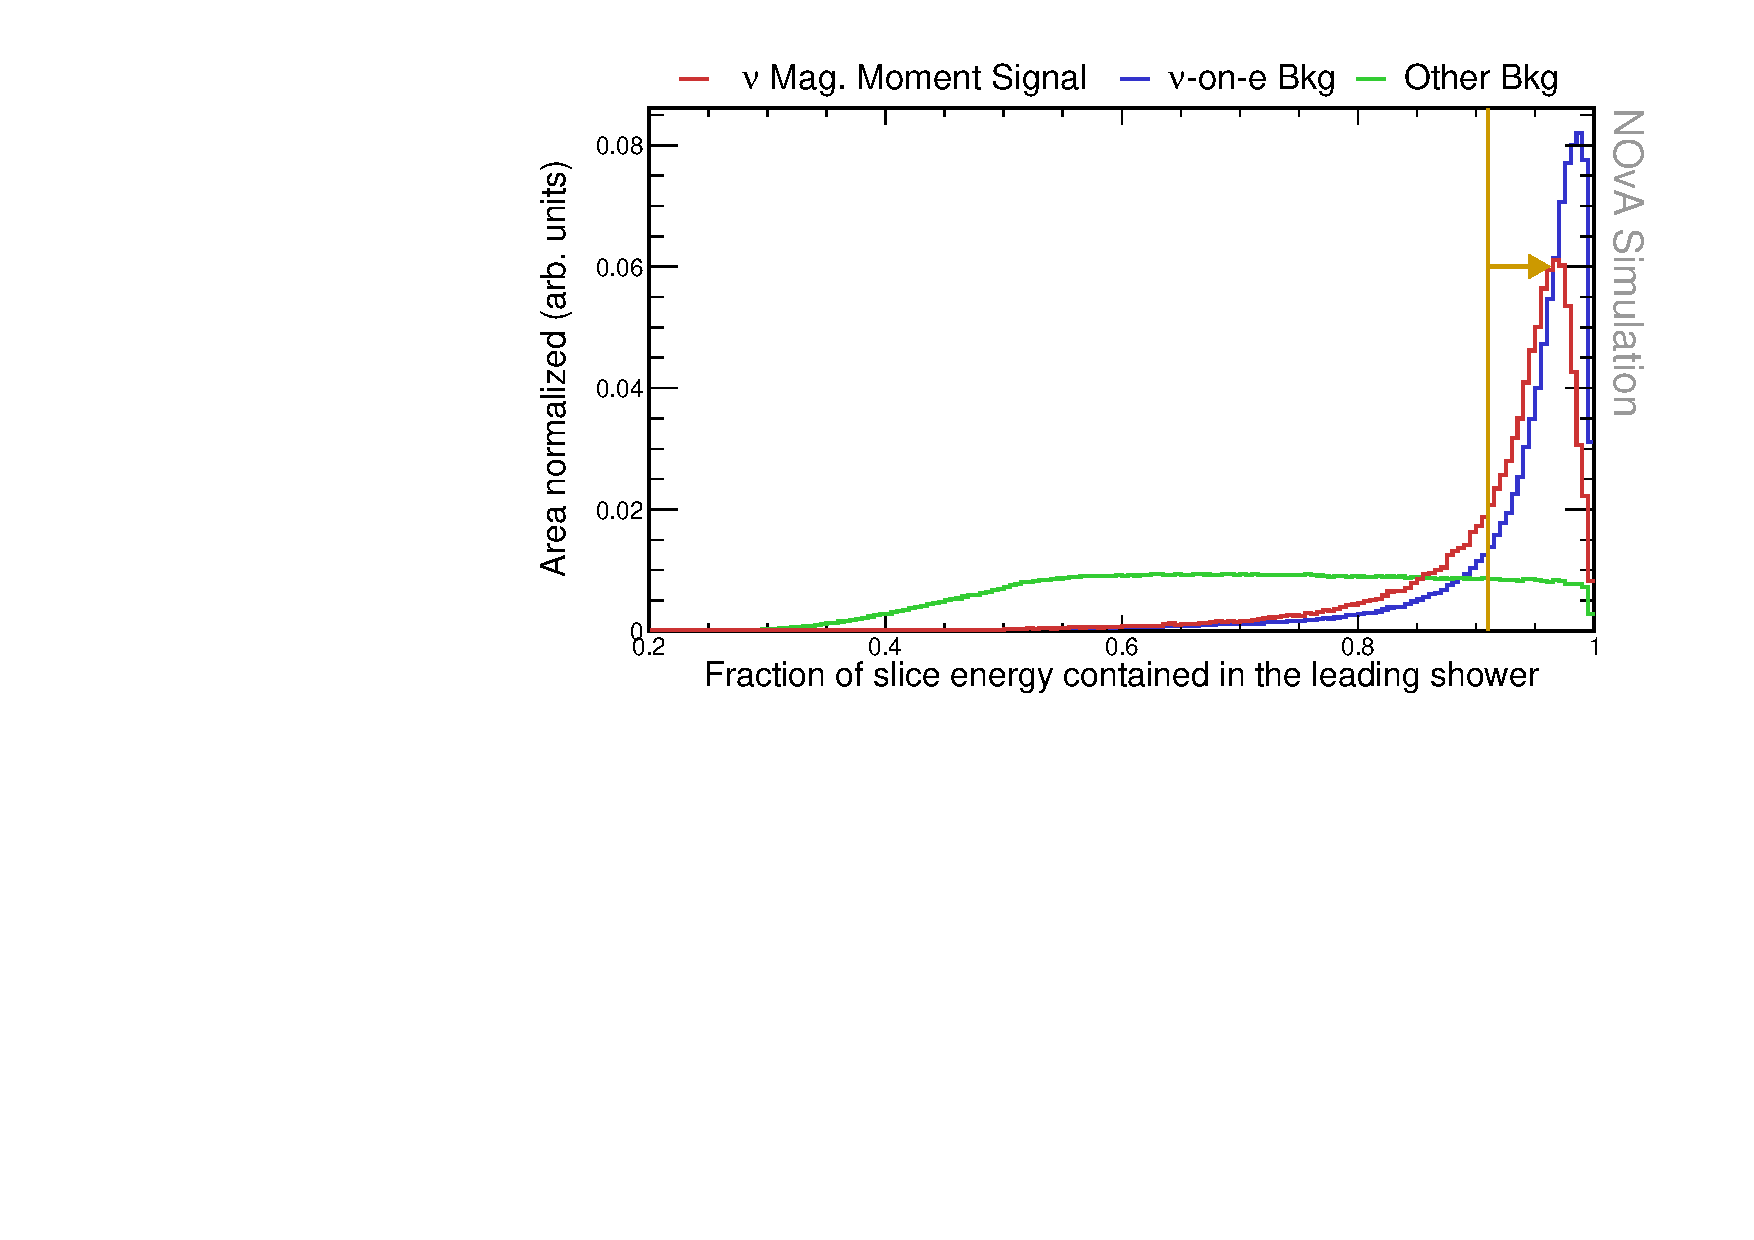
\includegraphics[width=.9\textwidth]{Plots/NuMMEventSelection/N1Cut_shwEFracPre.pdf}
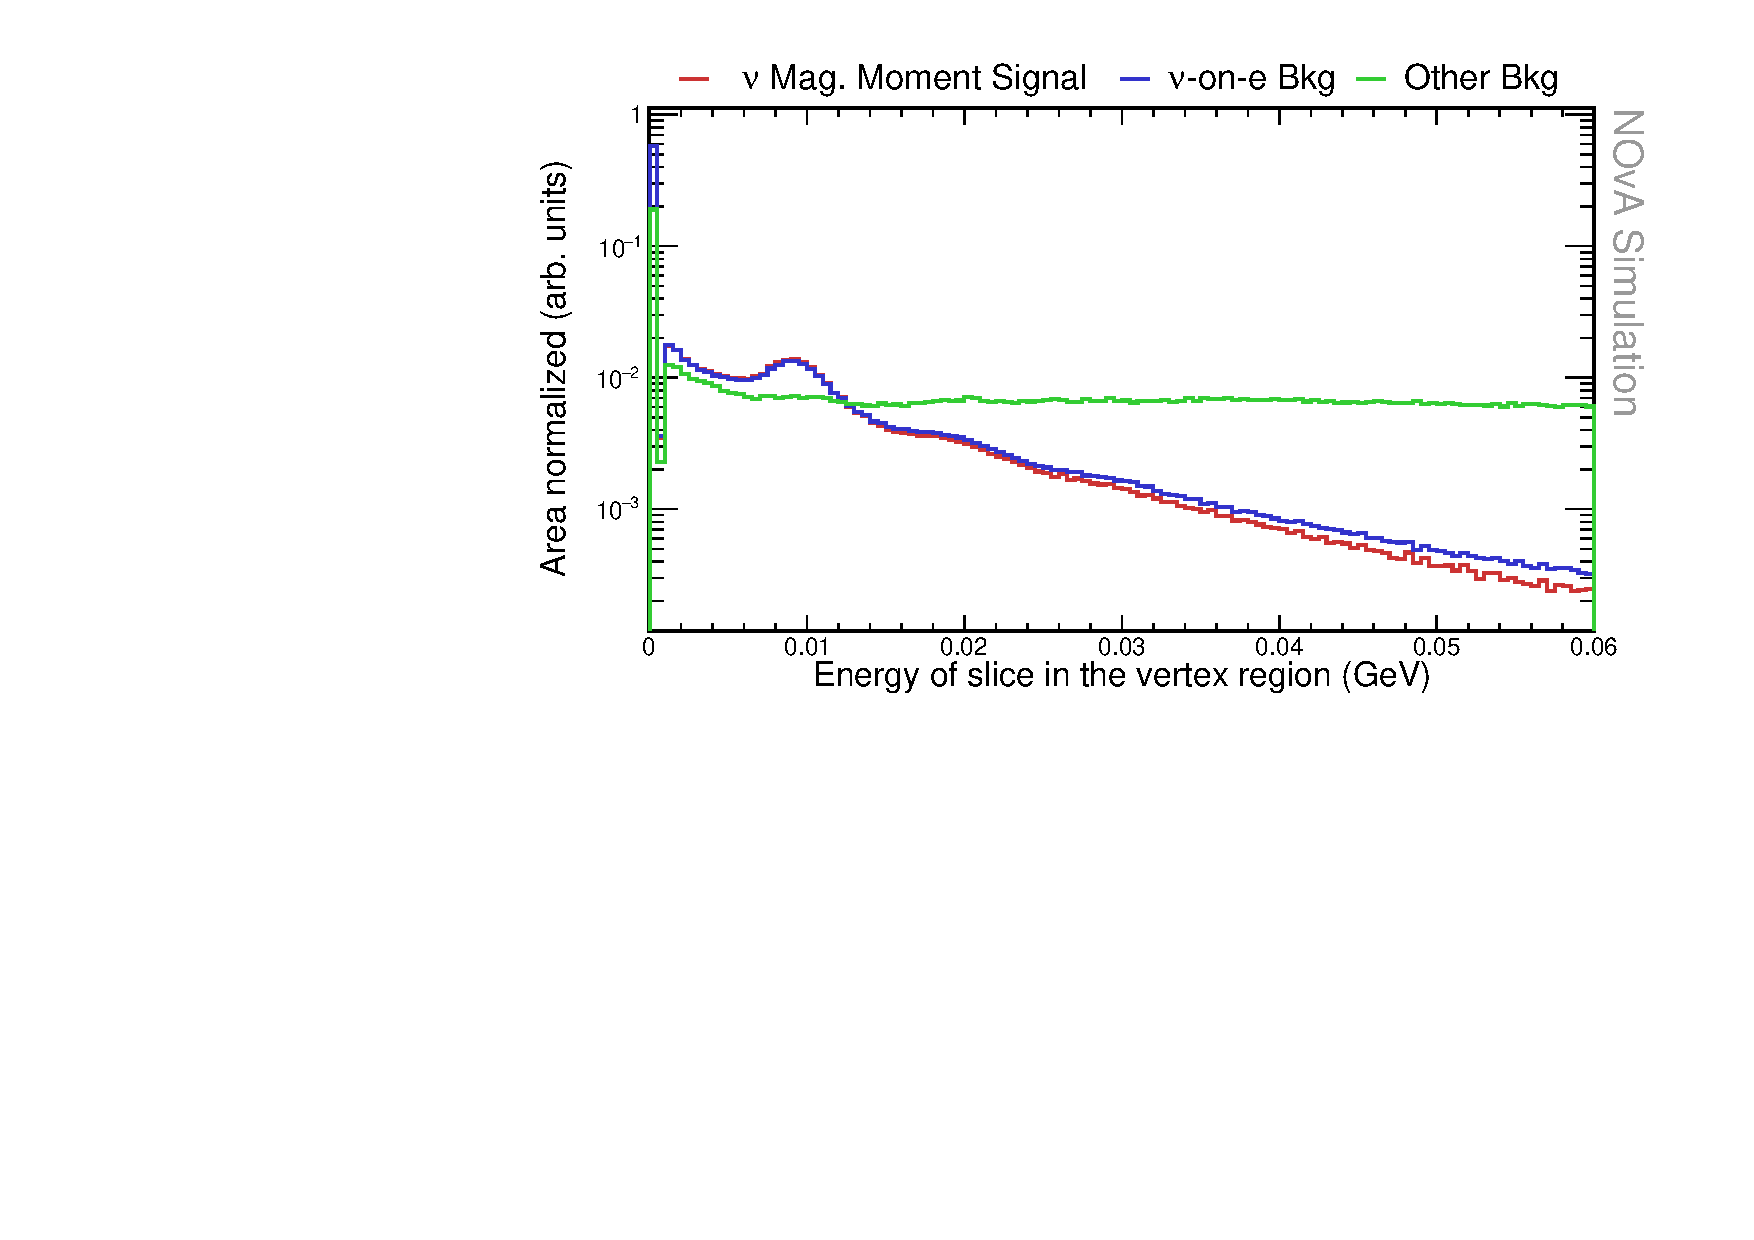
\includegraphics[width=.9\textwidth]{Plots/NuMMEventSelection/LogY_N1Cut_vtxEPre.pdf}
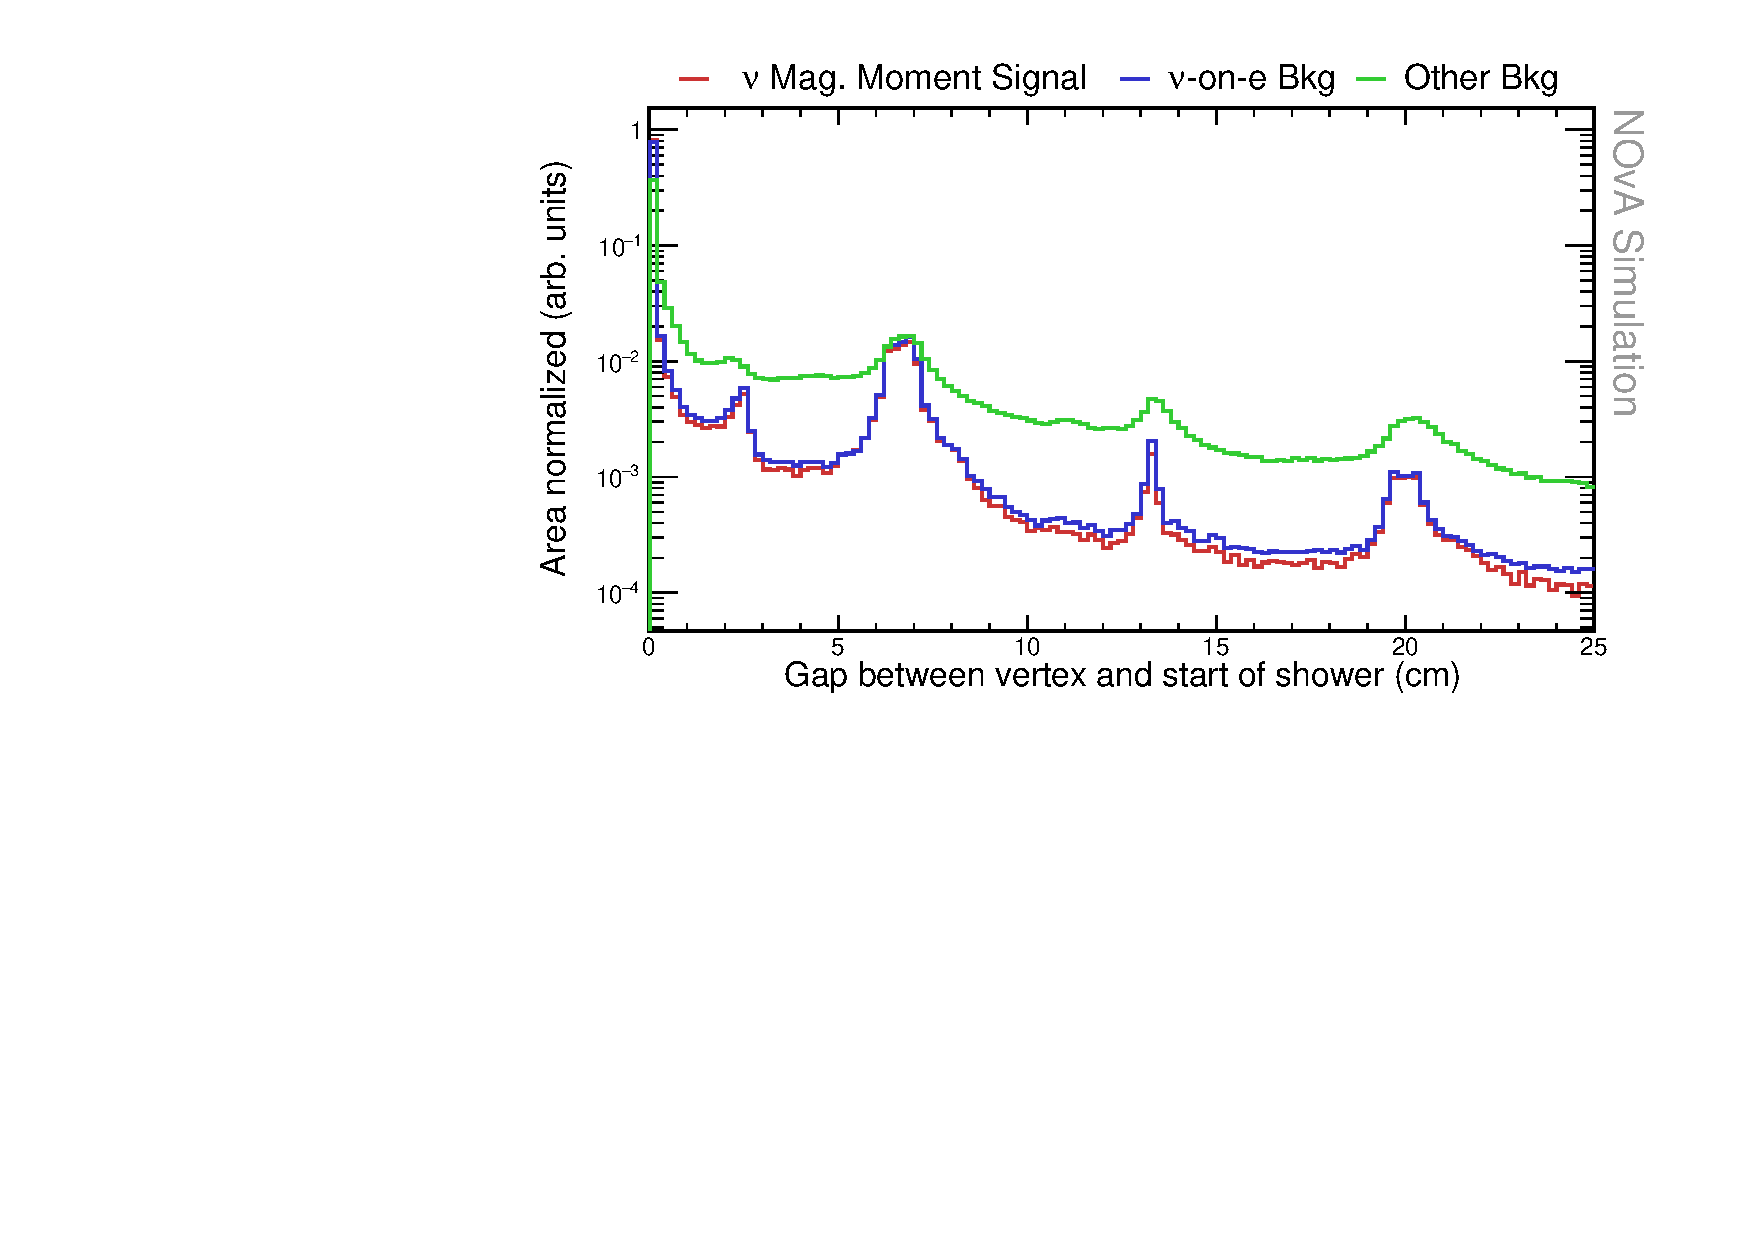
\includegraphics[width=.9\textwidth]{Plots/NuMMEventSelection/LogY_N1Cut_gapPre.pdf}
\caption{TMVA variables before the TMVA results. Relative comparison of signal, $\nu$-on-e background, and other background events for the reconstructed vertex. Every previous cut was applied to make these plots, including the ShwECont for the middle and the bottom plot and the VtxE cut for the bottom plot. Gold lines show the cut values that create the fiducial volume.}
\label{fig:SingleShowerCutsOld}
\end{figure}

\begin{figure}[hbtp]
\centering
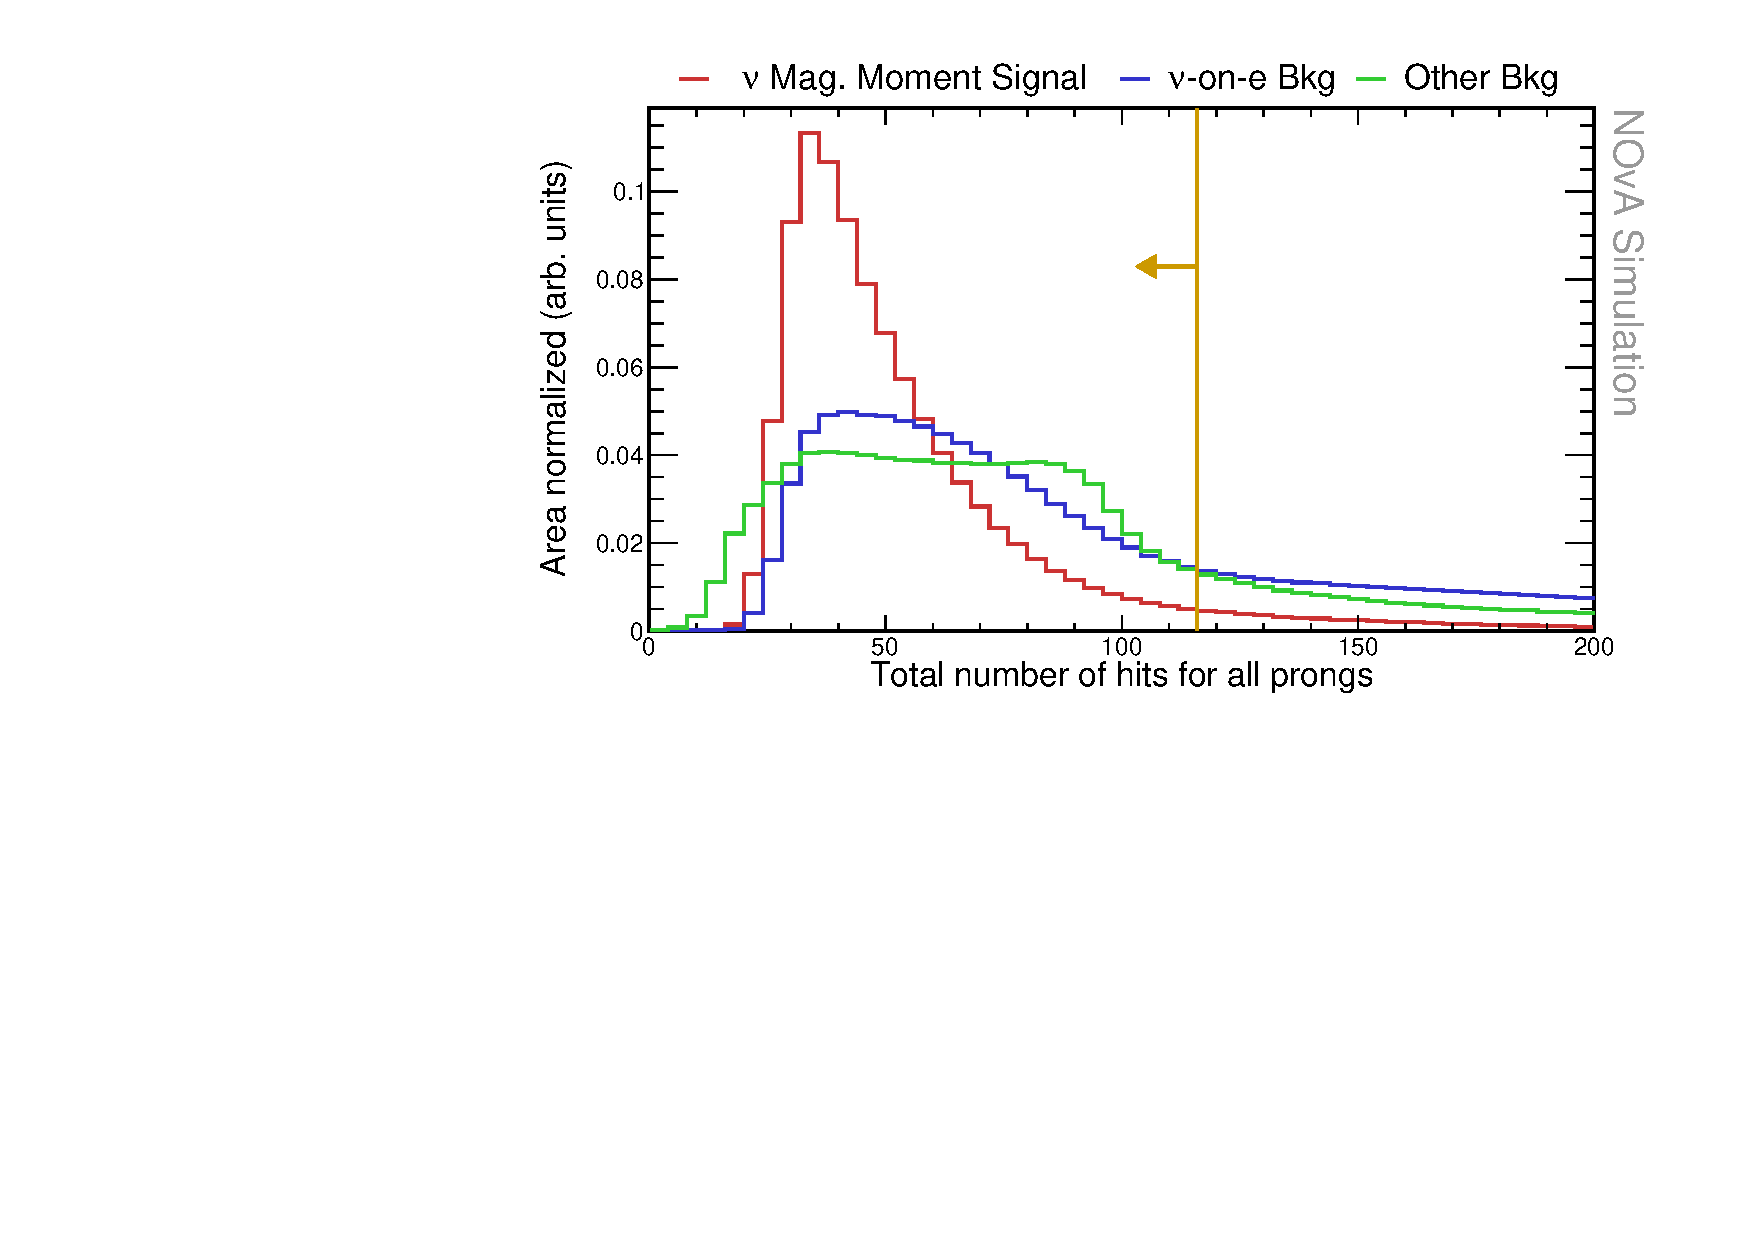
\includegraphics[width=.9\textwidth]{Plots/NuMMEventSelection/N1Cut_NHitsPre.pdf}
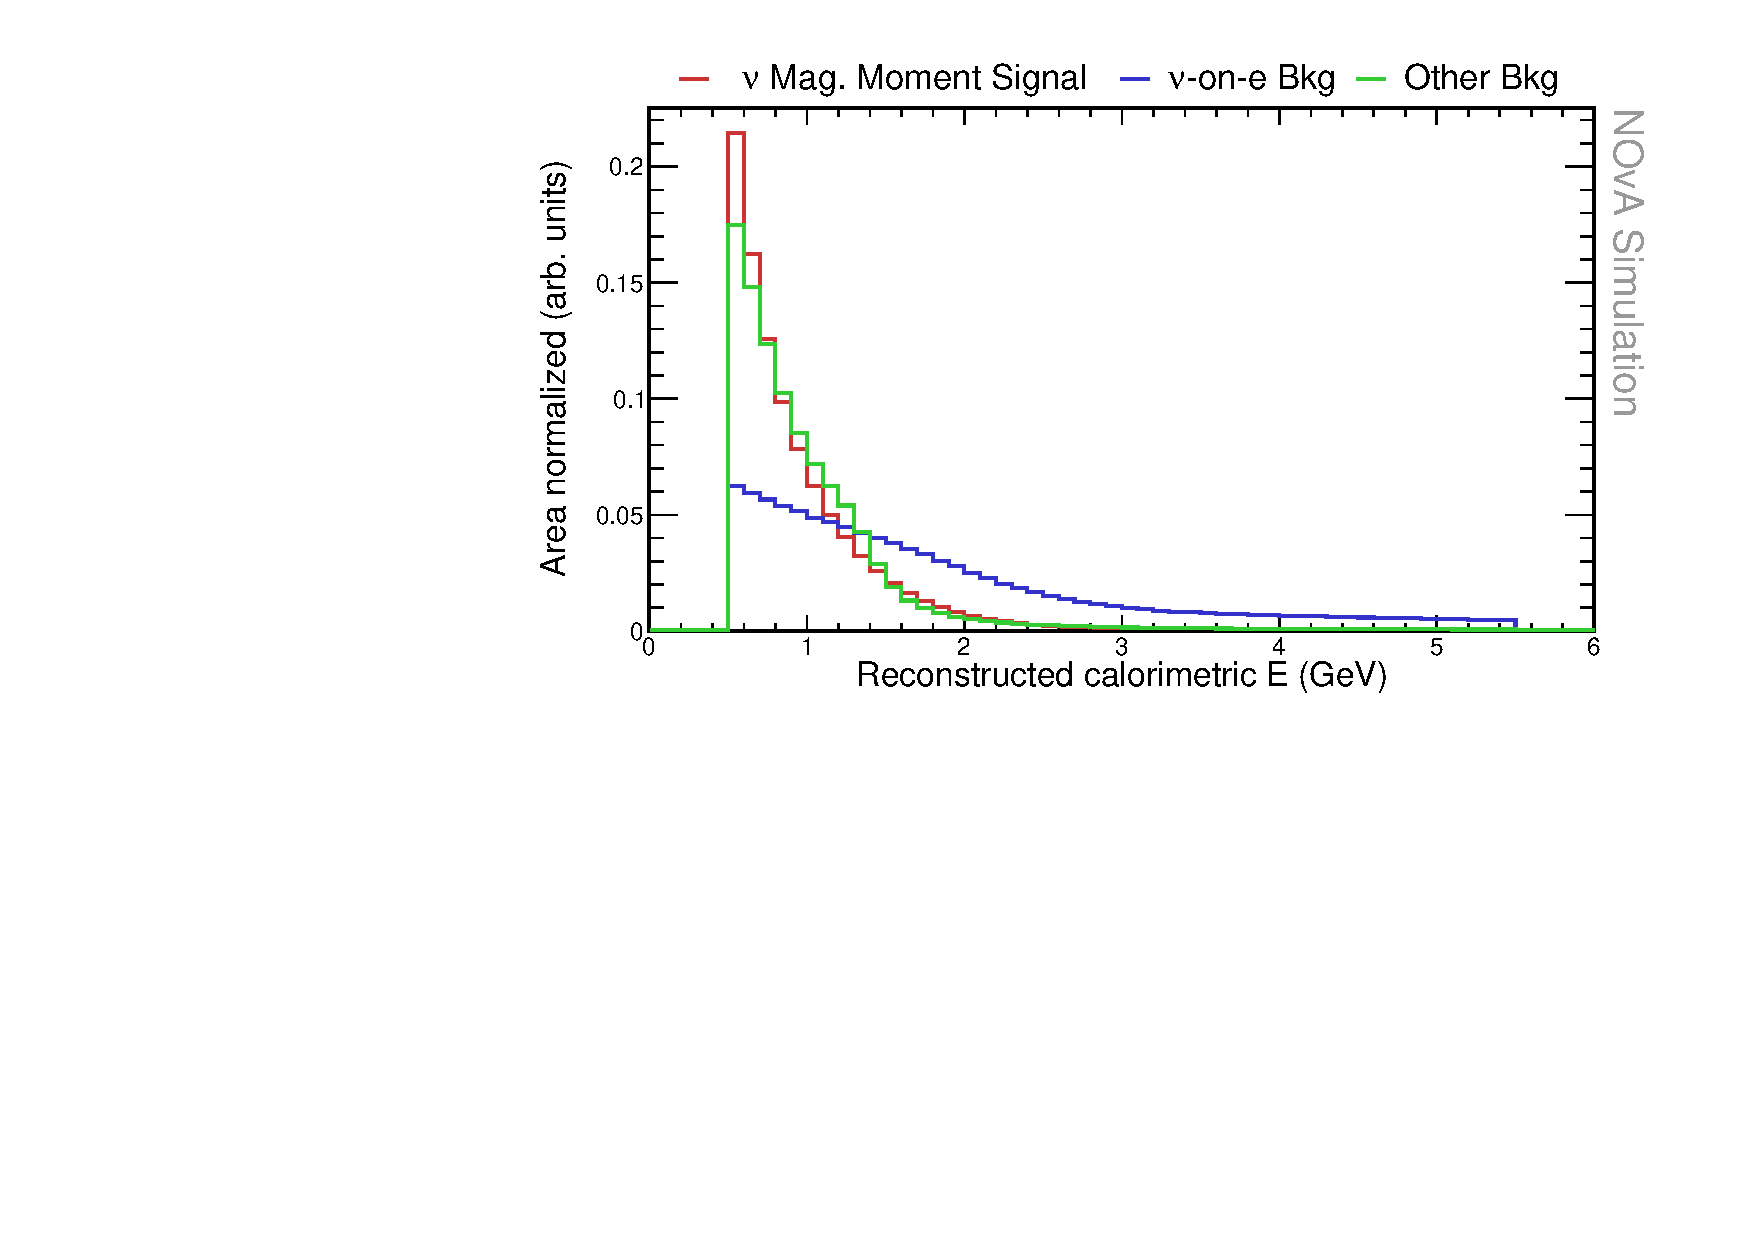
\includegraphics[width=.9\textwidth]{Plots/NuMMEventSelection/N1Cut_calEHighPre.pdf}
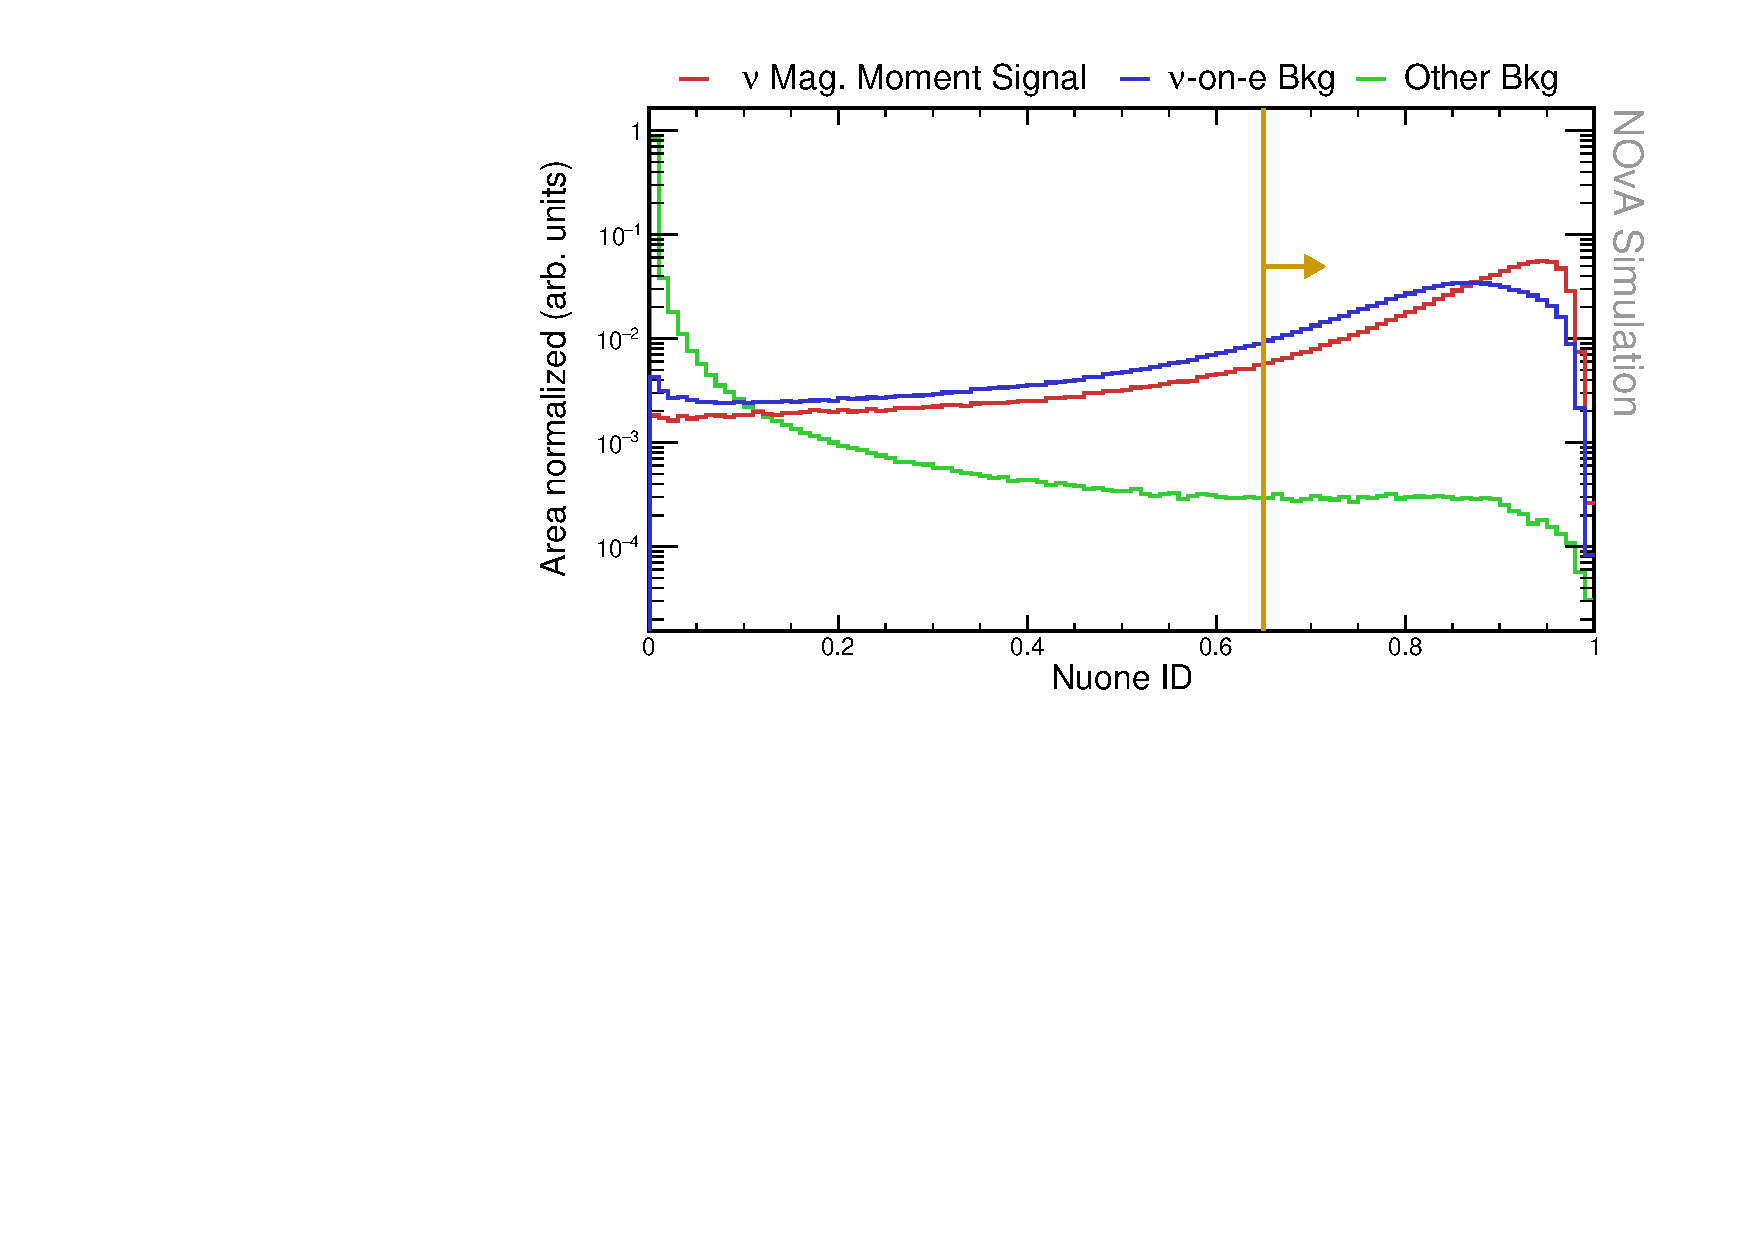
\includegraphics[width=.9\textwidth]{Plots/NuMMEventSelection/LogY_N1Cut_nuoneidPre.pdf}
\caption{Relative comparison of signal, $\nu$-on-e background, and other background events for the reconstructed vertex. No cuts were applied to make these plots. All the previous cuts were applied, including the cut on the shower energy. No single particle or event ID cuts were applied yet though. Gold lines show the cut values that create the fiducial volume.}
\label{fig:SingleShowerCuts}
\end{figure}

\begin{figure}[hbtp]
\centering
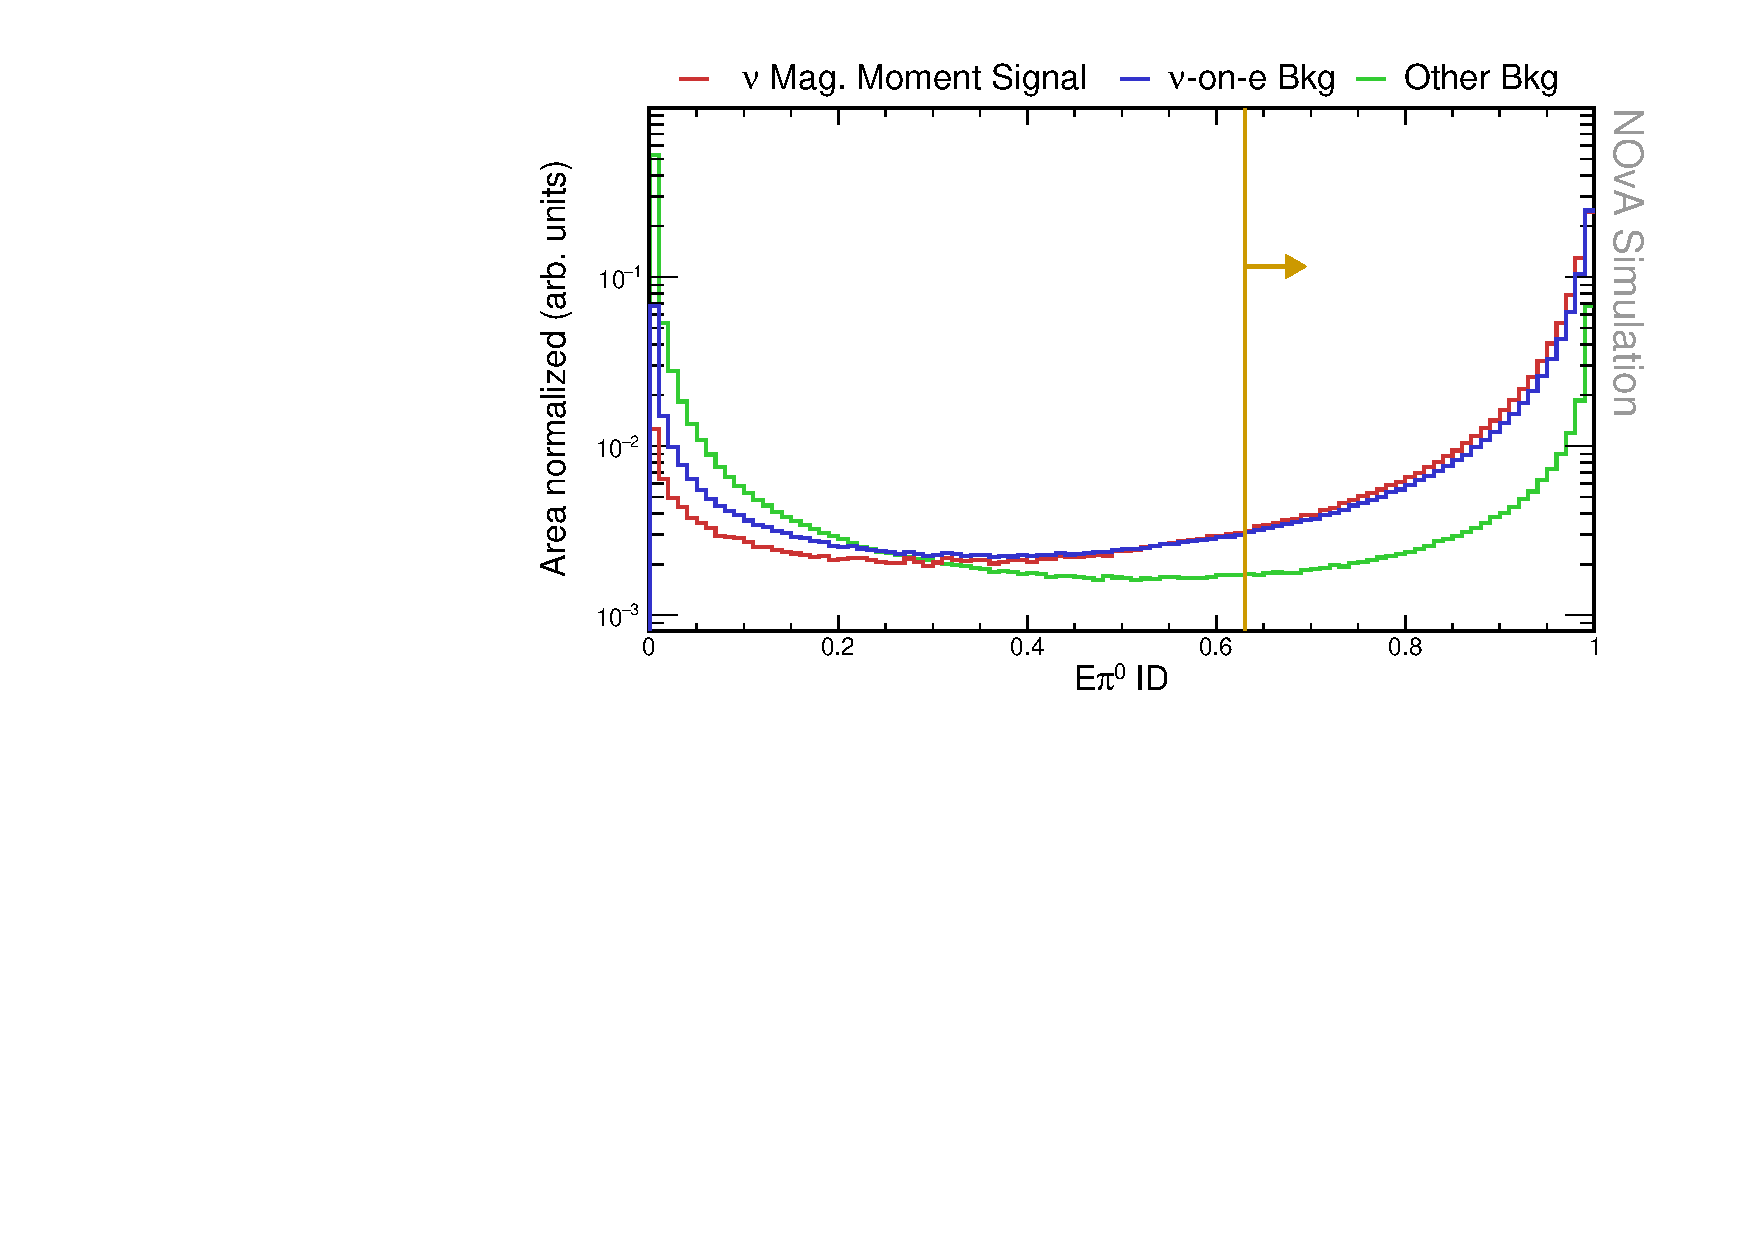
\includegraphics[width=.9\textwidth]{Plots/NuMMEventSelection/LogY_N1Cut_epi0idPre.pdf}
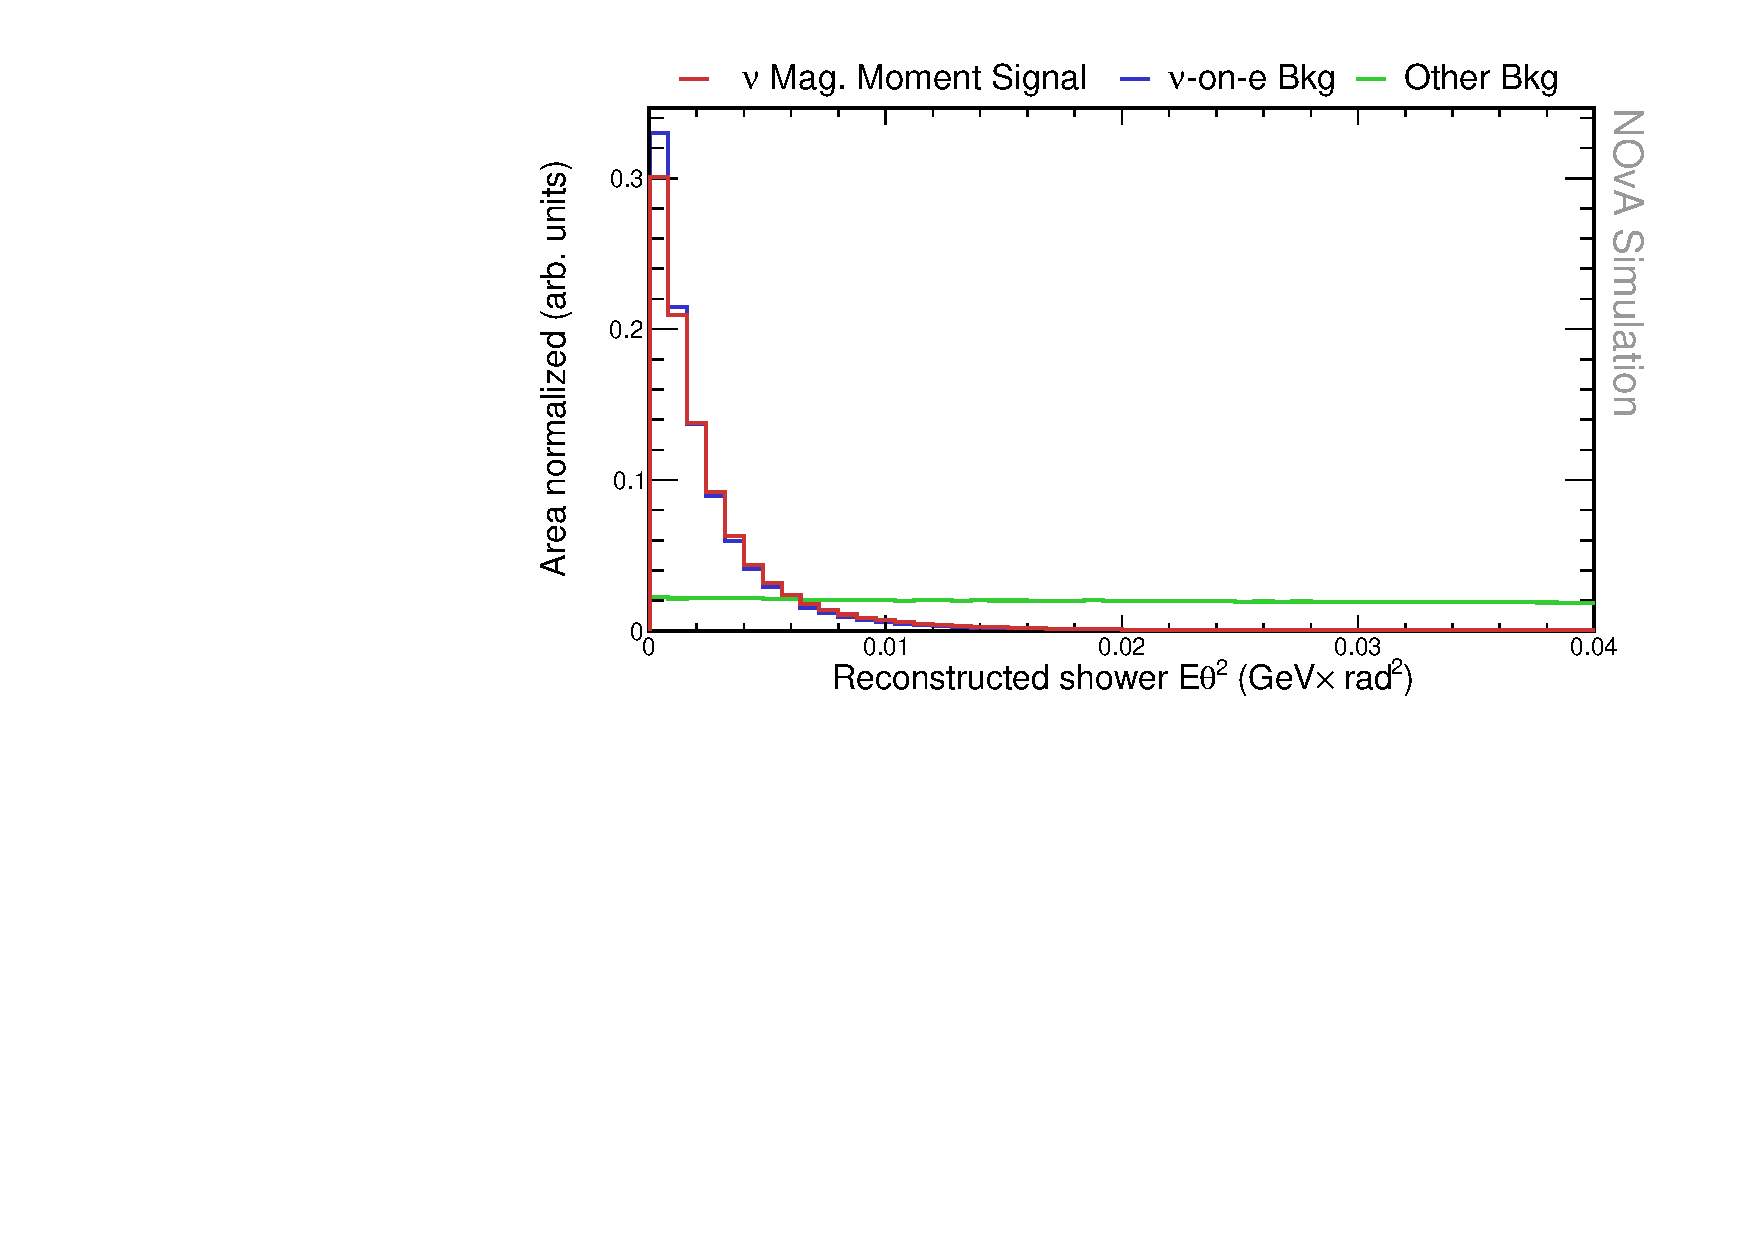
\includegraphics[width=.9\textwidth]{Plots/NuMMEventSelection/N1Cut_eth2Pre.pdf}
\caption{Relative comparison of signal, $\nu$-on-e background, and other background events for the reconstructed vertex. No cuts were applied to make these plots. All the previous cuts were applied, including the cut on the shower energy. No single particle or event ID cuts were applied yet though. Gold lines show the cut values that create the fiducial volume.}
\label{fig:SingleShowerCuts}
\end{figure}

\subsubsection*{Event Classifiers}

We are using two event classifiers based on convolution neural network that were developed specifically to identify $\nu$-on-e interactions. The first one (\texttt{NuoneID}) is trained to select $\nu$-on-e events and the second one (\texttt{Epi0ID}) is trained on the events passing the \texttt{NuoneID} to reject the $\pi^0$ background. Our selection requires that \texttt{NuoneID}$>0.73$ and that \texttt{Epi0ID}$>0.92$.

\todo{reference theory for the kinematics of nuone scattering}
We require that the product of reconstructed energy of the primary shower and the square of its angle from the Z axis is $E_{cal}\theta^2<0.005\ \unit{GeV\times rad^2}$.

\todo{Add plots of distributions of the event selection variables with two columns. LHS shows no cuts applied and RHS shows all previous cuts applied}

Using the many plots below that show the effect of each of the cuts on the signal and all background events. (For signal we are showing NuMM=...)

[ND group's technote] Two event classifiers (NuoneID and Epi0ID) based on convolutional neural network (CNN) are trained to identify nuone elastic scattering events (NuoneID) and to further reject background with pi0 in the final state (Epi0ID). The CNN architecture adopted for this analysis is the one used for NOvA CVN [12]. It takes the pixel map of a slice as the input and has deeper and more complicated neural networks than the ANNs used in the previous round of analysis [11]. The training for both classifiers (NuoneID and Epi0ID) were done with single electron samples as the signal in order to mitigate the model dependence. A nuone elastic scattering has an electron in the final state which could deposit energy in the detector. Single electron events share this feature with nuone elastic scattering, but have more uniform distribution of energy, angle between the shower direction and the beam direction. This additional feature could prevent CNN models from overfitting the feature of the very small scattering angle.  To make comparisons, test samples of signal and background are normalized to 1.1E21. The output categories are \gls{nuone}, $\pi^0$, $\nu_e$\gls{CC} and other. The \gls{nuone} and $\pi^0$ outputs are used for the training of the Epi0ID. The pre-selection applied is: ND group's preselection ($L<\unit[800]{cm}$, $N_{plane}<120$, $N_{cell}<600$), loose containment ($-190<X<190$, $-190<Y<190$, $50<Z<1500$ $\unit{cm}$), loose single particle cut ($E_{vtx}<\unit[0.05]{GeV}$, $gap<\unit[20]{cm}$, $E_{shower}/E_{tot} > 0.9$ \note{These are quite strict actually}. The training accuracy for NuoneID is about 85\% and for Epi0ID is about 96\%. After each round of training, the trained model is saved to make predictions on the test sample so we know how the actual performance of the classifiers evolves over different epochs.

\subsubsection*{Multivariate Analysis}
TMVA \cite{TMVA}

These event selection in total reduces signal $\unit[44.51]{\%}$, \gls{nuone} background $\unit[70.40]{\%}$ and other background $\unit[99.97]{\%}$. After the full event selection, the predicted number of signal events for $\mu_\nu=10^{-9}\mu_B$ is $23.31$ and the total number of background events under the \gls{SM} hypothesis is $678.26$. The most likely improvement is in probing the low energetic events and making sure they make sense. Additionally, it is possible to use a specially designed control regions to mitigate the very high non-\gls{nuone} background.

\begin{table}[!hb]
\centering
\caption[Event selection cutflow table]{Event selection cutflow table for the reconstruction quality cuts showing the number of events and the relative efficiency of each cut for each signal sample. The relative efficiency is calculated as number of events remaining after applying the corresponding cut divided by number of event for all the previous cuts. All the cuts are listed in sequence as they are applied.}
\begin{tabular}{|l|cc|cc|cc|}\hline
\multicolumn{1}{|c|}{} & \multicolumn{2}{c|}{\textbf{Signal}} & \multicolumn{2}{c|}{\textbf{$\nu$-on-e bkg}} & \multicolumn{2}{c|}{\textbf{Other bkg}} \\
\multicolumn{1}{|c|}{\multirow{-2}{*}{\textbf{Selection}}} & \textbf{$N_{evt}$} & \textbf{$\epsilon_{rel}\left(\%\right)$} & \textbf{$N_{evt}$} & \textbf{$\epsilon_{rel}\left(\%\right)$}  & \textbf{$N_{evt}$} & \textbf{$\epsilon_{rel}\left(\%\right)$}\\\hline
\textbf{Pre-selection} & 42.01 & 100 & 1.62$\times 10^3$ & 100 & 7.22$\times 10^5$ & 100\\
\textbf{$E_{Shower}/E_{Tot}$} & 40.32 & 95.98 & 1.57$\times 10^3$ & 96.87 & 2.79$\times 10^5$ & 38.60\\
\textbf{N$^o$ Hits} & 39.93 & 99.03 & 1.34$\times 10^3$ & 85.56 & 2.63$\times 10^5$ & 94.24\\
\textbf{High $E_{Shower}$} & 34.70 & 86.91 & 714.28 & 53.28 & 2.22$\times 10^5$ & 84.58\\
\textbf{\gls{nuone} ID} & 29.41 & 84.75 & 600.38 & 84.05 & 3.36$\times 10^3$ & 1.51\\
\textbf{$E\pi^0$ ID} & 27.46 & 93.37 & 560.56 & 93.37 & 2.18$\times 10^3$ & 64.72\\
\textbf{$E\theta^2$} & 23.31 & 84.88 & 478.83 & 85.42 & 199.42 & 9.17\\\hline
\end{tabular}
\label{tab:CutflowTableFiducialContainmnet}
\end{table}


\iffalse
\todo{Describe the cutflow tables below}
The final event count and efficiency of each of the cuts is shown on the table \ref{tab:CutflowTableSignal}. Table \ref{tab:CutflowTableBackground} shows the dissemination of background into the individual components.

\begin{table}[!hb]
\caption{Event selection cutflow table}
\begin{tabular}{|l|ccc|ccc|ccc|}\hline
\multicolumn{1}{|c|}{}                                     & \multicolumn{3}{c|}{\textbf{$\nu$ Mag. Moment signal}}          & \multicolumn{3}{c|}{\textbf{$\nu$-on-e background}}                      & \multicolumn{3}{c|}{\textbf{Other background}}                           \\
\multicolumn{1}{|c|}{\multirow{-2}{*}{\textbf{Selection}}} & \multicolumn{1}{c}{\textbf{$N_{sig}$}} & \textbf{$\epsilon^{N-1}$} & \textbf{$\epsilon \left(\%\right)$} & \multicolumn{1}{c}{\textbf{$N_{IBkg}$}} & \textbf{$\epsilon^{N-1}$} & \textbf{$\epsilon \left(\%\right)$} & \multicolumn{1}{c}{\textbf{$N_{Bkg}$}} & \textbf{$\epsilon^{N-1}$} & \textbf{$\epsilon \left(\%\right)$} \\\hline
\textbf{No Cut}      & 269.77            & 100 & 100 & 3.43$\times 10^3$           & 100 & 100                                     & 2.96$\times 10^8$          & 100                                                             & 100                                    \\
\textbf{Vtx Is Valid}  & 180.58            & 66.94                                                              & 66.94                                     & 3.33$\times 10^3$               & 96.94                                                               & 96.94                                      & 2.34$\times 10^8$          & 79.09                                                              & 79.09                                     \\
\textbf{N Prongs}        & 174.69            & 96.74                                                              & 64.76                                     & 3.23$\times 10^3$                             & 96.99                                                               & 94.02                                      & 8.66$\times 10^7$                     & 37.00                                                                 & 29.27                                     \\
\textbf{Png Length}  & 174.67            & 99.99                                                              & 64.75                                     & 3.22$\times 10^3$                                          & 99.64                                                               & 93.68                                      & 7.67$\times 10^7$                              & 88.56                                                              & 25.92                                     \\
\textbf{N Planes}      & 174.67            & 100                                                                & 64.75                                     & 3.22$\times 10^3$                                          & 99.98                                                               & 93.67                                      & 7.67$\times 10^7$          & 99.98                                                              & 25.92                                     \\
\textbf{N Cells}       & 174.67            & 100                                                                & 64.75                                     & 3.22$\times 10^3$                                           & 99.98                                                               & 93.65                                      & 7.42$\times 10^7$          & 96.78                                                              & 25.08                                     \\
\textbf{Closest Slc}  & 169.82            & 97.22                                                              & 62.95                                     & 3.14$\times 10^3$                                           & 97.54                                                               & 91.35                                      & 6.95$\times 10^7$          & 93.68                                                              & 23.49 \\
\textbf{Fiducial}     & 167.72            & 98.76                                                              & 62.17                                     & 3.09$\times 10^3$           & 98.41                                                               & 89.89                                      & 3.59$\times 10^7$          & 51.71                                                              & 12.15                                     \\
\textbf{Cont.}  & 159.37            & 95.02                                                              & 59.08                                     & 2.48$\times 10^3$           & 80.43                                                               & 72.30                                      & 1.38$\times 10^7$          & 38.35                                                              & 4.66                                      \\
\textbf{ShwE Frac.}  & 150.37            & 94.35                                                              & 55.74                                     & 2.42$\times 10^3$           & 97.59                                                               & 70.56                                      & 8.82$\times 10^6$          & 63.97                                                              & 2.98                                      \\
\textbf{Vtx E}         & 142.29            & 94.63                                                              & 52.74                                     & 2.18$\times 10^3$           & 90.16                                                               & 63.62                                      & 4.15$\times 10^6$          & 47.07                                                              & 1.40                                      \\
\textbf{Shw Gap}          & 137.96            & 96.96                                                              & 51.14                                     & 2.09$\times 10^3$           & 95.58                                                               & 60.80                                      & 3.25$\times 10^6$          & 78.34                                                              & 1.10                                      \\
\textbf{Shw E}      & 37.13             & 26.92                                                              & 13.76                                     & 1.36$\times 10^3$           & 65.10                                                               & 39.58                                      & 6.25$\times 10^5$          & 19.21                                                              & 0.21                                      \\
\textbf{Nuoneid}      & 29.48             & 79.39                                                              & 10.93                                     & 940.21             & 69.18                                                               & 27.38                                      & 2.42$\times 10^4$ & 3.88                                                               & 8.19$\times 10^{-3}$                                  \\
\textbf{Epi0id}       & 22.51             & 76.35                                                              & 8.34                                      & 749.93             & 79.76                                                               & 21.84                                      & 1.47$\times 10^4$ & 60.75                                                              & 4.97$\times 10^{-3}$                                  \\
\rowcolor[HTML]{67FD9A}
\textbf{$E\theta^2$}      & 19.74             & 87.73                                                              & 7.32                                      & 675.02             & 90.01                                                               & 19.66                                      & 84.15             & 0.57                                                               & 2.84$\times 10^{-5}$                                 \\\hline\hline
\textbf{$E\theta^2$ (sb)}  & 2.74              & -                                                              & 1.01                                      & 74.30              & -                                                               & 2.16                                       & 1.01$\times 10^3$          & - & 3.43$\times 10^{-4}$                                  \\\hline\hline
\textbf{No ShwE}  & 37.62             & -                                                           & 13.94                                     & 782.67             & -                                                            & 22.79                                      & 238.79            & -                                                              & 8.07E-05   \\\hline
\end{tabular}
\label{tab:CutflowTableSignal}
\end{table}

%\begin{landscape}
\begin{sidewaysfigure}[!hb]
\caption{Event selection cutflow table for background components}
\begin{scriptsize}
%\begin{table}[!hb]
\begin{tabular}{|l|ccc|ccc|ccc|ccc|ccc|}\hline
\multicolumn{1}{|c|}{\multirow{2}{*}{\textbf{Selection}}} & \multicolumn{3}{c|}{\textbf{$\nu_e$CC MEC}} &
\multicolumn{3}{c|}{\textbf{$\nu_e$CC Other}} &
\multicolumn{3}{c|}{\textbf{$\nu_\mu$CC}} &
\multicolumn{3}{c|}{\textbf{NC}} &
\multicolumn{3}{c|}{\textbf{Other}} \\
\multicolumn{1}{|c|}{}                                    & \multicolumn{1}{c}{\textbf{$N$}} & \textbf{$\epsilon^{N-1}$} & \textbf{$\epsilon \left(\%\right)$} & \multicolumn{1}{c}{\textbf{$N$}} & \textbf{$\epsilon^{N-1}$} & \textbf{$\epsilon \left(\%\right)$} & \multicolumn{1}{c}{\textbf{$N$}} & \textbf{$\epsilon^{N-1}$} & \textbf{$\epsilon \left(\%\right)$} & \multicolumn{1}{c}{\textbf{$N$}} & \textbf{$\epsilon^{N-1}$} & \textbf{$\epsilon \left(\%\right)$} & \multicolumn{1}{c}{\textbf{$N$}} & \textbf{$\epsilon^{N-1}$} & \textbf{$\epsilon \left(\%\right)$} \\\hline
\textbf{No Cut}      & 3.50$\times 10^4$           & 100 & 100                                     & 3.23$\times 10^6$             & 100 & 100 & 2.24$\times 10^8$              & 100                                                                 & 100                                        & 3.40$\times 10^7$          & 100.                                                             & 100                                    & 3.49$\times 10^7$                      & 100 & 100                                       \\
\textbf{Vtx Is Valid}  & 3.27$\times 10^4$           & 93.58                                                               & 93.58                                      & 2.62$\times 10^6$             & 81.14                                                                 & 81.14                                        & 1.99$\times 10^8$              & 89.02                                                                  & 89.02                                         & 2.57$\times 10^7$ & 75.55                                                              & 75.55                                     & 6.53$\times 10^6$             & 18.70                                                                 & 18.70                                        \\
\textbf{N Prongs}        & 2.74$\times 10^4$           & 83.76                                                               & 78.39                                      & 1.39$\times 10^6$             & 53.05                                                                 & 43.05                                        & 6.75$\times 10^7$              & 33.89                                                                  & 30.17                                         & 1.51$\times 10^7$          & 58.57                                                              & 44.25                                     & 2.65$\times 10^6$ & 40.51                                                                 & 7.58                                         \\
\textbf{Png Length}  & 2.73$\times 10^4$           & 99.79                                                               & 78.22                                      & 1.37$\times 10^6$             & 98.53                                                                 & 42.42                                        & 5.77$\times 10^7$ & 85.56                                                                  & 25.81                                         & 1.49$\times 10^7$          & 99.07                                                              & 43.84                                     & 2.64$\times 10^6$             & 99.87                                                                 & 7.57                                         \\
\textbf{N Planes}      & 2.73$\times 10^4$           & 99.99                                                               & 78.22                                      & 1.37$\times 10^6$             & 99.99                                                                 & 42.41                                        & 5.77$\times 10^7$              & 99.98                                                                  & 25.81                                         & 1.49$\times 10^7$          & 100                                                             & 43.84                                     & 2.64$\times 10^6$ & 100                                                                & 7.57                                         \\
\textbf{N Cells}       & 2.73$\times 10^4$           & 99.99                                                               & 78.21                                      & 1.28$\times 10^6$             & 93.49                                                                 & 39.65                                        & 5.59$\times 10^7$ & 96.82                                                                  & 24.98                                         & 1.44$\times 10^7$          & 96.34                                                              & 42.24                                     & 2.64$\times 10^6$             & 100                                                                & 7.57                                         \\
\textbf{Closest Slc}  & 2.73$\times 10^4$           & 99.79                                                               & 78.05                                      & 1.21$\times 10^6$ & 94.25                                                                 & 37.37                                        & 5.33$\times 10^7$ & 95.40                                                                  & 23.84                                         & 1.35$\times 10^7$          & 94.17                                                              & 39.77                                     & 1.43$\times 10^6$ & 54.22                                                                 & 4.10 \\
\textbf{Fiducial}     & 1.39$\times 10^4$           & 51.12                                                               & 39.90                                      & 6.30$\times 10^5$ & 52.10                                                                 & 19.47                                        & 2.60$\times 10^7$          & 48.77                                                                  & 11.62                                         & 8.25$\times 10^6$          & 60.99                                                              & 24.26                                     & 1.05$\times 10^6$             & 73.53                                                                 & 3.02                                         \\
\textbf{Cont.}  & 9.32$\times 10^3$           & 66.82                                                               & 26.66                                      & 2.63$\times 10^5$             & 41.72                                                                 & 8.12                                         & 7.64$\times 10^6$              & 29.38                                                                  & 3.42                                          & 4.96$\times 10^6$          & 60.15                                                              & 14.59                                     & 9.12$\times 10^5$             & 86.62                                                                 & 2.61                                         \\
\textbf{ShwE Frac.}  & 9.20$\times 10^3$           & 98.70                                                               & 26.32                                      & 1.95$\times 10^5$             & 74.39                                                                 & 6.04                                         & 4.82$\times 10^6$              & 63.10                                                                  & 2.15                                          & 2.97$\times 10^6$          & 59.78                                                              & 8.72                                      & 8.28$\times 10^5$             & 90.81                                                                 & 2.37                                         \\
\textbf{Vtx E}         & 5.92$\times 10^3$           & 64.33                                                               & 16.93                                      & 6.05$\times 10^4$             & 30.96                                                                 & 1.87                                         & 1.97$\times 10^6$ & 40.79                                                                  & 0.88                                          & 1.36$\times 10^6$          & 45.75                                                              & 3.99                                      & 7.62$\times 10^5$             & 92.03                                                                 & 2.18                                         \\
\textbf{Shw Gap}          & 5.50$\times 10^3$           & 92.91                                                               & 15.73                                      & 4.62$\times 10^4$             & 76.40                                                                 & 1.43                                         & 1.58$\times 10^6$ & 80.18                                                                  & 0.70                                          & 1.06$\times 10^6$          & 77.78                                                              & 3.10                                      & 5.69$\times 10^5$             & 74.61                                                                 & 1.63                                         \\
\textbf{Shw E}      & 3.62$\times 10^3$           & 65.81                                                               & 10.35                                      & 1.12$\times 10^4$             & 24.15                                                                 & 0.35                                         & 4.38$\times 10^5$              & 27.80                                                                  & 0.20                                          & 1.71$\times 10^5$          & 16.15                                                              & 0.50                                      & 1.28$\times 10^3$             & 0.23                                                                  & 3.68$\times 10^{-3}$                                     \\
\textbf{Nuoneid}      & 1.40$\times 10^3$           & 38.63                                                               & 4.00                                       & 2.11$\times 10^3$             & 18.89                                                                 & 0.065                                        & 1.17$\times 10^4$              & 2.66                                                                   & 5.21$\times 10^{-3}$                                      & 8.99$\times 10^3$          & 5.27                                                               & 0.026                                     & 66.43                & 5.17                                                                  & 1.90$\times 10^{-4}$                                     \\
\textbf{Epi0id}       & 1.14$\times 10^3$           & 81.78                                                               & 3.27                                       & 1.61$\times 10^3$             & 76.40                                                                 & 0.050                                        & 7.17$\times 10^3$              & 61.52                                                                  & 3.20$\times 10^{-3}$                                      & 4.76$\times 10^3$          & 52.94                                                              & 0.014                                     & 29.47                & 44.36                                                                 & 8.44$\times 10^{-5}$                                     \\
\rowcolor[HTML]{67FD9A}
\textbf{$E\theta^2$}      & 15.13              & 1.32                                                                & 0.043                                      & 39.00                & 2.42                                                                  & 1.21$\times 10^{-3}$                                     & 8.62                  & 0.12                                                                   & 3.85$\times 10^{-6}$                                      & 20.91             & 0.44                                                               & 6.15$\times 10^{-5}$                                  & 0.50                 & 1.69                                                                  & 1.43$\times 10^{-6}$                                  \\\hline\hline
\textbf{$E\theta^2$ (sb)}  & 386.16             & -                                                            & 1.10                                       & 306.55               & -                                                                & 9.48$\times 10^{-3}$                                     & 165.59                & -                                                               & 7.40$\times 10^{-5}$                                      & 149.93            & -                                                             & 4.41$\times 10^{-4}$                                  & 6.24                 & -                                                              & 1.79$\times 10^{-5}$                                     \\\hline\hline
\textbf{No ShwE}  & 15.54              & -                                                                & 0.044                                      & 69.61                & -                                                                 & 2.15$\times 10^{-3}$                                     & 68.48                 & - & 3.06$\times 10^{-5}$                                      & 75.67             & - & 2.22$\times 10^{-4}$                                  & 9.49                 & -                                                                & 2.72E-05   \\\hline
\end{tabular}

\label{tab:CutflowTableBackground}
%\end{table}
\end{scriptsize}
\end{sidewaysfigure}
%\end{landscape}
\fi

\todo{Add a discussion of possible improvements on the event selection on its limitations - mostly for the analysis review committee}
From here we can see that ... Maybe what can be improved is...
This can likely be improved upon by specifically selection low energy events and removing the cut on the reconstructed shower energy. 


%%%%%%%%%%%%%%%%%%%%%%%%%%%%%%%%%%%%%%%%%%%%%%%%%%%%%%%%%%%%%%%%%%%%%
%%%                   RESOLUTION AND BINNING                      %%%
%%%%%%%%%%%%%%%%%%%%%%%%%%%%%%%%%%%%%%%%%%%%%%%%%%%%%%%%%%%%%%%%%%%%%
\section{Energy resolution and binning}\label{sec:NuMMResolution}
\todo{Add the energy resolution and binning plots}
Describe what events were used for the energy resolution study and how it was performed

What are the results

Final plot

The electron energy and angle distributions and resolutions. Are we going to fit in E, Th, or ETh2? Is there something else?

Show plots of Reco V True for both energy and angle. (Should I show it with or without the energy cut?). Also show the resolution plots.

Maybe also mention that Test Beam will help with improving the dead materials correction and generally improving the bias and resolution of the reconstructed energy, which won't have to depend on the comparison to simulation

%%%%%%%%%%%%%%%%%%%%%%%%%%%%%%%%%%%%%%%%%%%%%%%%%%%%%%%%%%%%%%%%%%%%%
%%%                    SYSTEMATIC UNCERTAINTIES                   %%%
%%%%%%%%%%%%%%%%%%%%%%%%%%%%%%%%%%%%%%%%%%%%%%%%%%%%%%%%%%%%%%%%%%%%%
\section{Systematic uncertainties}\label{sec:NuMMSystematics}
\iffalse
\todo{Describe the main systematic uncertainties. Add plots showing their effect on the NuMM events. Possibly with different event selection variables as X axes. Also show the final table with the percentages summed}
Plots showing combined uncertainties for signal and backgrounds. Maybe also some interpolations. Table of systematic uncertainties on the event count.

Ideally should also talk about what measures were used to mitigate the systematic uncertainties, but there were none...

\subsubsection*{Normalization systematics}
\todo{Describe the normalization systematics (or just remove this if not using them in the end}
Should we include normalization systematics? Would that make any difference? There's a POT scaling uncertainty which is very small (find out exactly how small).

In the fitting experiment normalization uncertainties would probably not make any difference whatsoever, but in the counting experiment they might be important?

\subsubsection*{Neutrino flux systematics}
\todo{Describe the flux uncertainties. Describe the PCA. Describe the difference between what the ND group is doing and what we're doing}
Using the PCA vs using the PPFX universes+beam transport separately. Plots of energy showing shifts for signal and backgrounds separately

\todo{understand differences with ND and 3F methods}

This is mainly a normalization. Discuss how to use the fact that $\nu$-on-e events can be used (and are used) to constraint the beam uncertainty. Would the counting experiment still be valid then? Maybe if we made another sideband sample...

\subsubsection*{Detector systematics}
\todo{Make plots of energy showing shifts for signal and backgrounds separately}
Reference for the Prod5.1 detector systematics is docdb 53225

\subsubsection*{Cross section systematics}
\todo{Describe the XSec systs}
Only for the non nu-on-e background. Assuming the nu-on-e events (including the signal events) are precisely known.

Plots of energy showing shifts for signal and backgrounds separately
\fi


%%%%%%%%%%%%%%%%%%%%%%%%%%%%%%%%%%%%%%%%%%%%%%%%%%%%%%%%%%%%%%%%%%%%%
%%%                           FITTING                             %%%
%%%%%%%%%%%%%%%%%%%%%%%%%%%%%%%%%%%%%%%%%%%%%%%%%%%%%%%%%%%%%%%%%%%%%
\section{Statistical analysis}\label{sec:NuMMFitting}

We are basically doing two separate things:
\begin{enumerate}
\item Testing a hypothesis that there is no magnetic moment present in the signal. Can we reject the null hypothesis given our data?
\item If we can reject the null hypothesis we want to estimate the best fit of the parameter. Additionally, we want to put a limit (set a confidence interval) on the magnetic moment parameter.
\end{enumerate}

What should be included here:
\begin{itemize}
\item Fit methodology: Detail the fitting techniques used to extract the muon neutrino magnetic moment from the data.
\item Fit validation: Describe how the fit is validated, including any statistical tests used.
\item Fake data studies: Explain the use of fake data or Monte Carlo simulations to test the robustness of the analysis.
\end{itemize}

\iffalse
Depends on what fits I'm going to end up using...

How do we find the value of or limit for the effective neutrino magnetic moment?

Large section on statistics in the PDG.

Maximum likelihood with binned data:

N bins with a vector of data $n=\left(n1,...,n_N \right)$ with expectation values $\mu=E\left[n\right]$ and probabilities $f\left(n;\mu\right)$. Suppose the mean values $\mu$ can be determined as a function of a set of parameters $\theta$ (I assume for us there's either only one parameter - magnetic moment, or three parameters - mag. moment, scale of SM signal and scale of SM background). Then one may maximize the likelihood function based on the contents of the bins.

If the $n_i$ is regarded as independent and Poisson distributed (which I'd say is the case for us), then the data are instead described by a product of Poisson probabilities,
\begin{equation}
f_p\left(n;\theta\right)=\prod_{i=1}^{N} \frac{\mu_i^{n_i}}{n_i!}e^{-\mu_i},
\end{equation}
where the mean values $\mu_i$ are given functions of $\theta$. The total number of events $n_{tot}$ thus follows a Poisson distribution with mean $\mu_{tot}=\sum_i \mu_i$.

When using maximum likelihood with binned data, one can find the maximum likelihood estimators and at the same time obtain a statistic usable for a test of goodness-of-fit. Maximizing the likelihood $L\left(\theta\right)=f_P\left(n;\theta\right)$ is equivalent to maximizing the likelihood ratio $\lambda\left(\theta\right)=f_P\left(n;\theta\right) / f\left(n;\hat{\mu}\right)$, where in the denominator $f\left(n;\hat{\mu}\right)$ is a model with an adjustable parameter for each bin, $\mu=\left(\mu_1,...,\mu_N\right)$, and the corresponding estimators are $\hat{\mu}=\left(n_1,...,n_N\right)$ (called the `saturated model').

Equivalently one often minimizes the quantity $-2\ln\lambda\left(\theta\right)$. For independent Poisson distributed $n_i$ this is
\begin{equation}
-2\ln\lambda\left(\theta\right)=2\sum_{i=1}^{N}\left[\mu_i\left(\theta\right)-n_i+n_i\ln\frac{n_i}{\mu_i\left(\theta\right)}\right],
\end{equation}
where for bins with $n_i=0$, the last term is zero. In our term $\mu_i\left(\theta\right)$ is the \textbf{expected number of events in bin i if magnetic moment is $\theta$} and $n_i$ is the observed (measured) number of events in that bin.

A smaller value of $-2\ln\lambda\left(\hat{\theta}\right)$ corresponds to better agreement between the data and the hypothesized form of $\mu\left(\theta\right)$. The value of $-2\ln\lambda\left(\hat{\theta}\right)$ can thus be translated into a \textbf{p-value as a measure of goodness-of-fit}. Assuming the model is correct, then according to \textbf{Wilk's theorem}, for \textbf{sufficiently large} $\mu_i$ and provided certain regularity conditions are met, \textbf{the minimum of $-2\ln\lambda$ follows a $\chi^2$ distribution.} If there are N bins and M fitter parameters, then the number of degrees of freedom for the $\chi^2$ distribution is $N-M$ if the data are threated as Poisson distributed - which they are for us.

The method of least squares coincides with the method of maximum likelihood in a special case where the independent variables are Gaussian distributed - so I suppose this means that if I have enough events in each single bin, then I could equate the method of log likelihood and the method of least squares...

\subsection{Nuisance parameters}
In general the model is not perfect, which is to say it cannot provide an accurate description of the data even at the most optimal point of its parameter space. As a result, the estimated parameters can have a systematic bias. One can improve the model by including in it additional parameters. That is, $P\left(x|\theta\right)$ is replaced by a more general model $P\left(x|\theta,\nu\right)$, which depends on parameters of interest $\theta$ and \textit{nuisance parameters} $\nu$. The additional parameters are not of intrinsic interest but must be included for the model to be sufficiently accurate for some point in the enlarged parameter space.

Although including additional parameters may eliminate or at least reduce the effect of systematic uncertainties, their presence will result in increased statistical uncertainties for the parameters of interest. This occurs because the estimators for the nuisance parameters and those of interest will in general be correlated, which results in an enlargement of the contour.

To reduce the impact of the nuisance parameters one often tries to constrain their values by means of control or calibration measurements, say, having data \textbf{y} (I assume for us this would represent a control sample - like they use in the ND group). For example, some components of y could represent estimates of the nuisance parameters, often from separate experiments. Suppose the measurements y are statistically independent from x and are described by a model $P\left(y|\nu\right)$. The joint model for both x and y is in this case therefore the product of the probabilities for x
and y, and thus the likelihood function for the full set of parameters is
\begin{equation}
L\left(\theta,\nu\right)=P\left(x|\theta,\nu\right)P\left(y|\nu\right).
\end{equation}
Note that in this case if one wants to simulate the experiment by means of Monte Carlo, both the primary and control measurements, x and y, must be generated for each repetition under assumption of fixed values for the parameters $\theta$ and $\nu$.

Using all of the parameters $\left(\theta,\nu\right)$  to find the statistical errors in the parameters of interest $\theta$ is equivalent to using the \textit{profile likelihood}, which depends only on $\theta$. It is defined as
\begin{equation}
L_p\left(\theta\right)=L\left(\theta,\hat{\nu}\left(\theta\right)\right),
\end{equation}
This equation is supposed to have double hat for the neutrino on RHS but that throws an error when compiling...
%L\left(\theta,\hat{\hat{\nu}}\left(\theta\right)\right),
where the double-hat notation indicates the profiled values of the parameters $\nu$, defined as values that maximize $L$ for the specified $\theta$.

\subsection{Unbinned parameter estimation}
If the total number of data values is small, the unbinned maximum likelihood method is preferred, since binning can only result in a loss of information, and hence the larger statistical errors for the parameter estimates.
Does't this mean that if the number of events for the neutrino magnetic moment analysis is small, it would be better to do a completely unbinned maximum likelihood method, instead of a single bin method?

\subsection{Template fit}
\todo{Describe the fitting framework, ideally with an example plot, maybe with some arrows}
How does the fitting framework work? It's based on the framework developed by Mu Wei for the Light Dark Matter analysis (ref.) which was developed together (is this fair?). Basic description of the framework.

Also this framework is used for both LDM and NuMM together. It is trivial to simply switch between including the NuMM or LDM in it. This was done to save space in creating predictions since our backgrounds are exactly the same (or at least they should be...). Theoretically this could be separated into two difference frameworks.

\begin{itemize}
\item <NDPredictionSingleElectron> Prediction class which holds the LDM as a special 2-D spectrum (not used for NuMM), and NuMM, $\nu$-on-e background, $\nu_e$CC MEC background and other background as simple 1-D spectra. Also scaling each spectra by...
\item <NDPredictionSystSingleElectron> class derived from PredictionInterp that takes in the NDPredictionSingleElectron and applies systematic shifts to it. Includes the interpolation/extrapolation between the systematic shifts.
\item FitVariables and what do they do
\item Fitter which does exactly what... What are the parameters of the fit? What are the results/outputs?
\end{itemize}
\fi

%%%%%%%%%%%%%%%%%%%%%%%%%%%%%%%%%%%%%%%%%%%%%%%%%%%%%%%%%%%%%%%%%%%%%
%%%                             RESULTS                           %%%
%%%%%%%%%%%%%%%%%%%%%%%%%%%%%%%%%%%%%%%%%%%%%%%%%%%%%%%%%%%%%%%%%%%%%
\section{Results}\label{sec:NuMMResults}

Show the money plot - full prediction in the binned energy distribution, including the full statistical and systematic uncertainties

Write out the total number of measured events and their corresponding uncertainties

Explain what are the results of the fit and the limits, discuss the statistical significance of the result

%%%%%%%%%%%%%%%%%%%%%%%%%%%%%%%%%%%%%%%%%%%%%%%%%%%%%%%%%%%%%%%%%%%%%
%%%                            DISCUSSION                         %%%
%%%%%%%%%%%%%%%%%%%%%%%%%%%%%%%%%%%%%%%%%%%%%%%%%%%%%%%%%%%%%%%%%%%%%
\section{Discussion}\label{sec:NuMMDiscussion}

What should be included here:
\begin{itemize}
\item Interpretation: Interpret the results in the context of the current understanding of neutrino physics.
\item Implications: Explain the broader implications of your findings for the field of particle physics.
\item Future work: Suggest directions for future research based on your results.
\begin{itemize}
\item Improvements in NOvA, more FHC data, including RHC data, better reconstruction, better simulation and calibration, better event selection, including sideband samples, more systematics studies, better fitting techniques...
\item Future beyond NOvA - DUNE
\begin{itemize}
\item What are the possibilities for DUNE?
\end{itemize}
\end{itemize}
\end{itemize}

%For the energy deposition of electron in LArTPC might be a good source this https://iopscience.iop.org/article/10.1088/1748-0221/15/03/P03022/pdf


%%%%%%%%%%%%%%%%%%%%%%%%%%%%%%%%%%%%%%%%%%%%%%%%%%%%%%%%%%%%%%%%%%%%%
%%%                            CONCLUSION                         %%%
%%%%%%%%%%%%%%%%%%%%%%%%%%%%%%%%%%%%%%%%%%%%%%%%%%%%%%%%%%%%%%%%%%%%%
\section{Conclusion}\label{sec:NuMMConclusion}

Summarize the results and compare them to the introduction, including comparisons to other experiments and theory. Restate the significant of the measurement

Closing remarks